\chapter[Backgrounds to $\Htautau$][Backgrounds to $\Htautau$]{Backgrounds to $\Htautau$}
\label{chap:backgrounds}

\begin{quote}
Background estimates in the $\Htautau$ analysis are described.
\end{quote}

\section{$\Ztautau$}
\label{sec:backgrounds-ztautau}

\begin{figure}[tp]
  \centering
  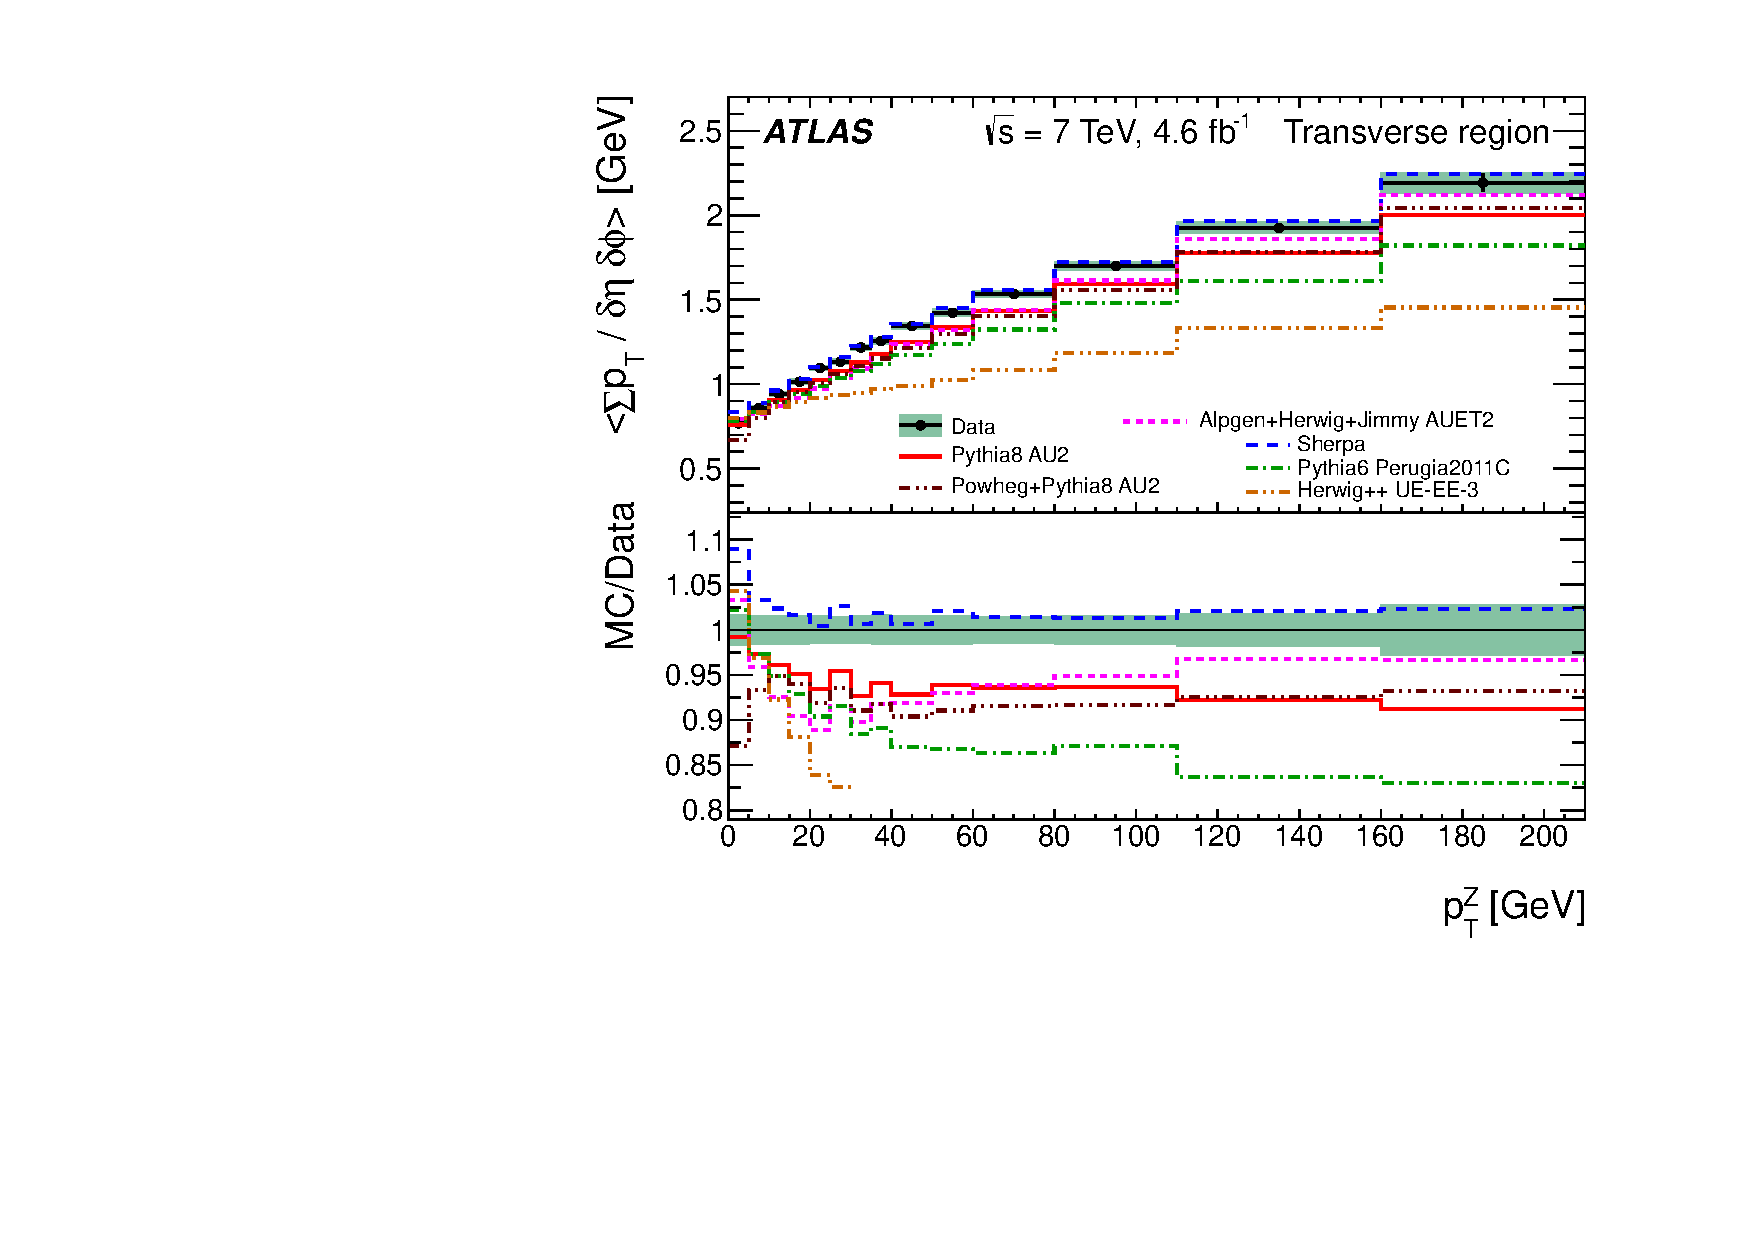
\includegraphics[width=0.48\textwidth]{figures/STDM-2011-42/fig_14b}
  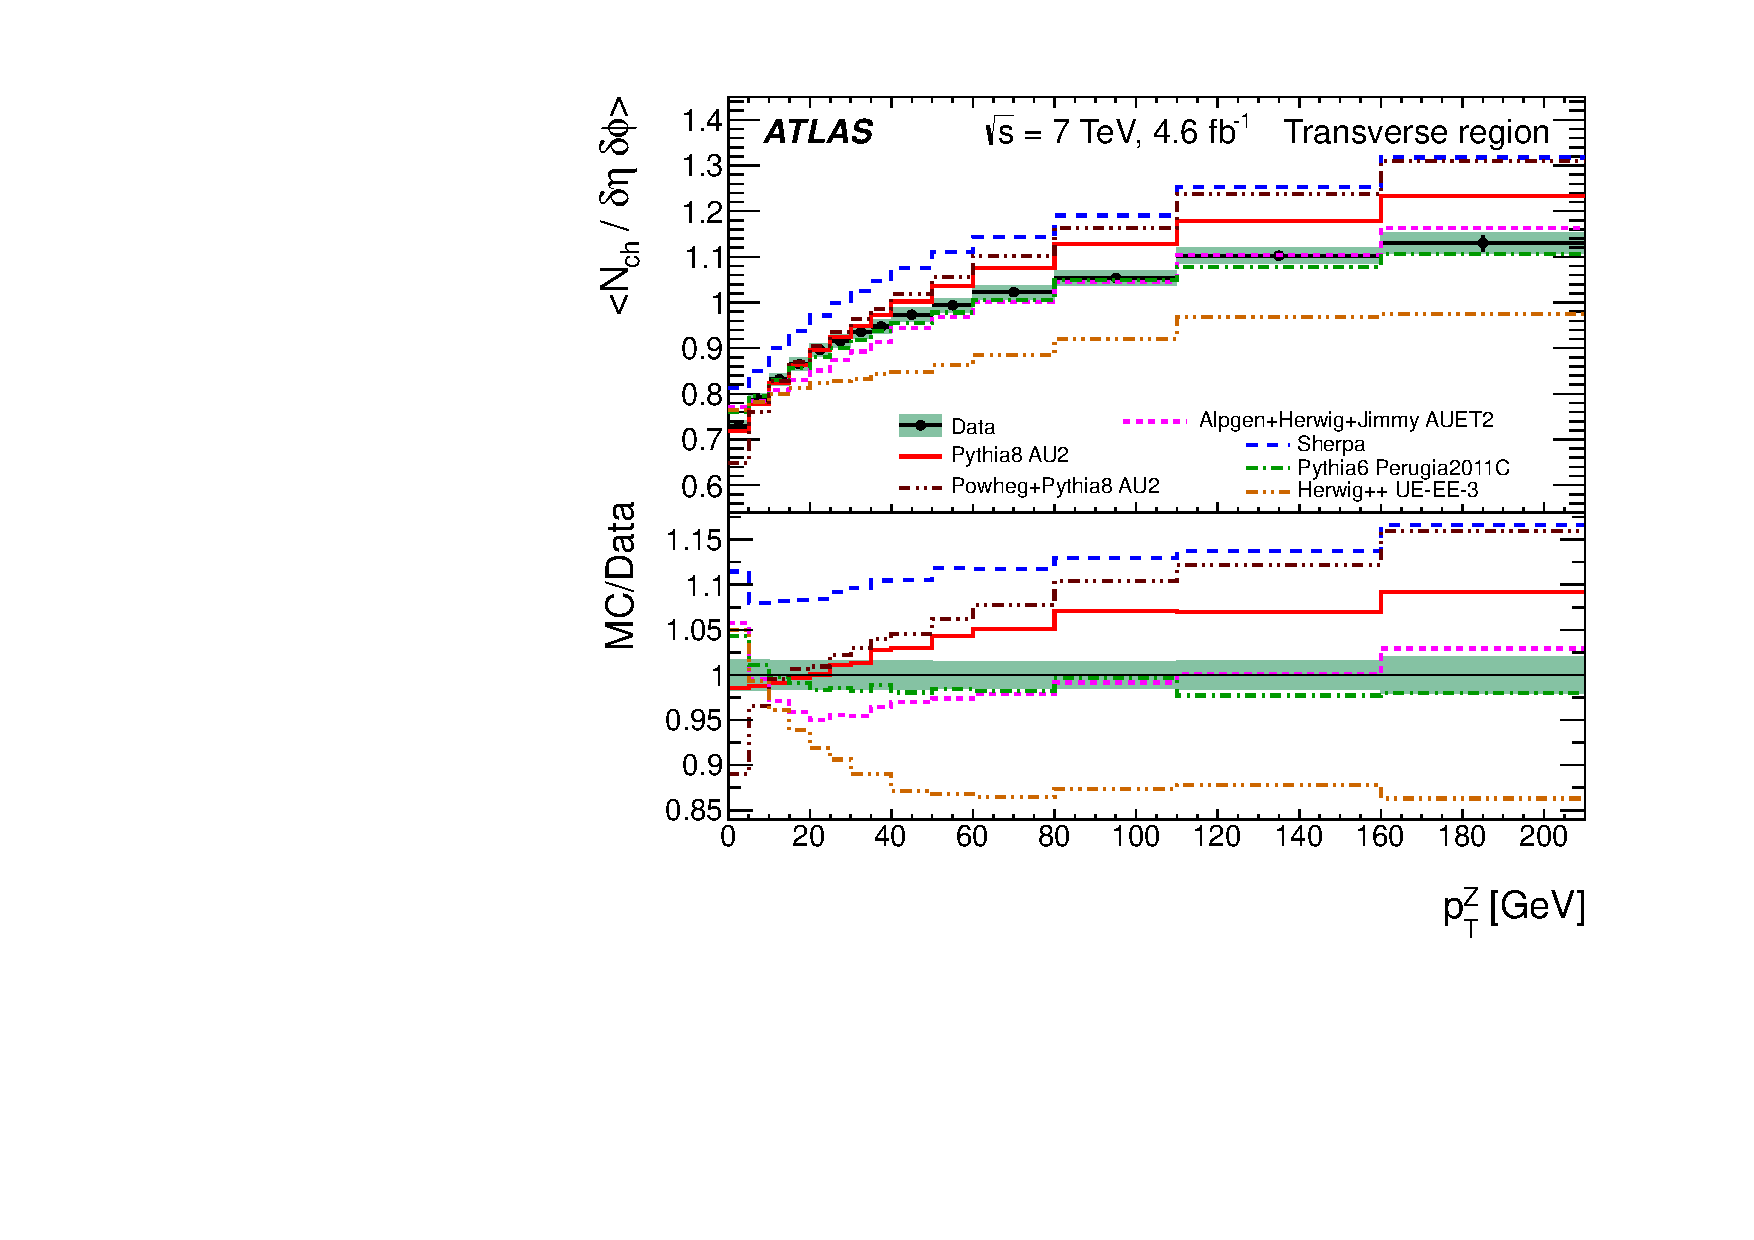
\includegraphics[width=0.48\textwidth]{figures/STDM-2011-42/fig_17b}
  \caption{Variables.}
  \label{fig:backgrounds-zue}
\end{figure}

\begin{figure}[tp]
  \centering
  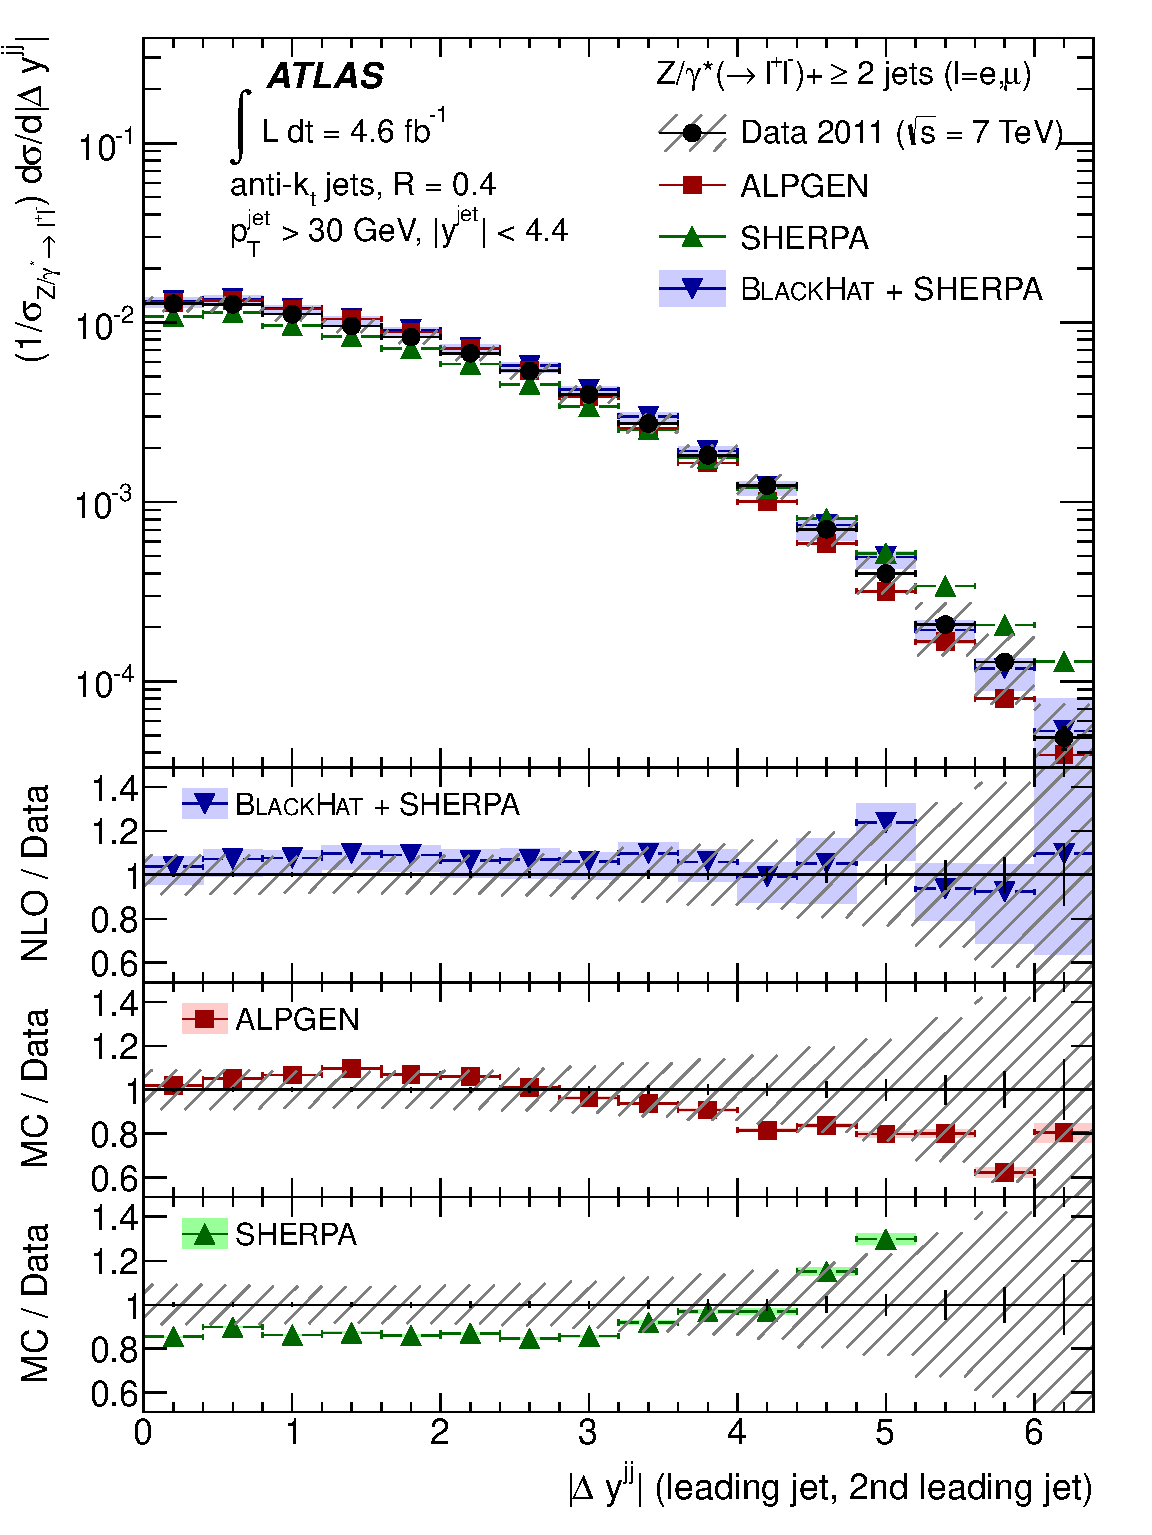
\includegraphics[width=0.48\textwidth]{figures/STDM-2012-04/fig_11a}
  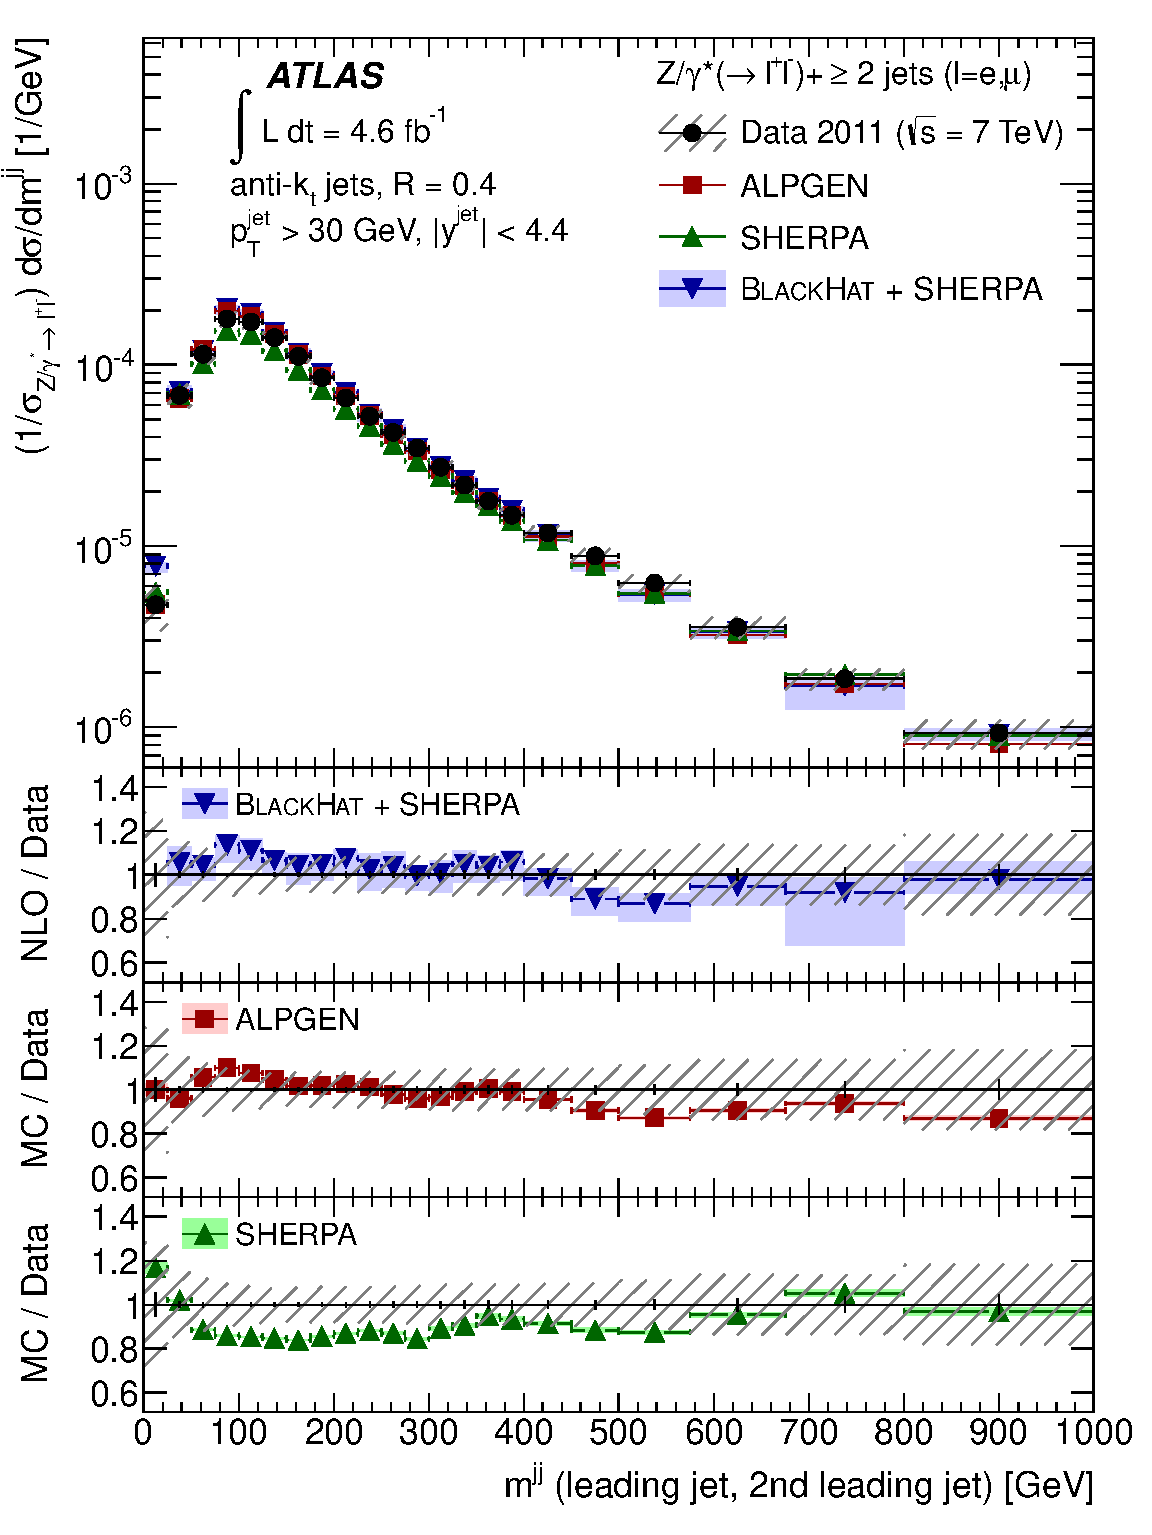
\includegraphics[width=0.48\textwidth]{figures/STDM-2012-04/fig_11b}
  \caption{Variables.}
  \label{fig:backgrounds-zjj}
\end{figure}

\begin{figure}[tp]
  \centering
  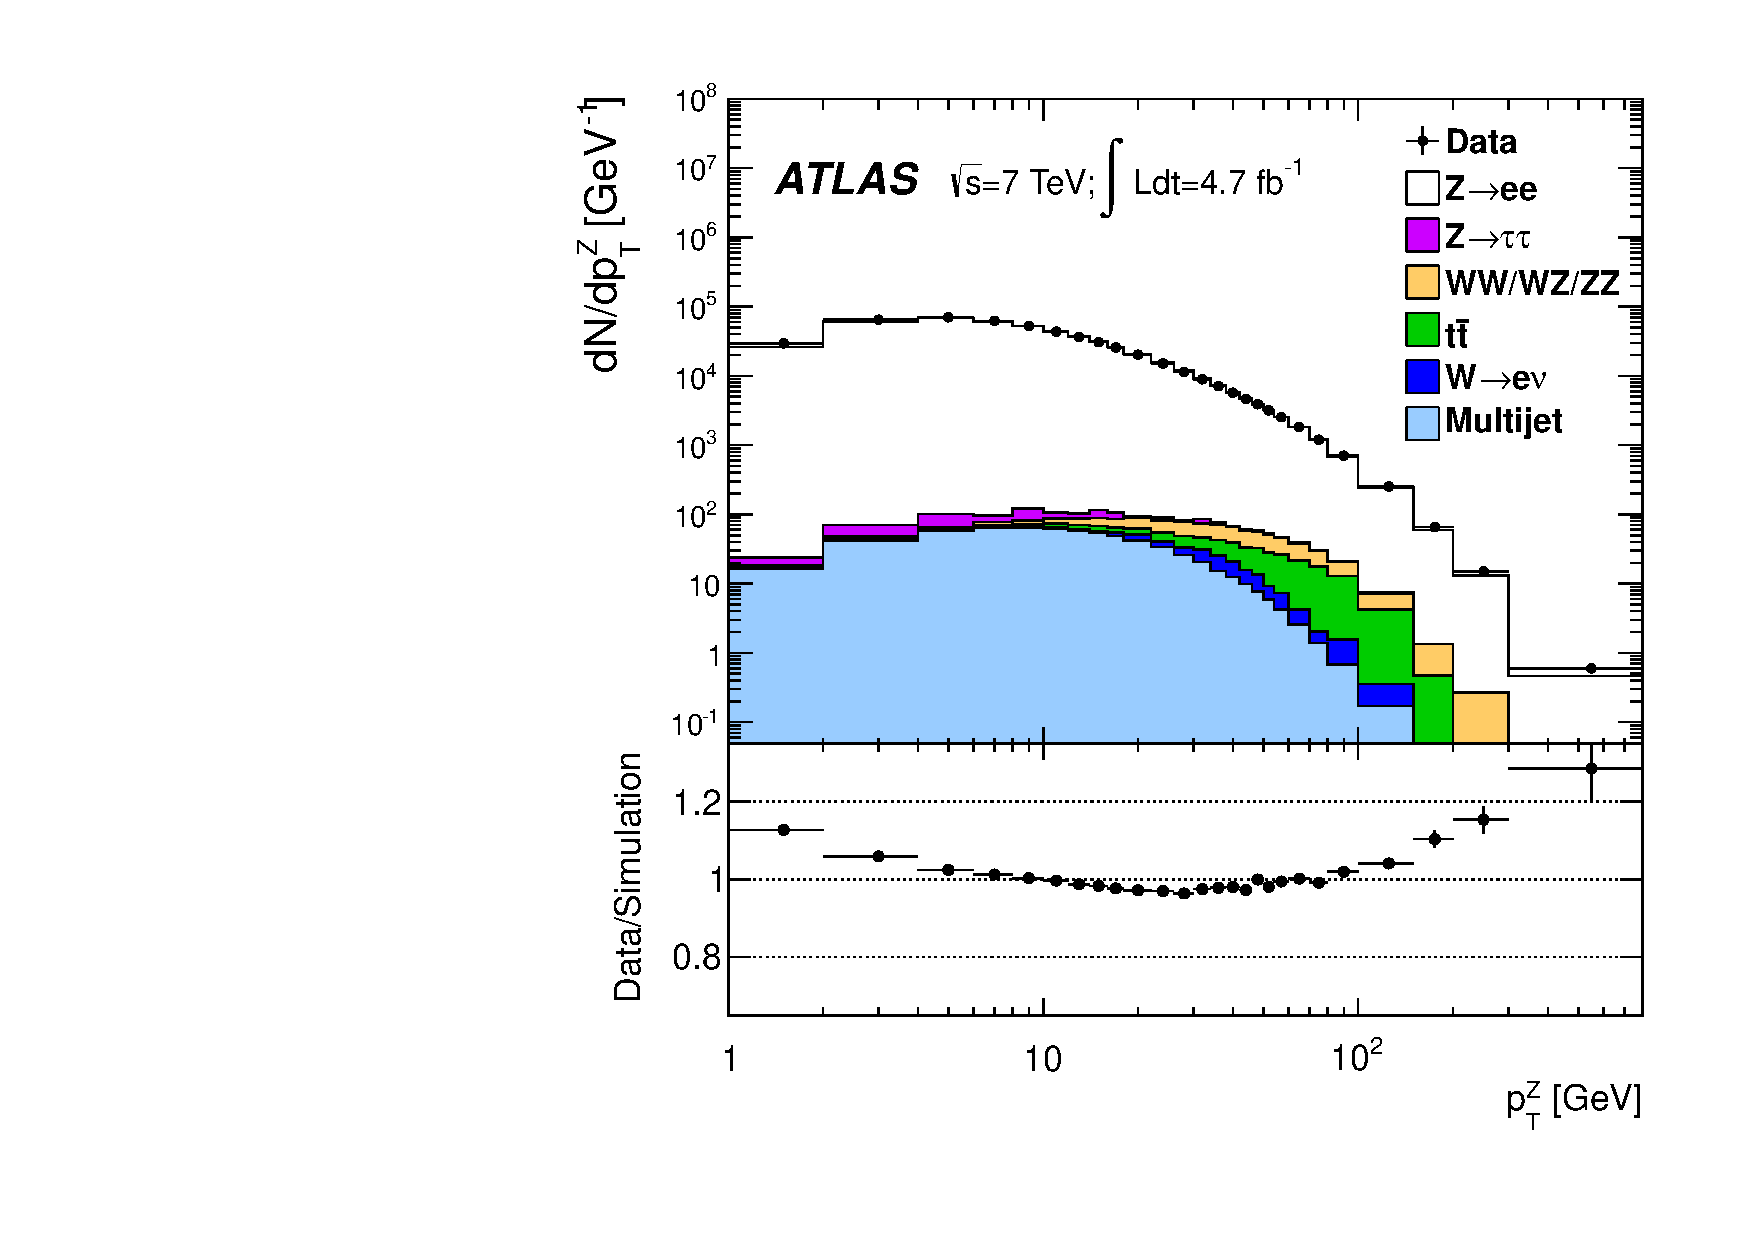
\includegraphics[width=0.48\textwidth]{figures/STDM-2012-23/fig_01a}
  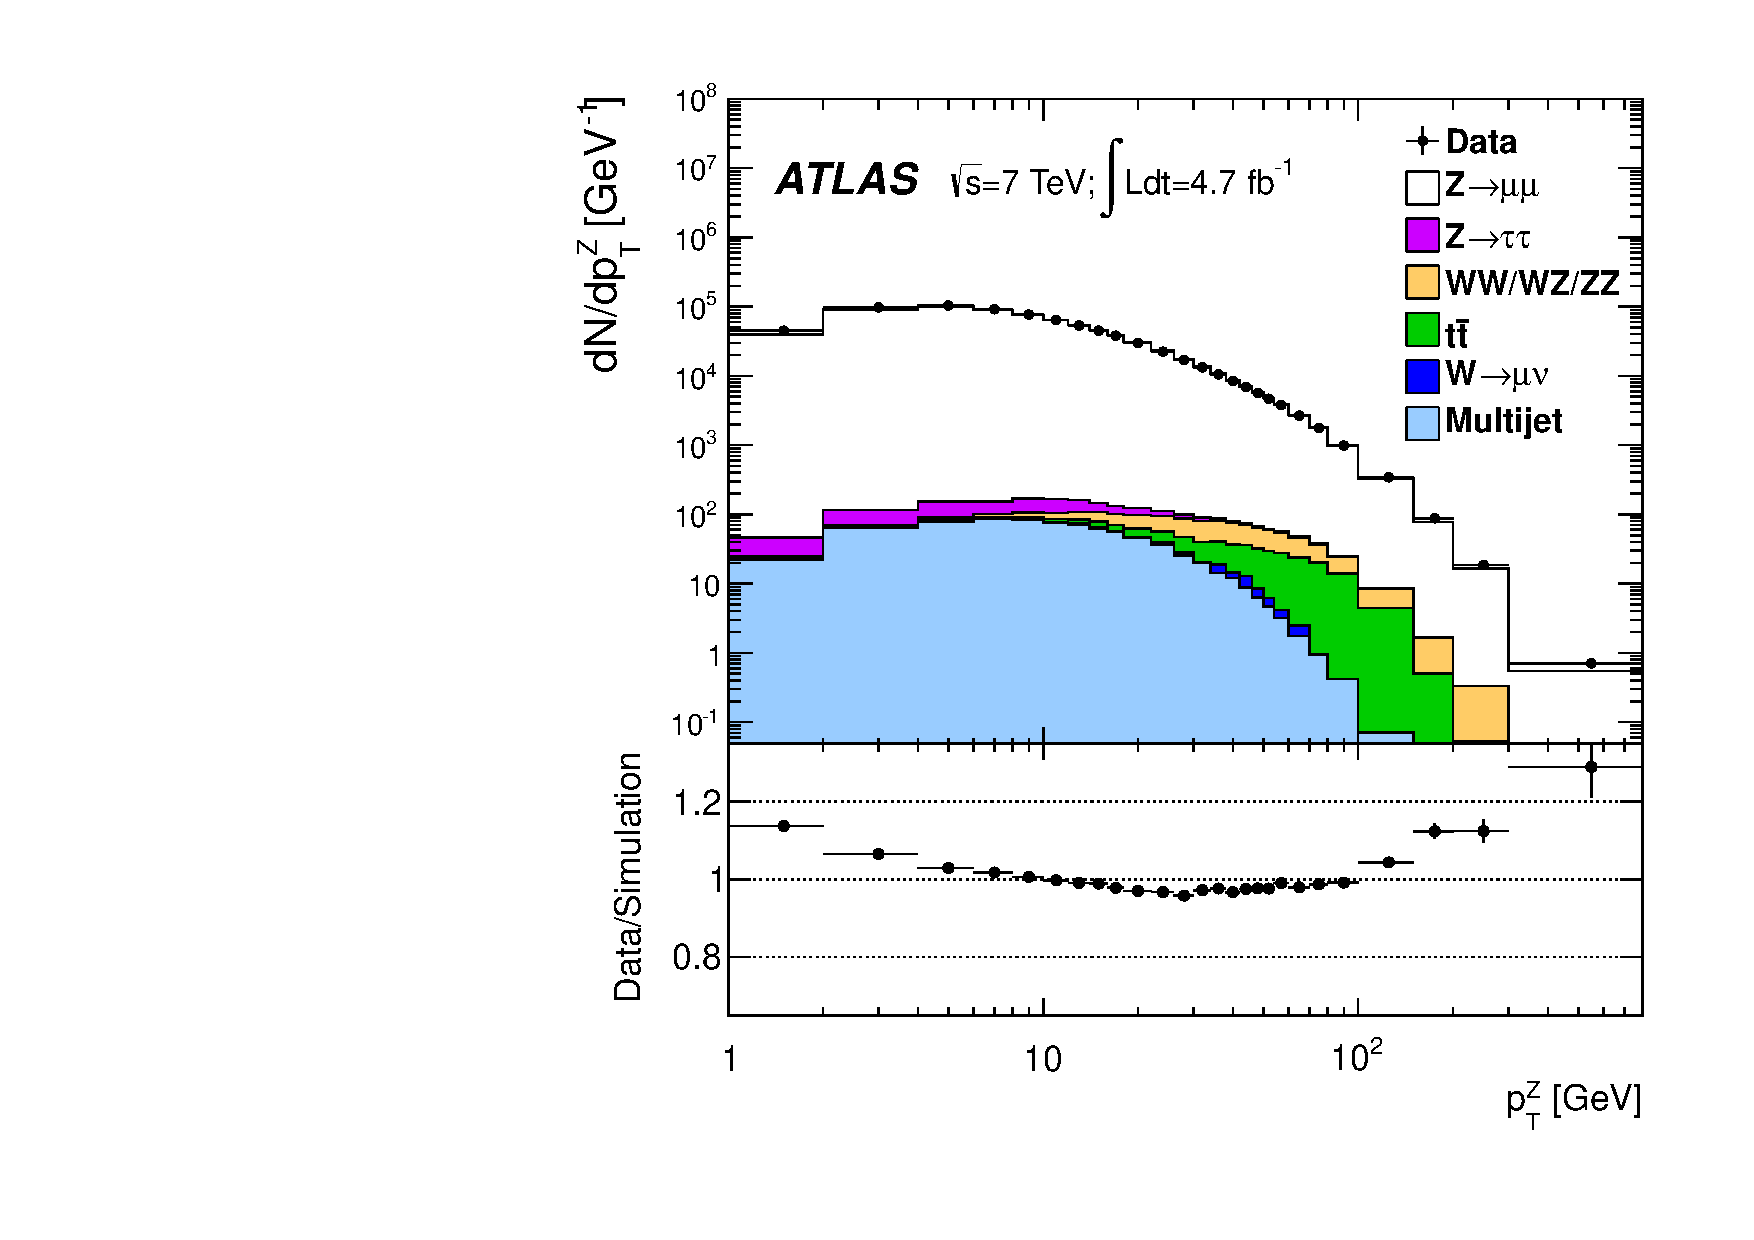
\includegraphics[width=0.48\textwidth]{figures/STDM-2012-23/fig_01b}
  \caption{Variables.}
  \label{fig:backgrounds-zpt}
\end{figure}

\begin{figure}[tp]
  \centering
  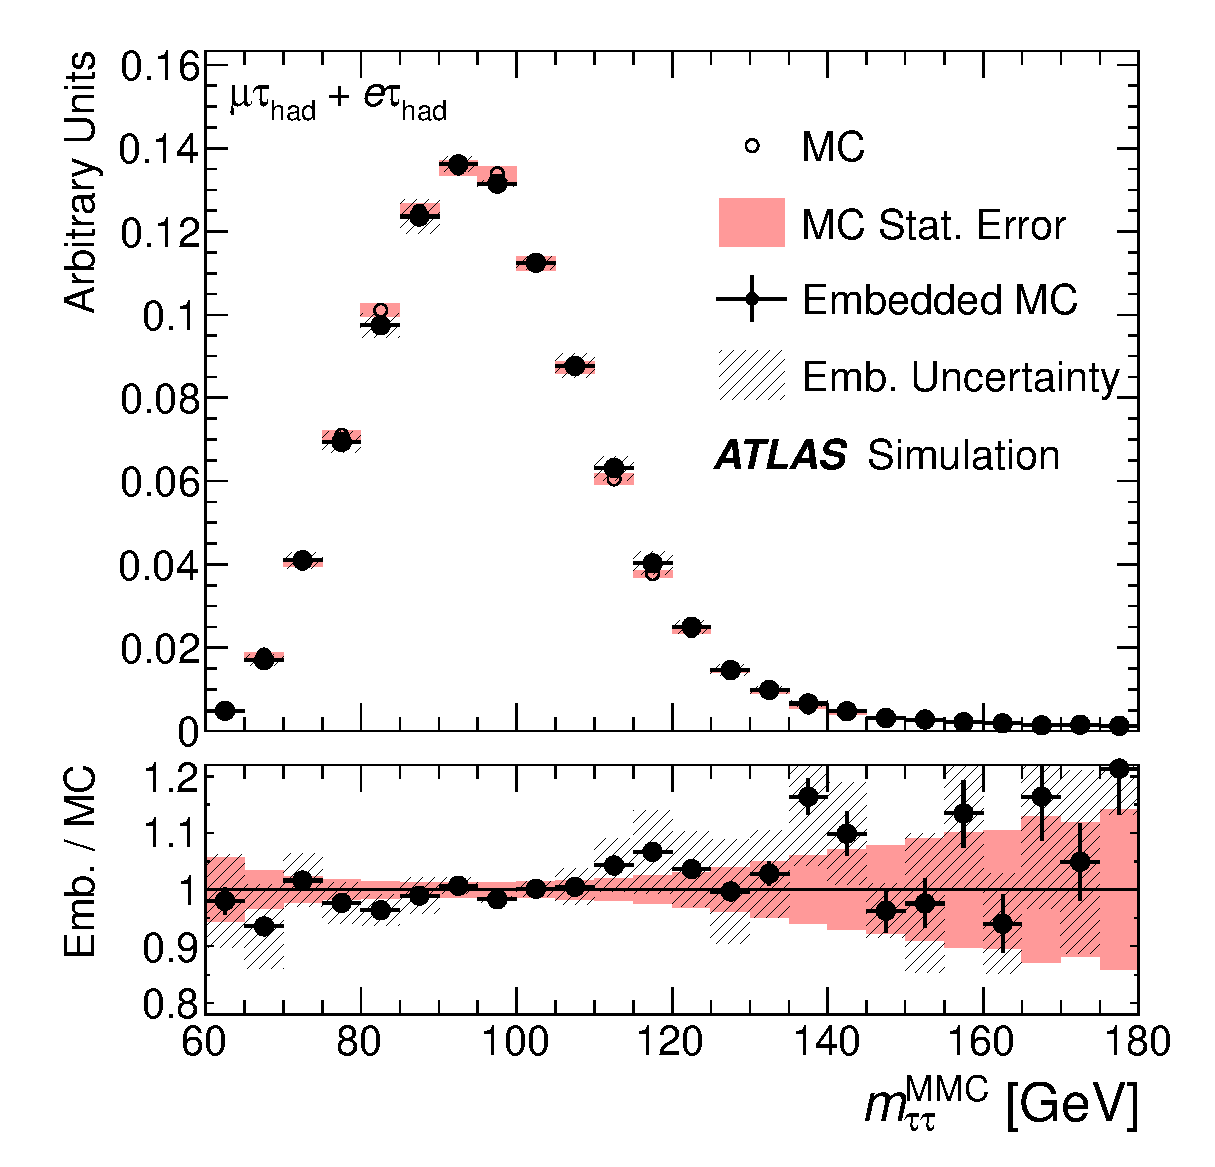
\includegraphics[width=0.48\textwidth]{figures/HIGG-2013-32/fig_03b}
  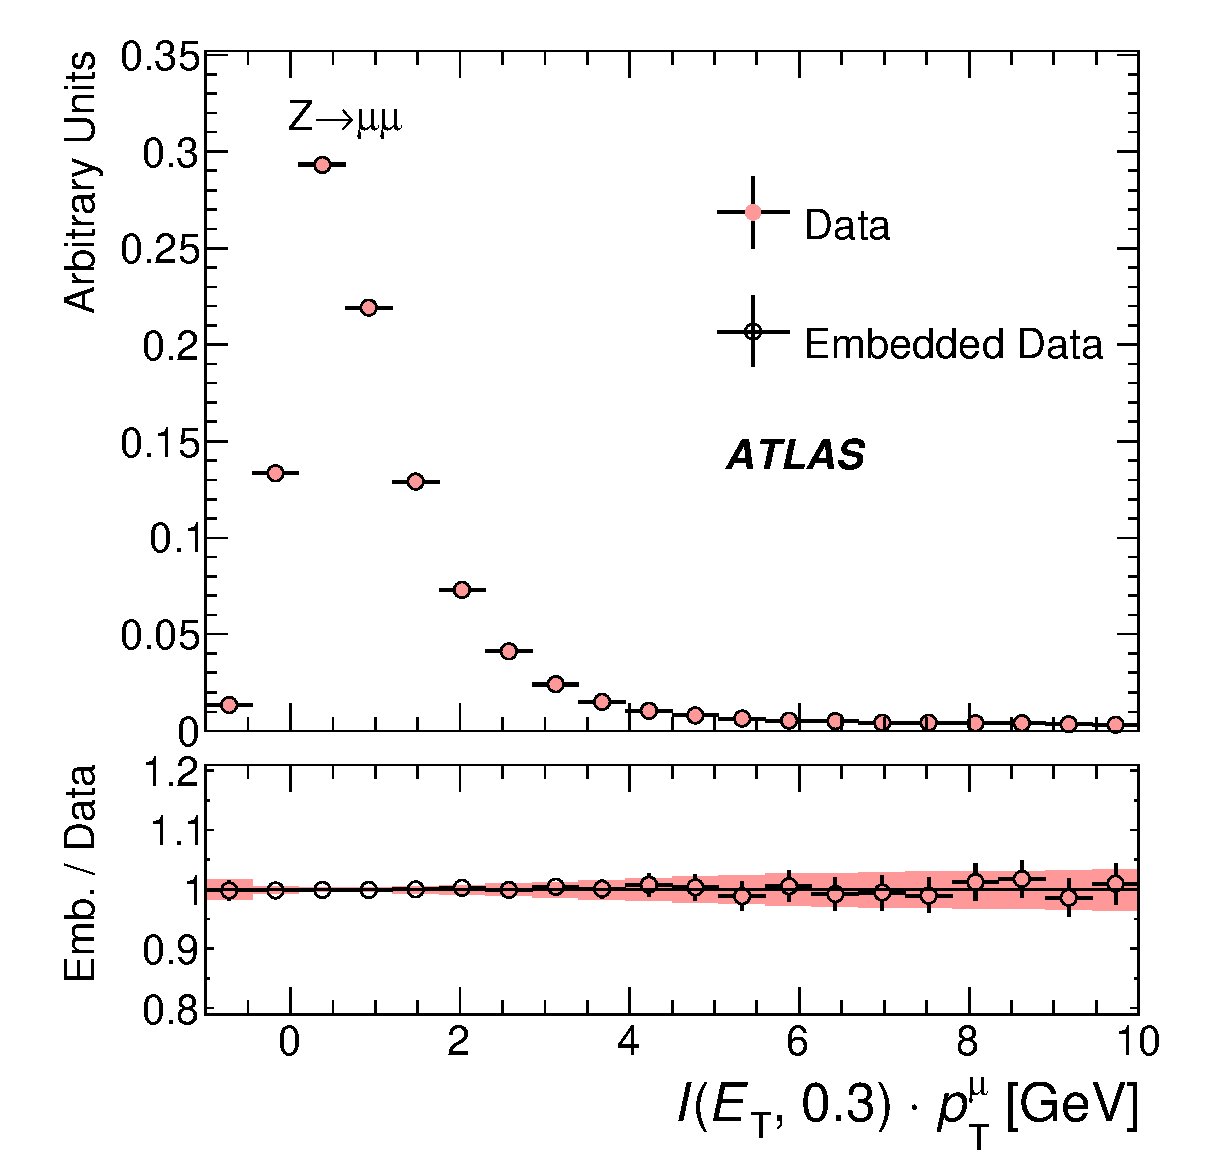
\includegraphics[width=0.48\textwidth]{figures/HIGG-2013-32/fig_03a}
  \caption{Variables.}
  \label{fig:backgrounds-embedding-valdation}
\end{figure}

\clearpage
\begin{figure}[tp]
  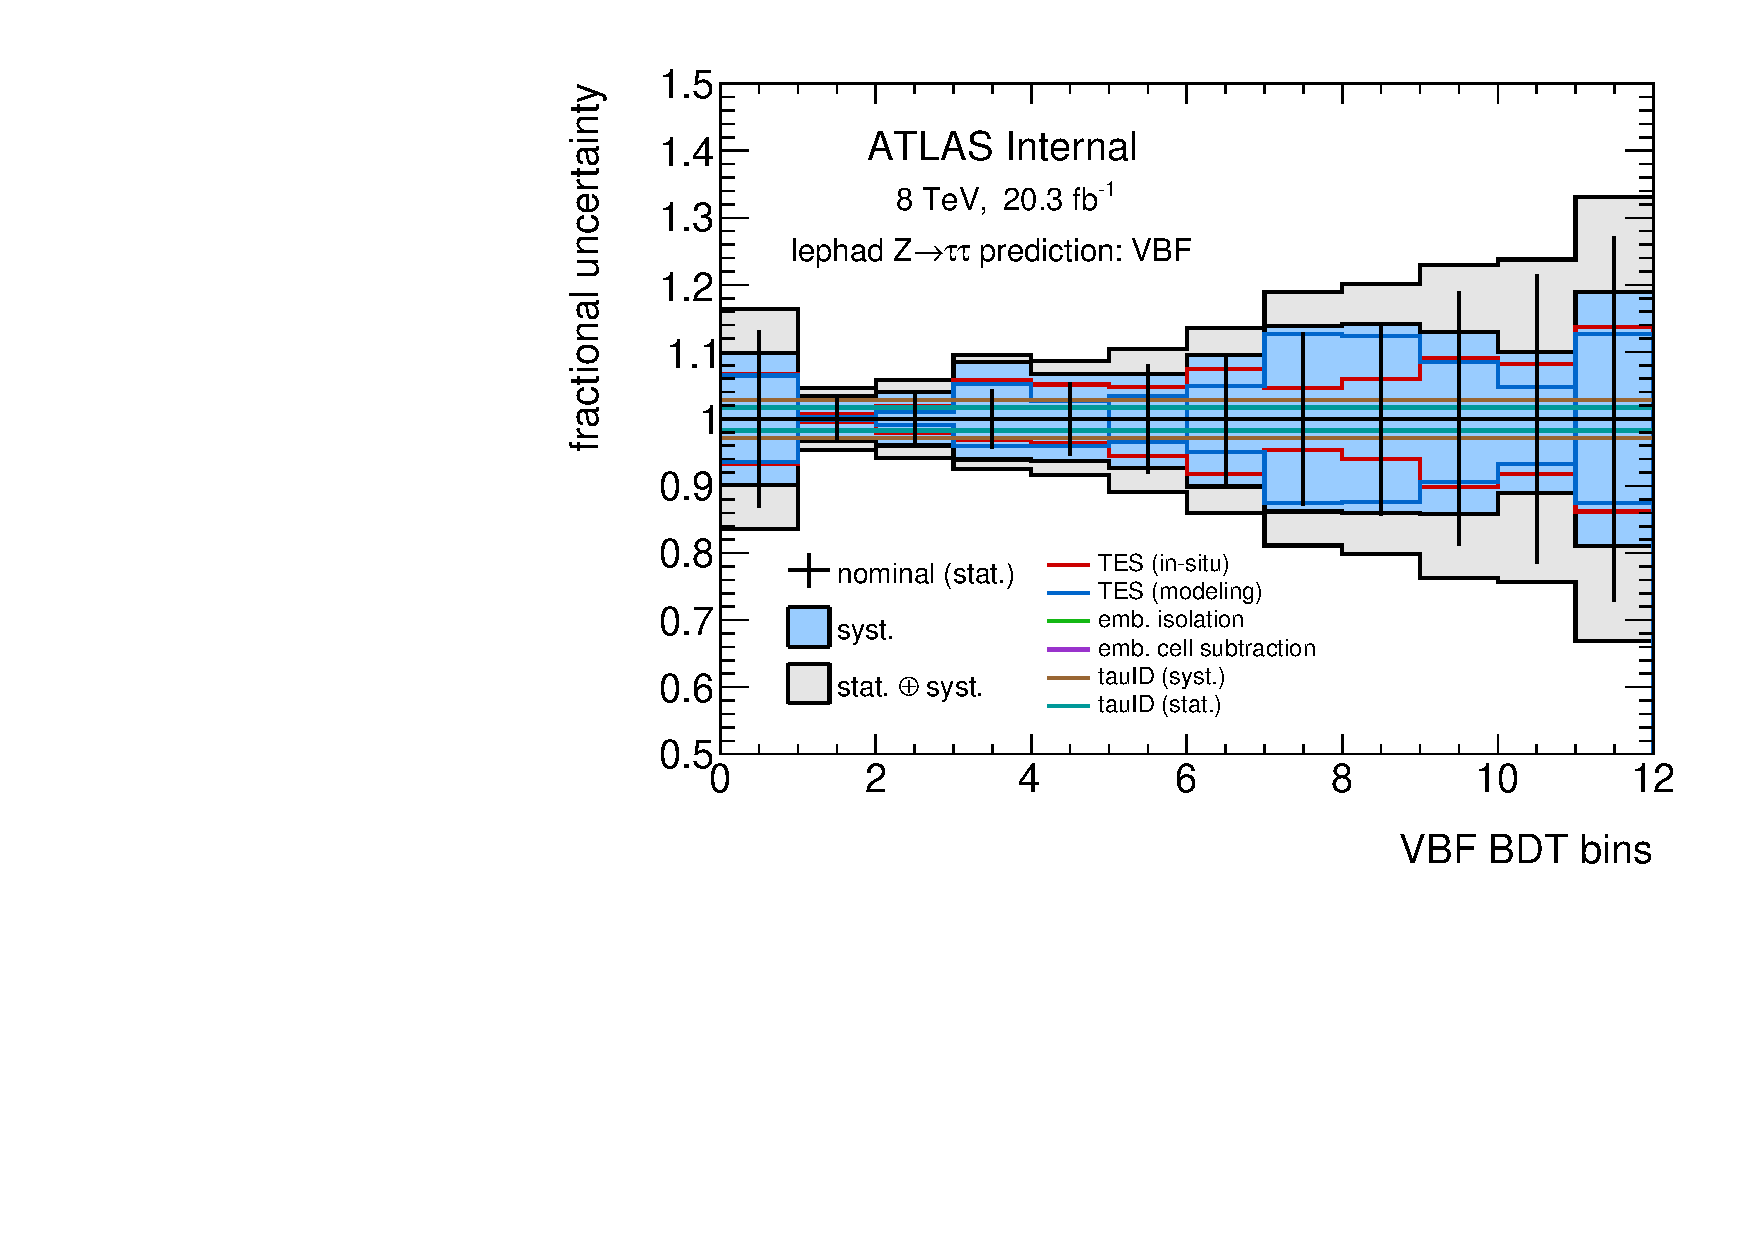
\includegraphics[width=0.90\textwidth]{figures/uncertainties/uncertainties_lephad_paper14_8TeV_Ztautau_VBF}
  \caption{Variables.}
  \label{fig:backgrounds-uncertainties-Ztautau}
\end{figure}

\clearpage
\section{$j \rightarrow \tauh$ mis-identification}
\label{sec:backgrounds-misid}

\begin{figure}[tp]
  \centering
  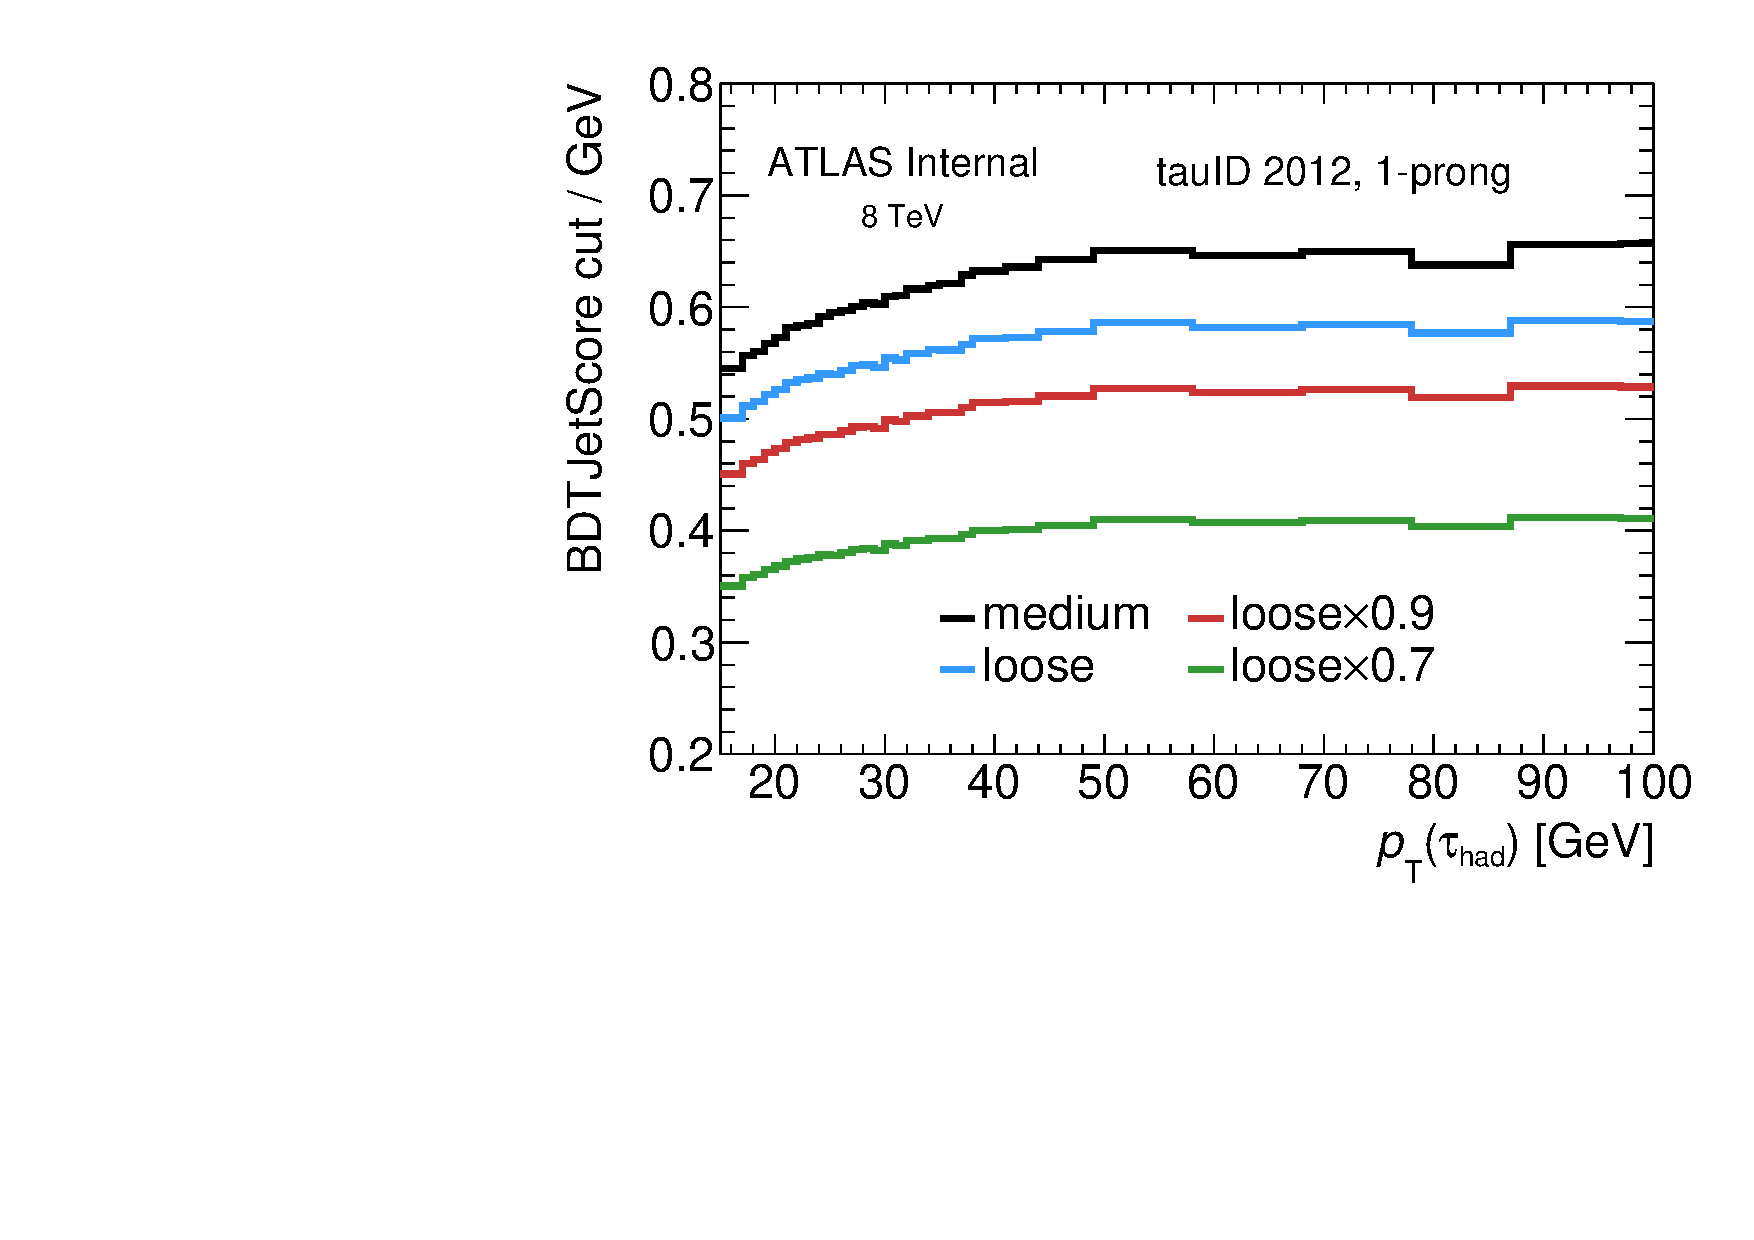
\includegraphics[width=0.48\textwidth]{figures/backgrounds/jetBDT-1p}
  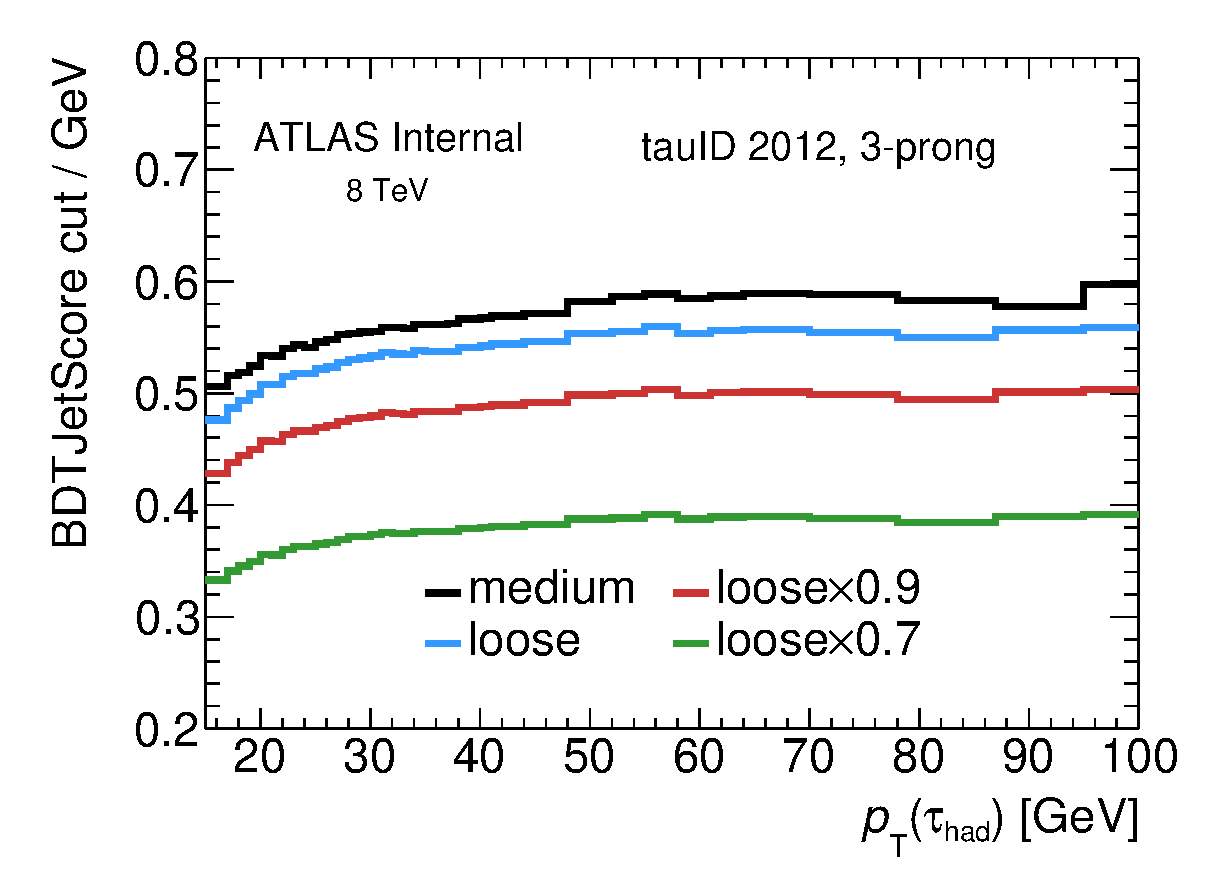
\includegraphics[width=0.48\textwidth]{figures/backgrounds/jetBDT-3p}
  \caption{Variables.}
  \label{fig:backgrounds-workingpoints}
\end{figure}

\begin{figure}[tp]
  \centering
  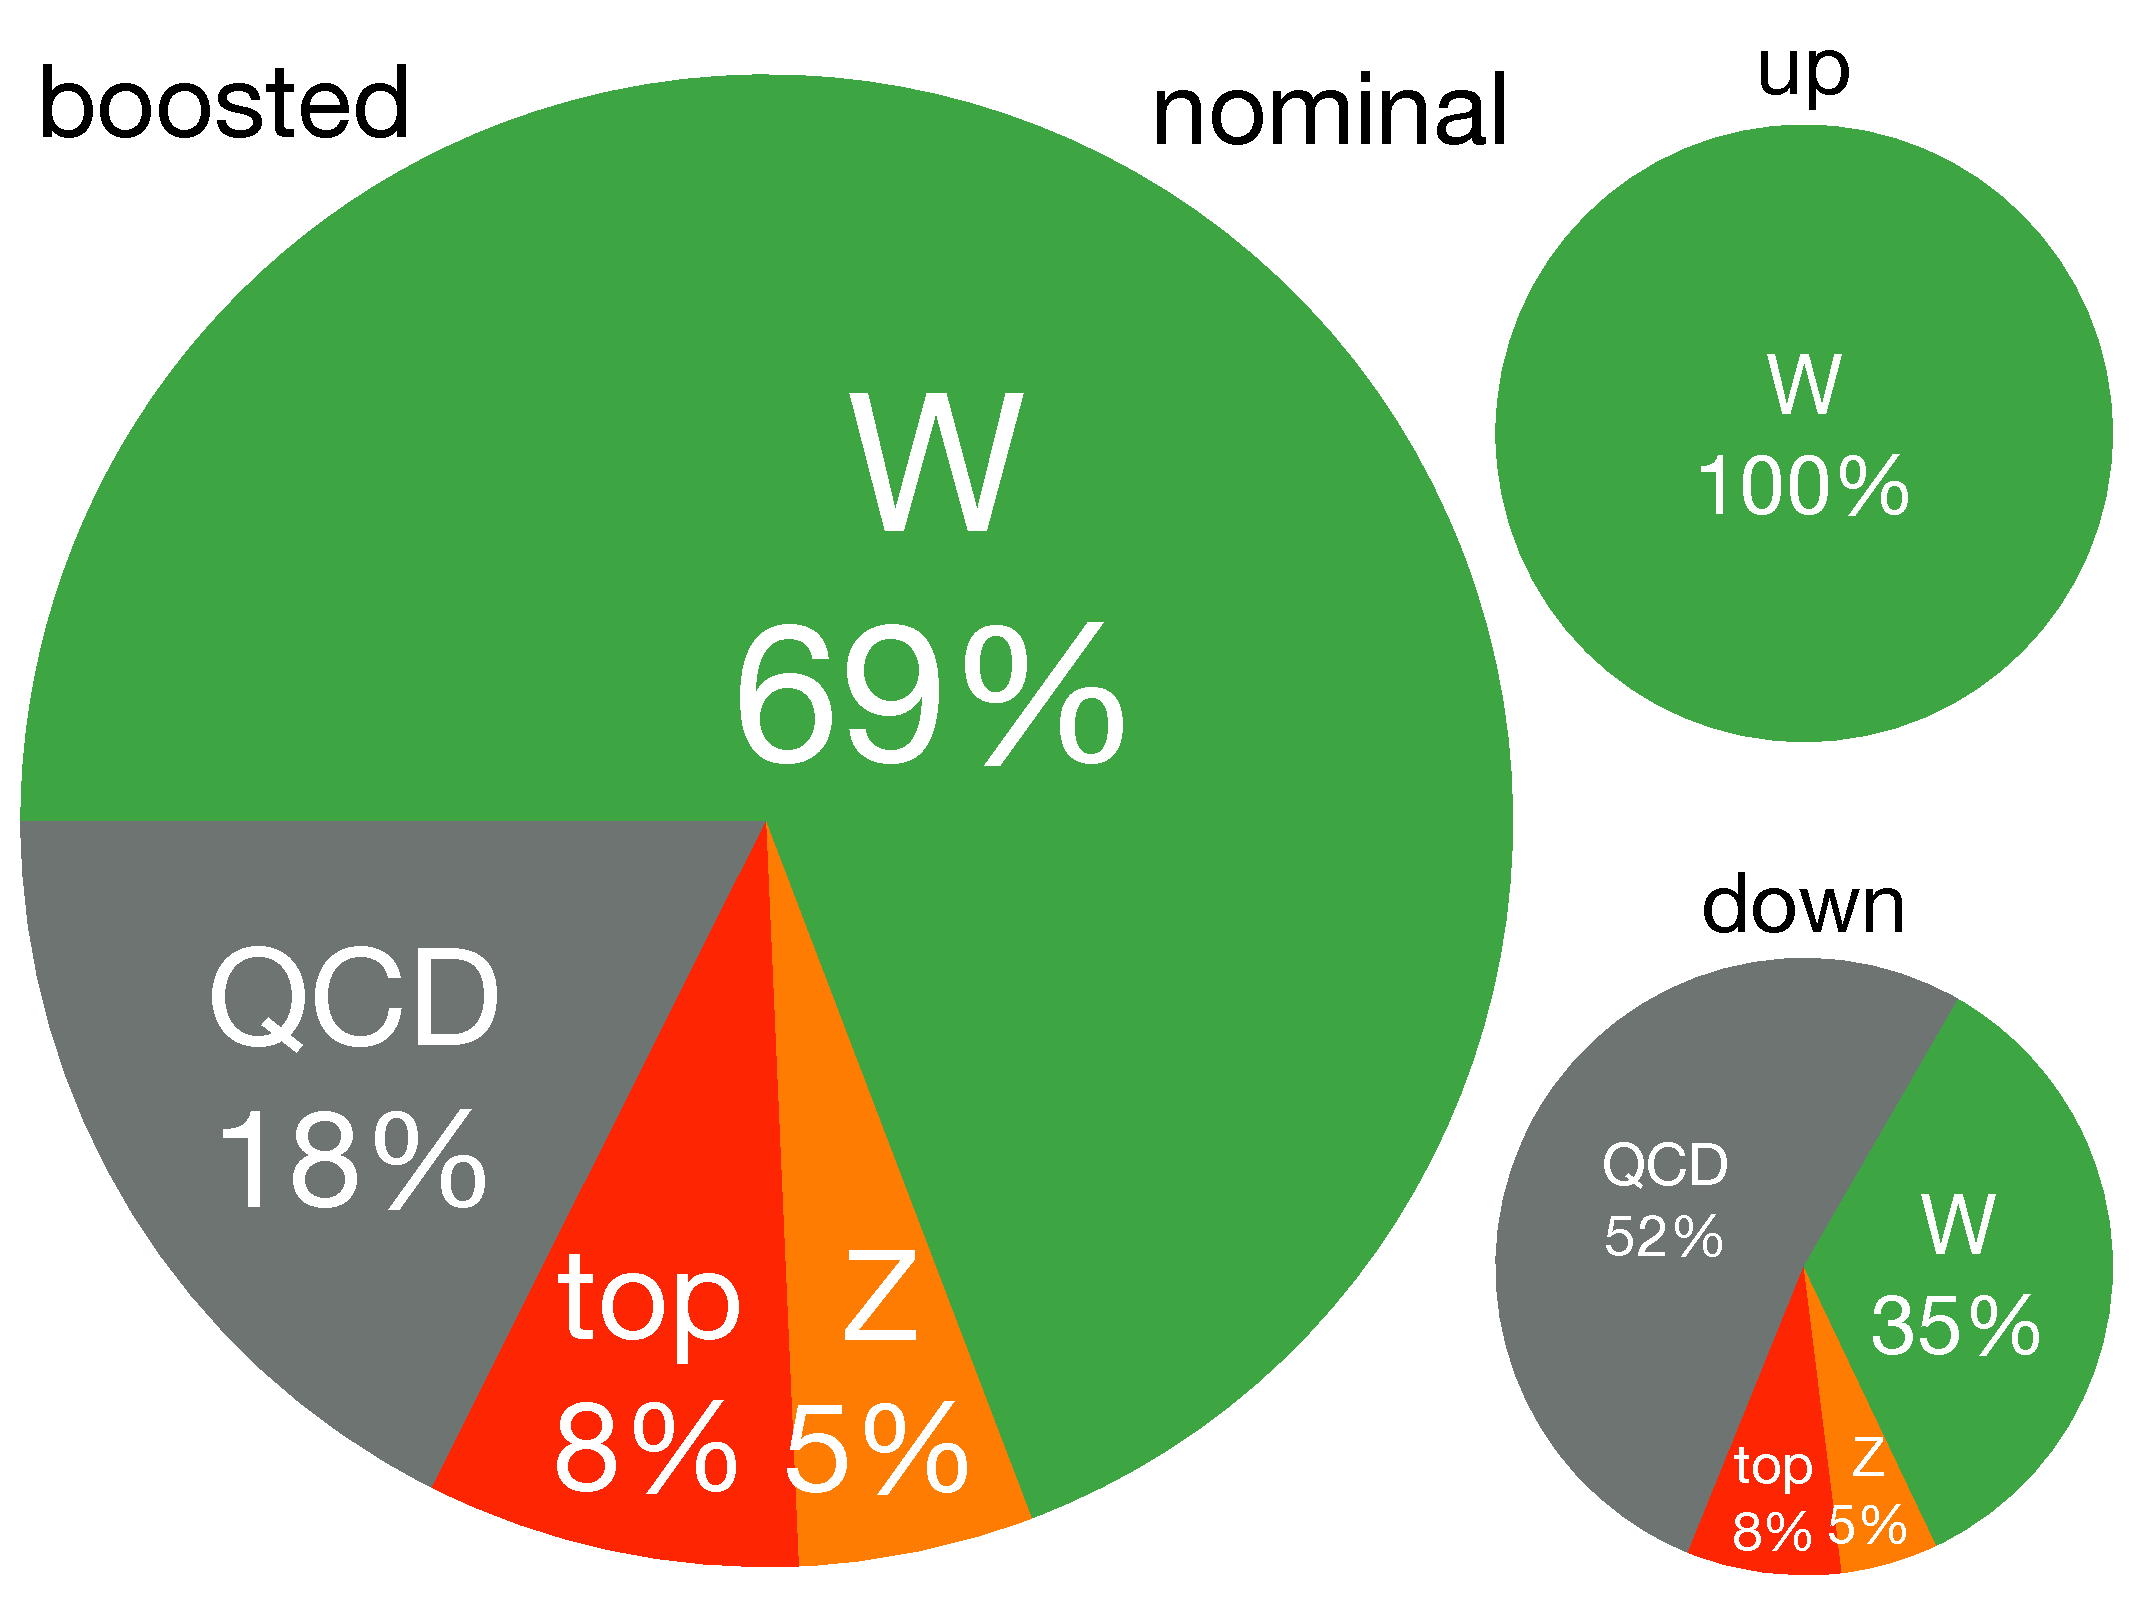
\includegraphics[width=0.90\textwidth]{figures/backgrounds/rx-boost}
  \caption{Variables.}
  \label{fig:backgrounds-rx-boost}
\end{figure}

\begin{figure}[tp]
  \centering
  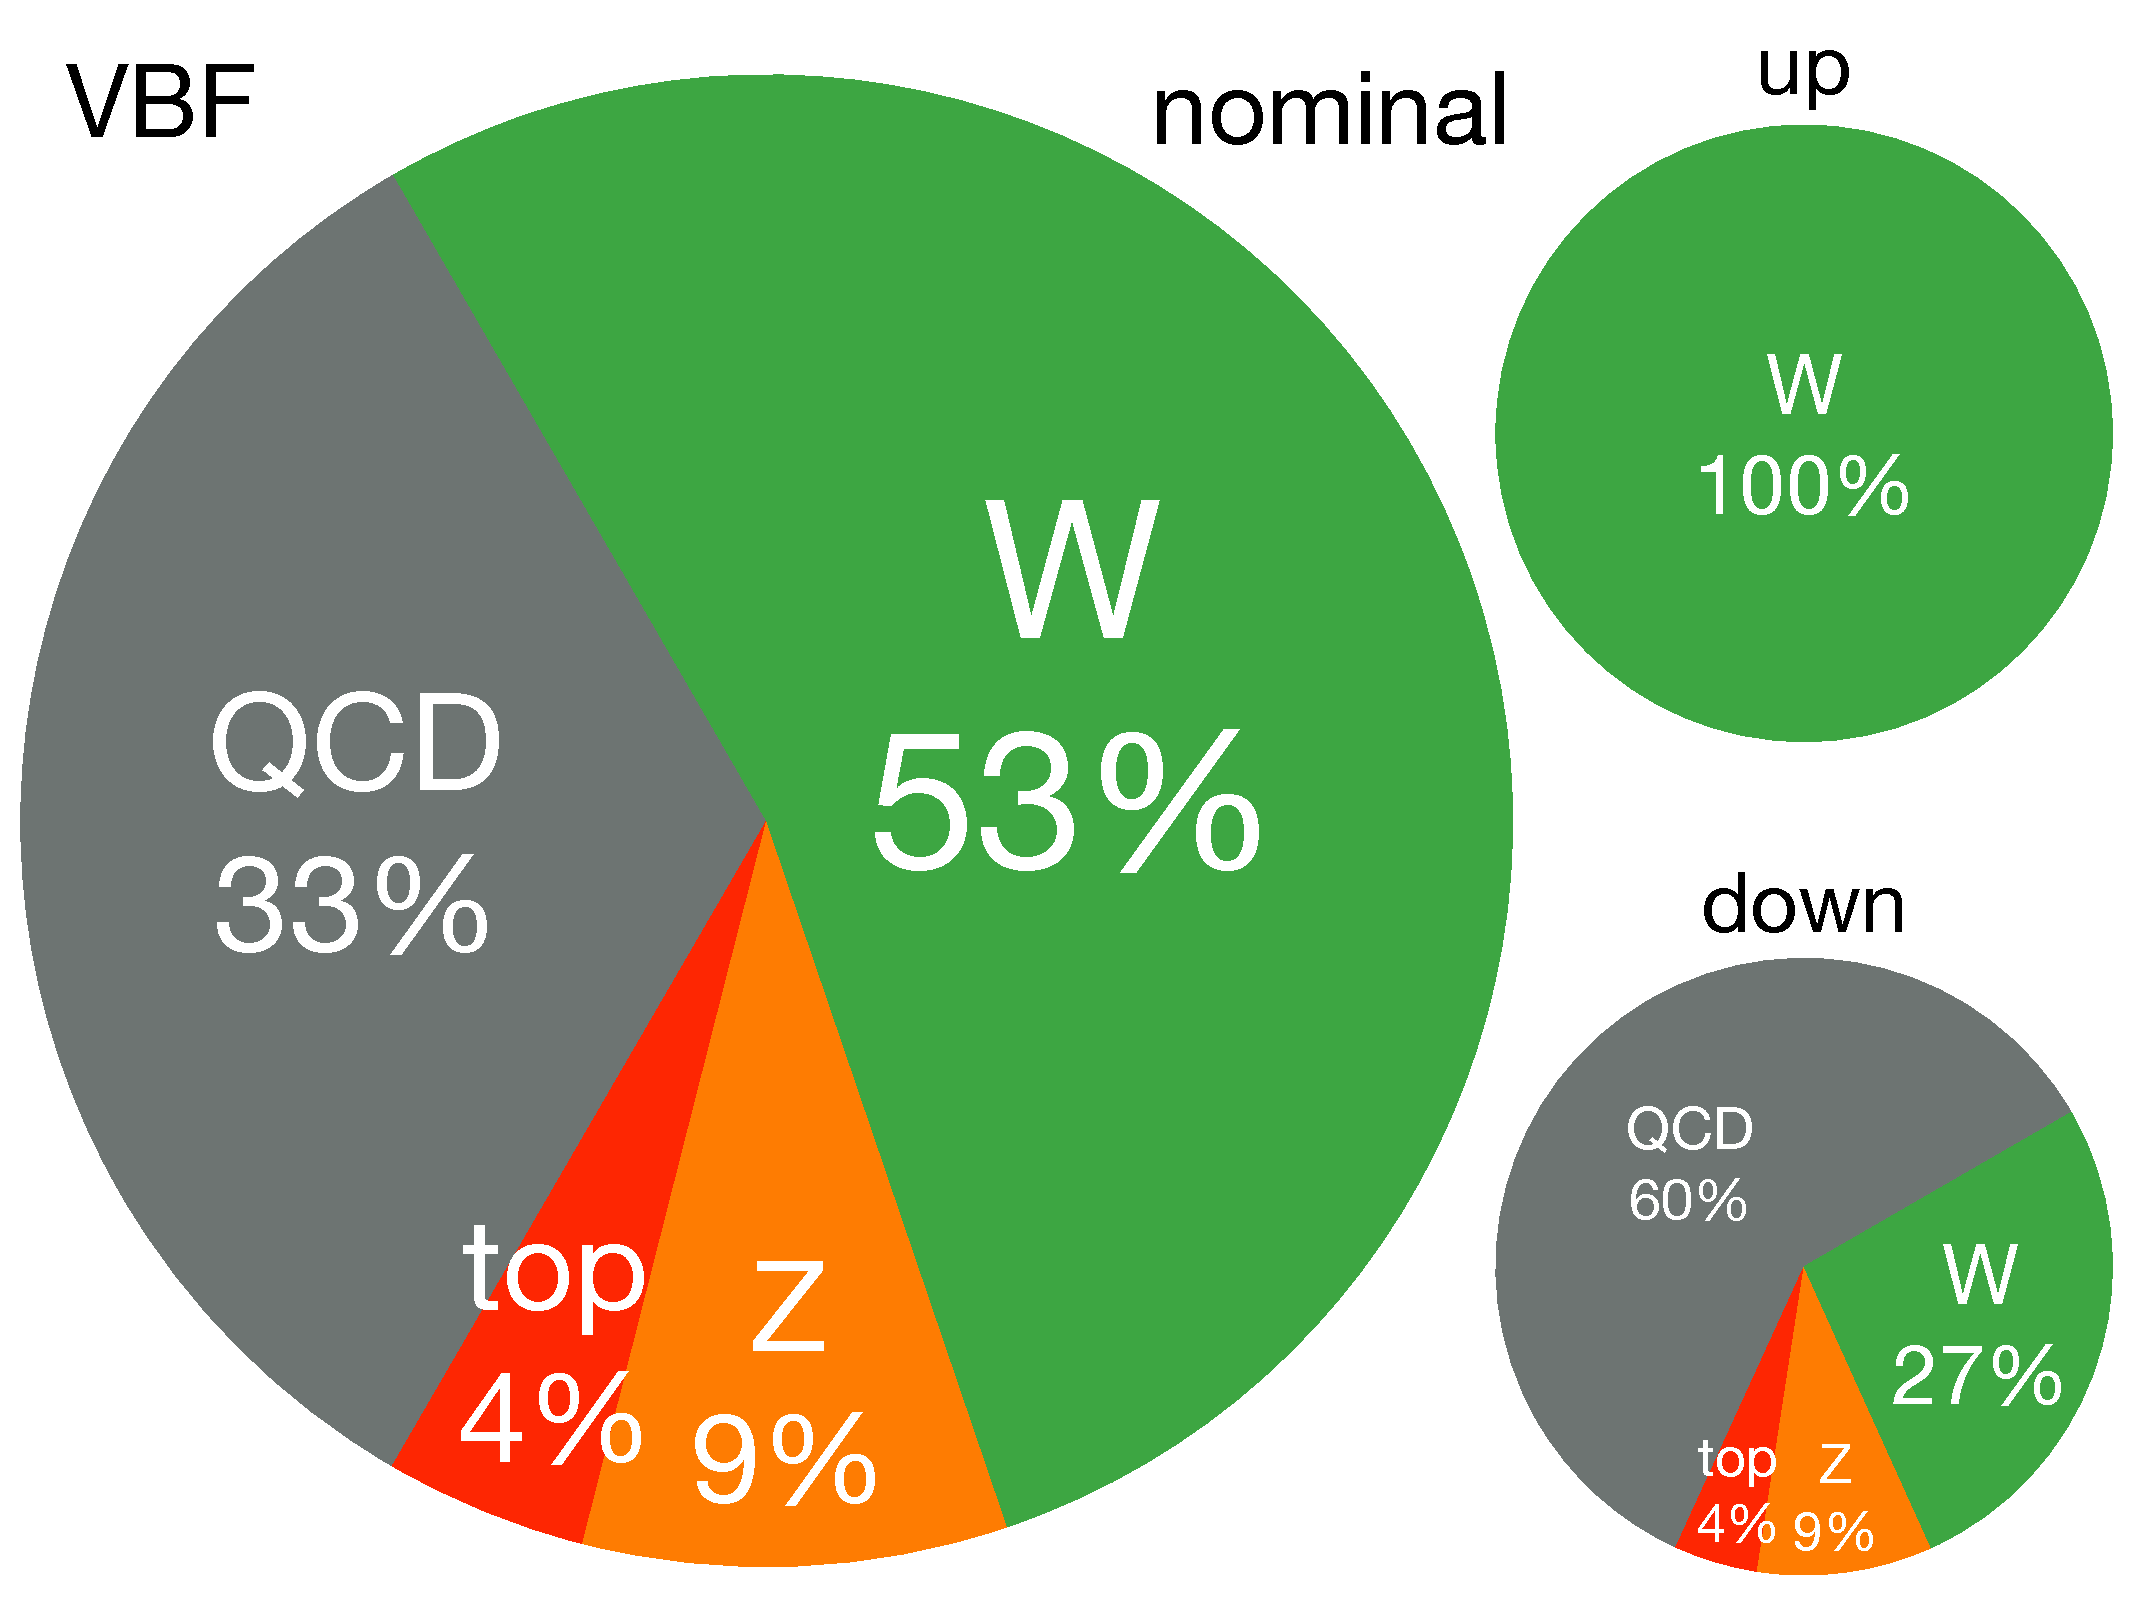
\includegraphics[width=0.90\textwidth]{figures/backgrounds/rx-vbf}
  \caption{Variables.}
  \label{fig:backgrounds-rx-vbf}
\end{figure}

\clearpage

\begin{figure}[tp]
  \centering
  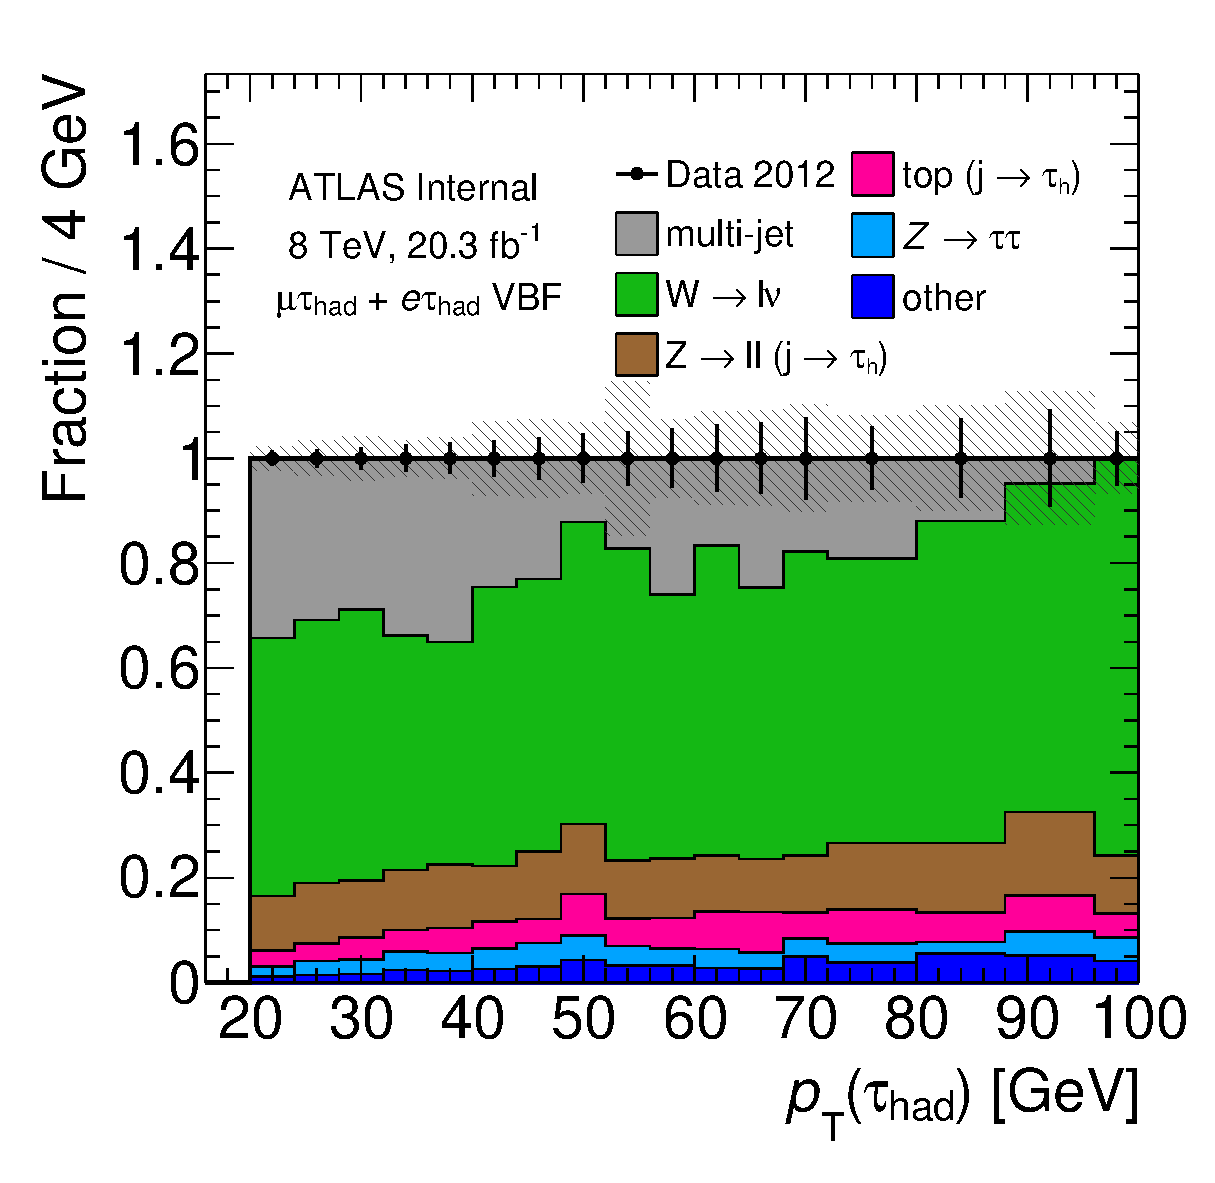
\includegraphics[width=0.32\textwidth]{figures/rx/vbf-mvaSR/tau-pt}
  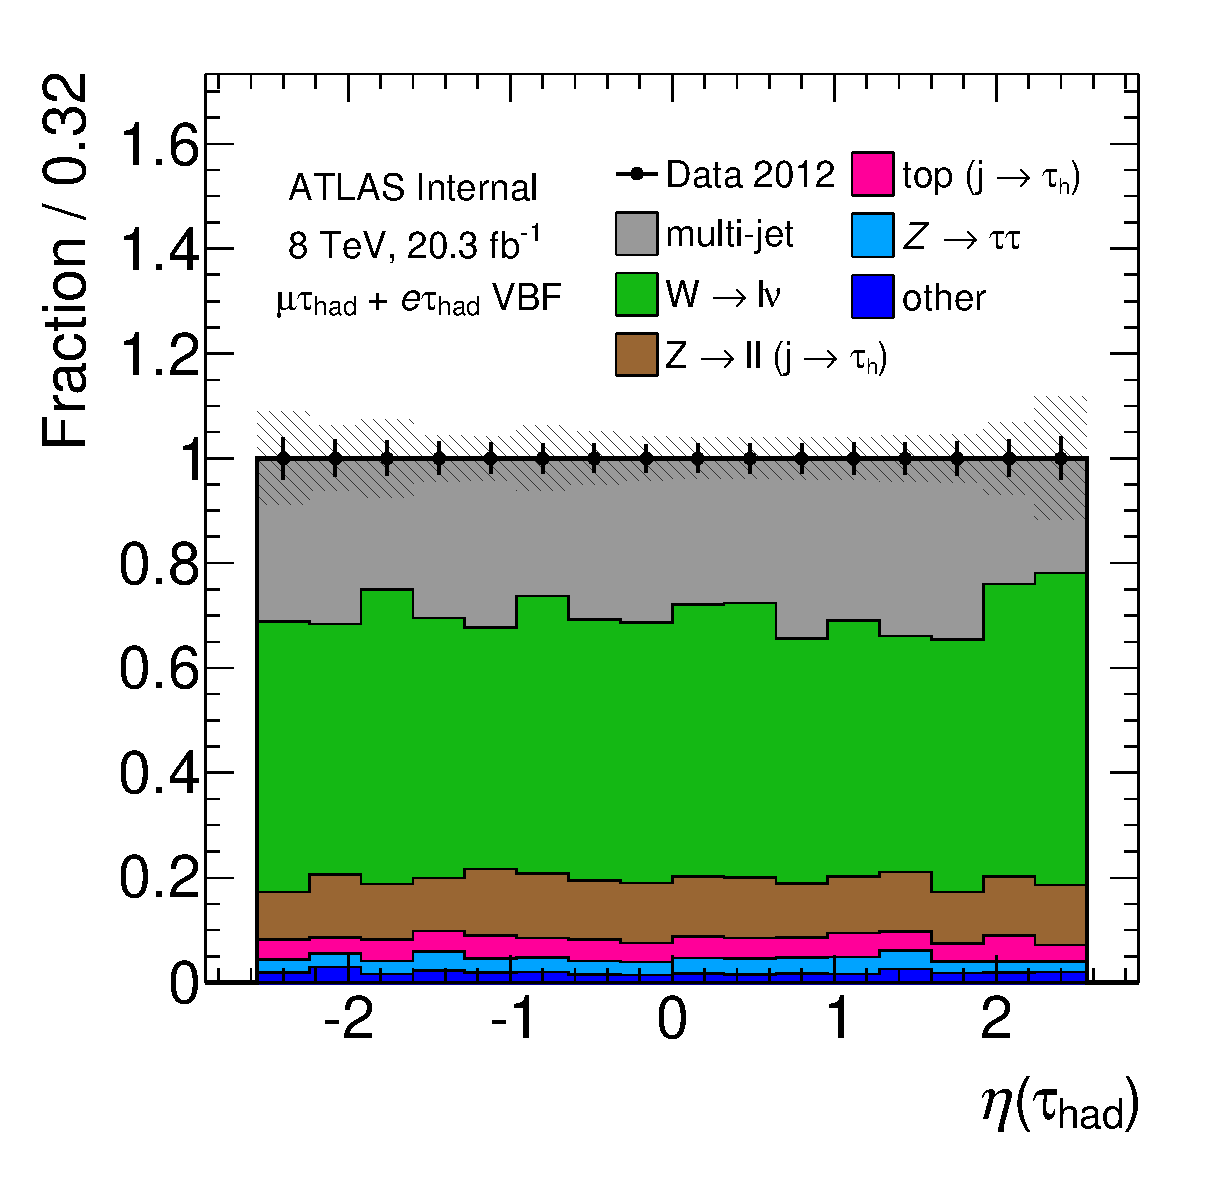
\includegraphics[width=0.32\textwidth]{figures/rx/vbf-mvaSR/tau-eta}
  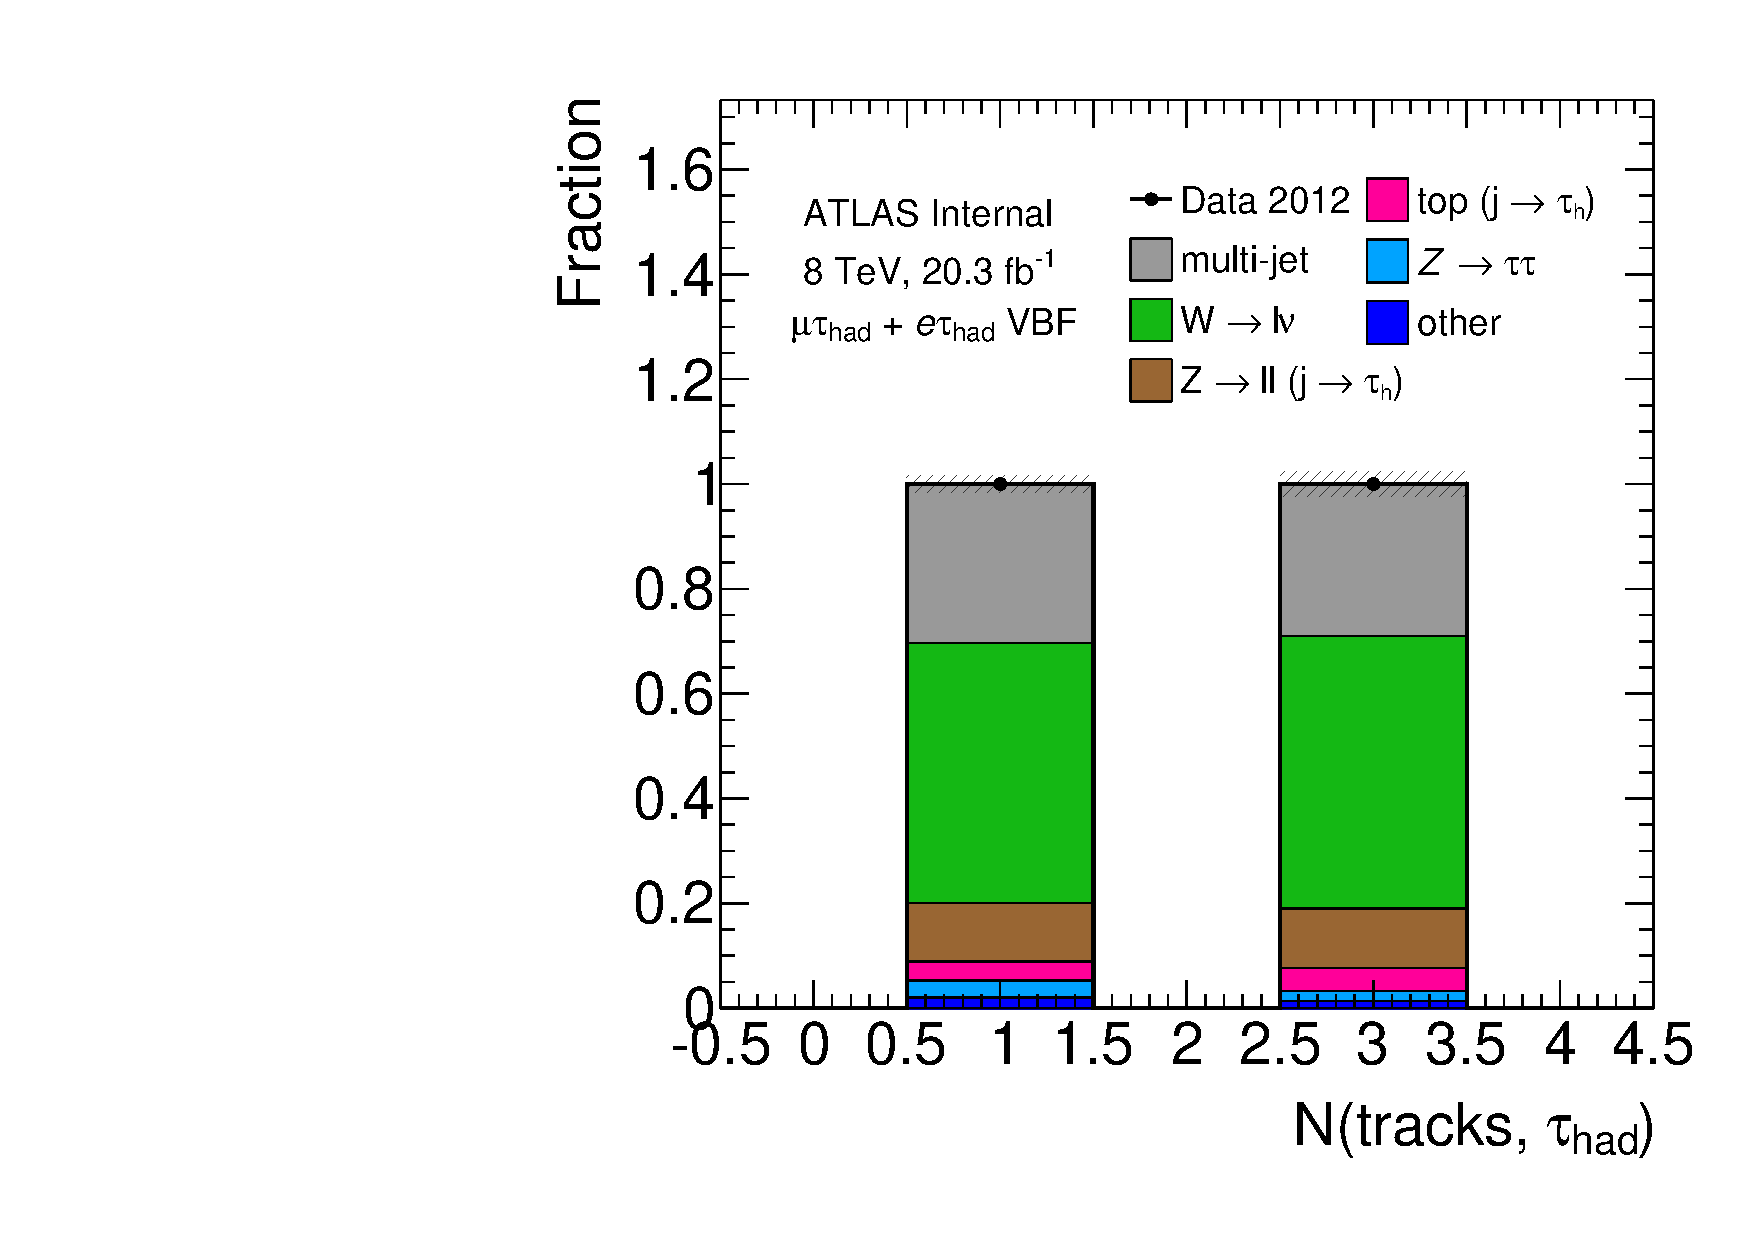
\includegraphics[width=0.32\textwidth]{figures/rx/vbf-mvaSR/tau-numTrack}
  % --------------
  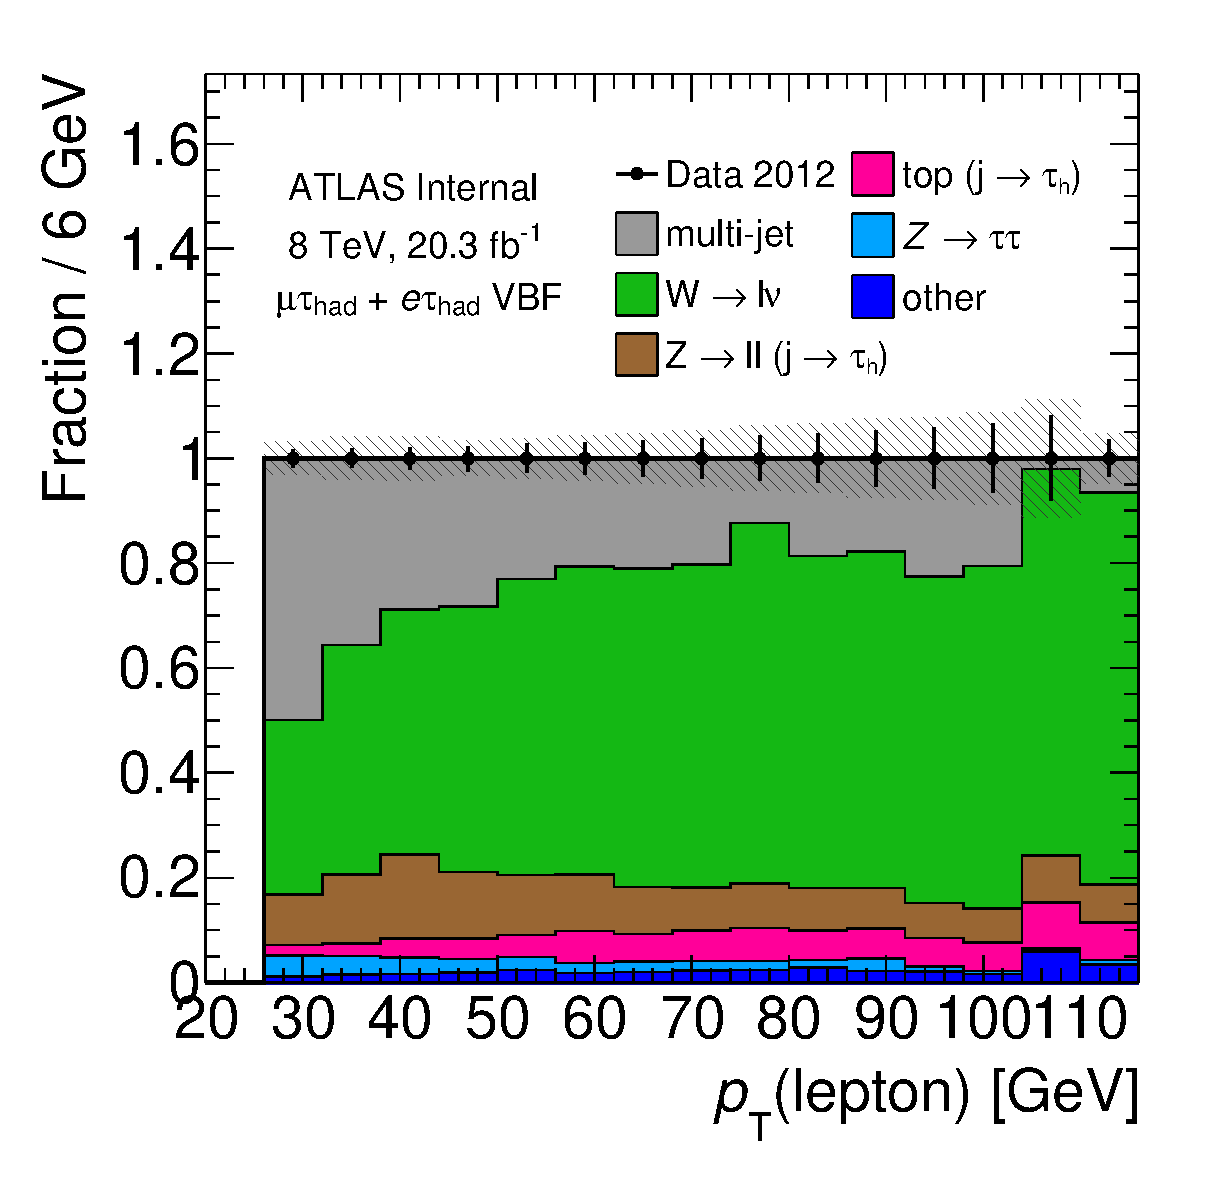
\includegraphics[width=0.32\textwidth]{figures/rx/vbf-mvaSR/lep-pt-hi}
  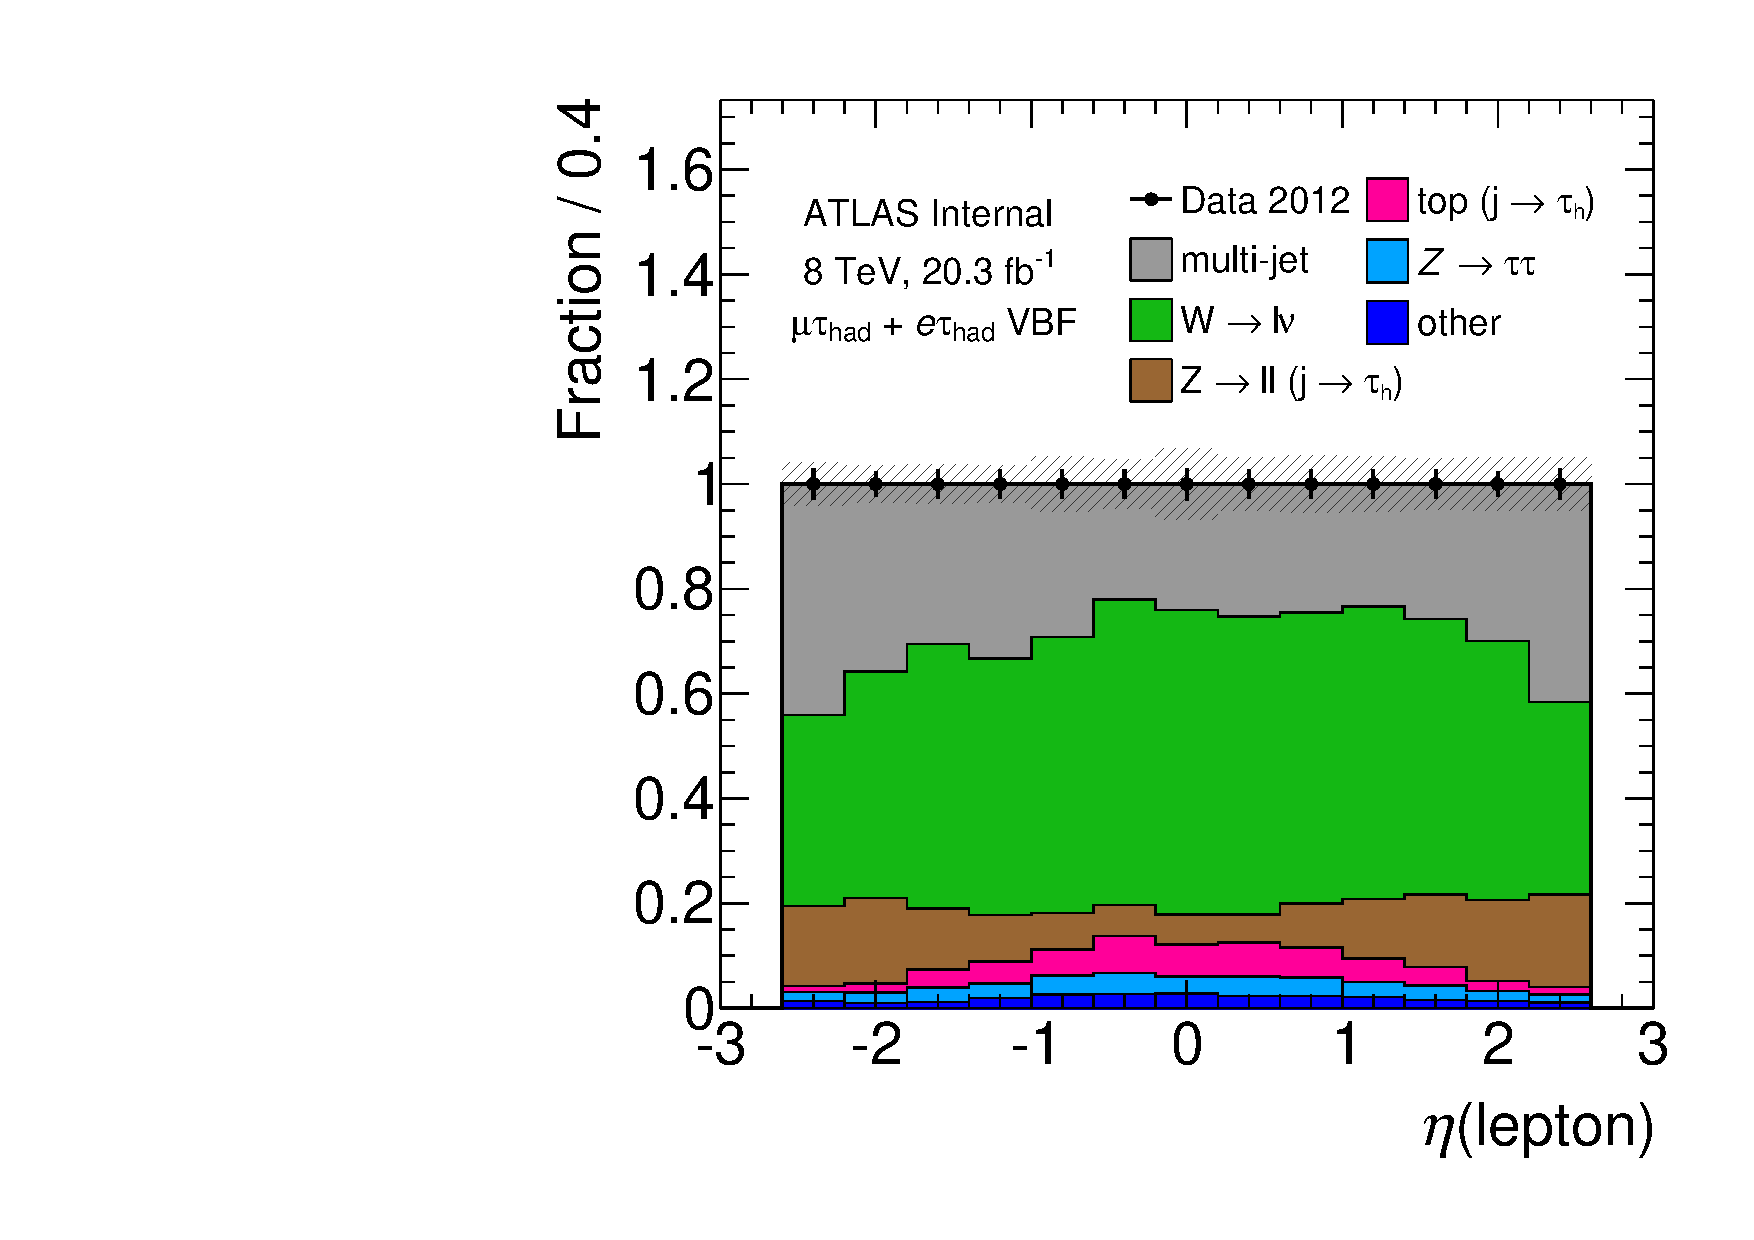
\includegraphics[width=0.32\textwidth]{figures/rx/vbf-mvaSR/lep-eta}
  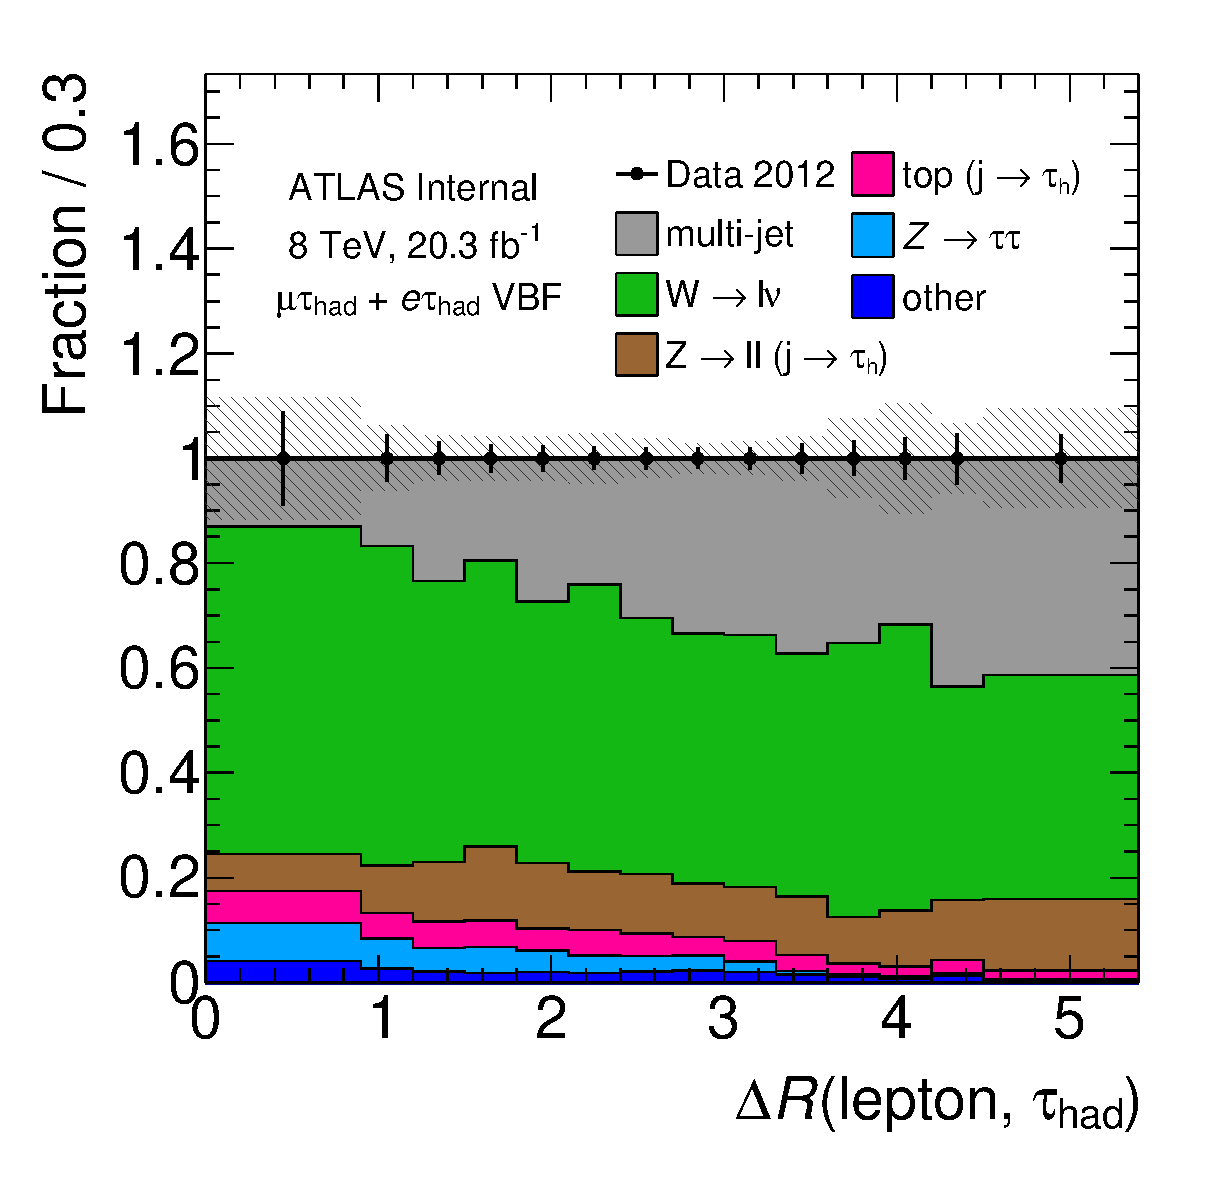
\includegraphics[width=0.32\textwidth]{figures/rx/vbf-mvaSR/taulep-dR}
  % --------------
  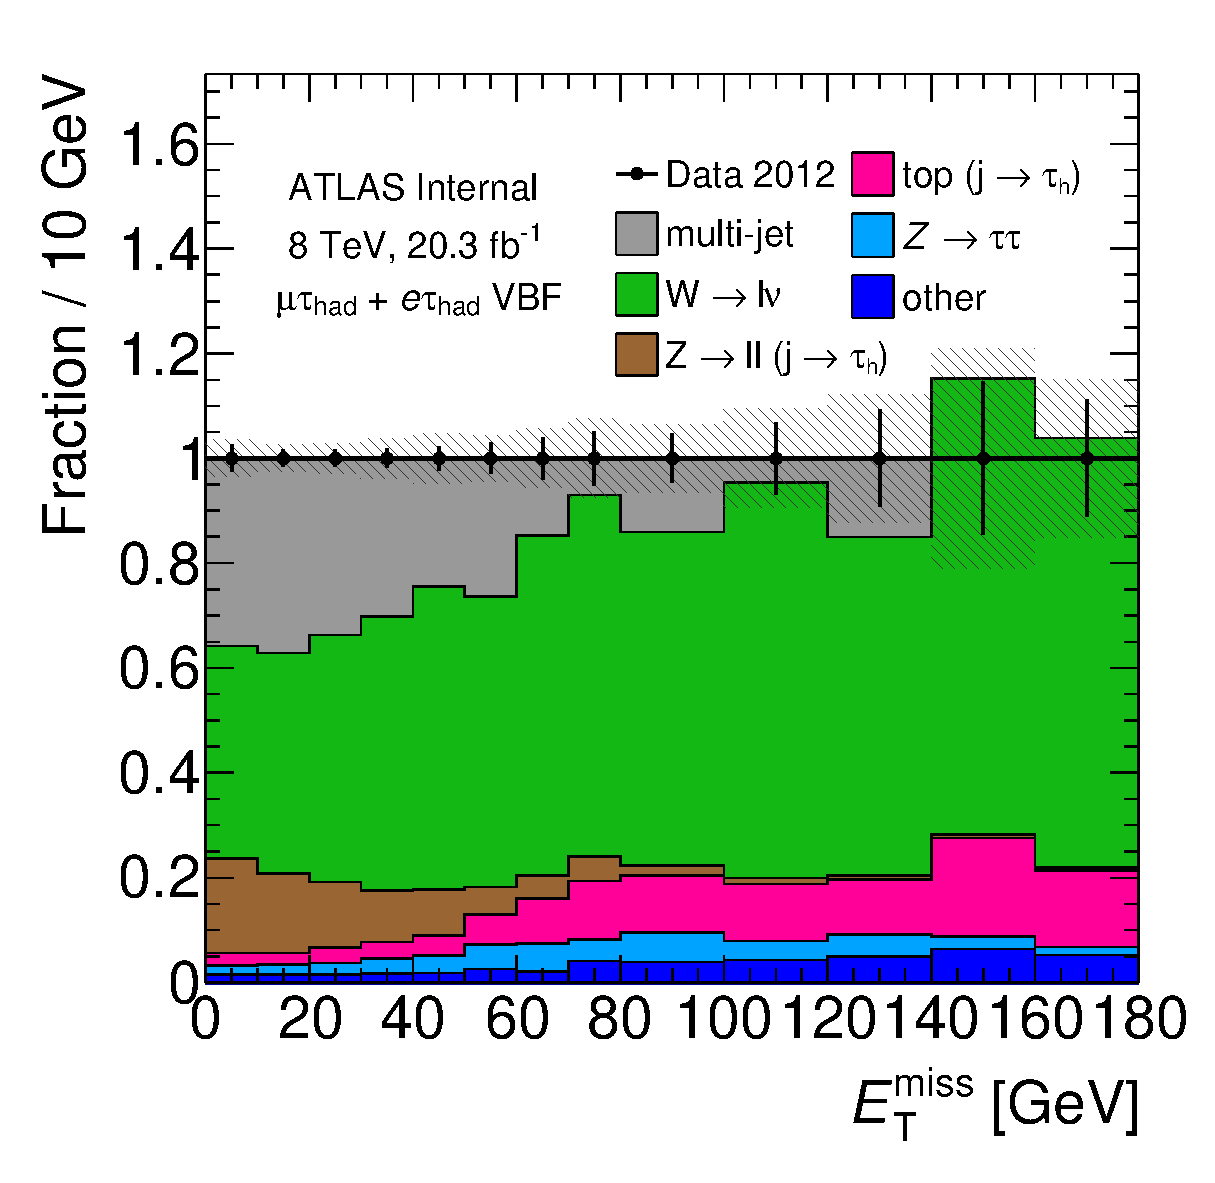
\includegraphics[width=0.32\textwidth]{figures/rx/vbf-mvaSR/met-pt-hi}
  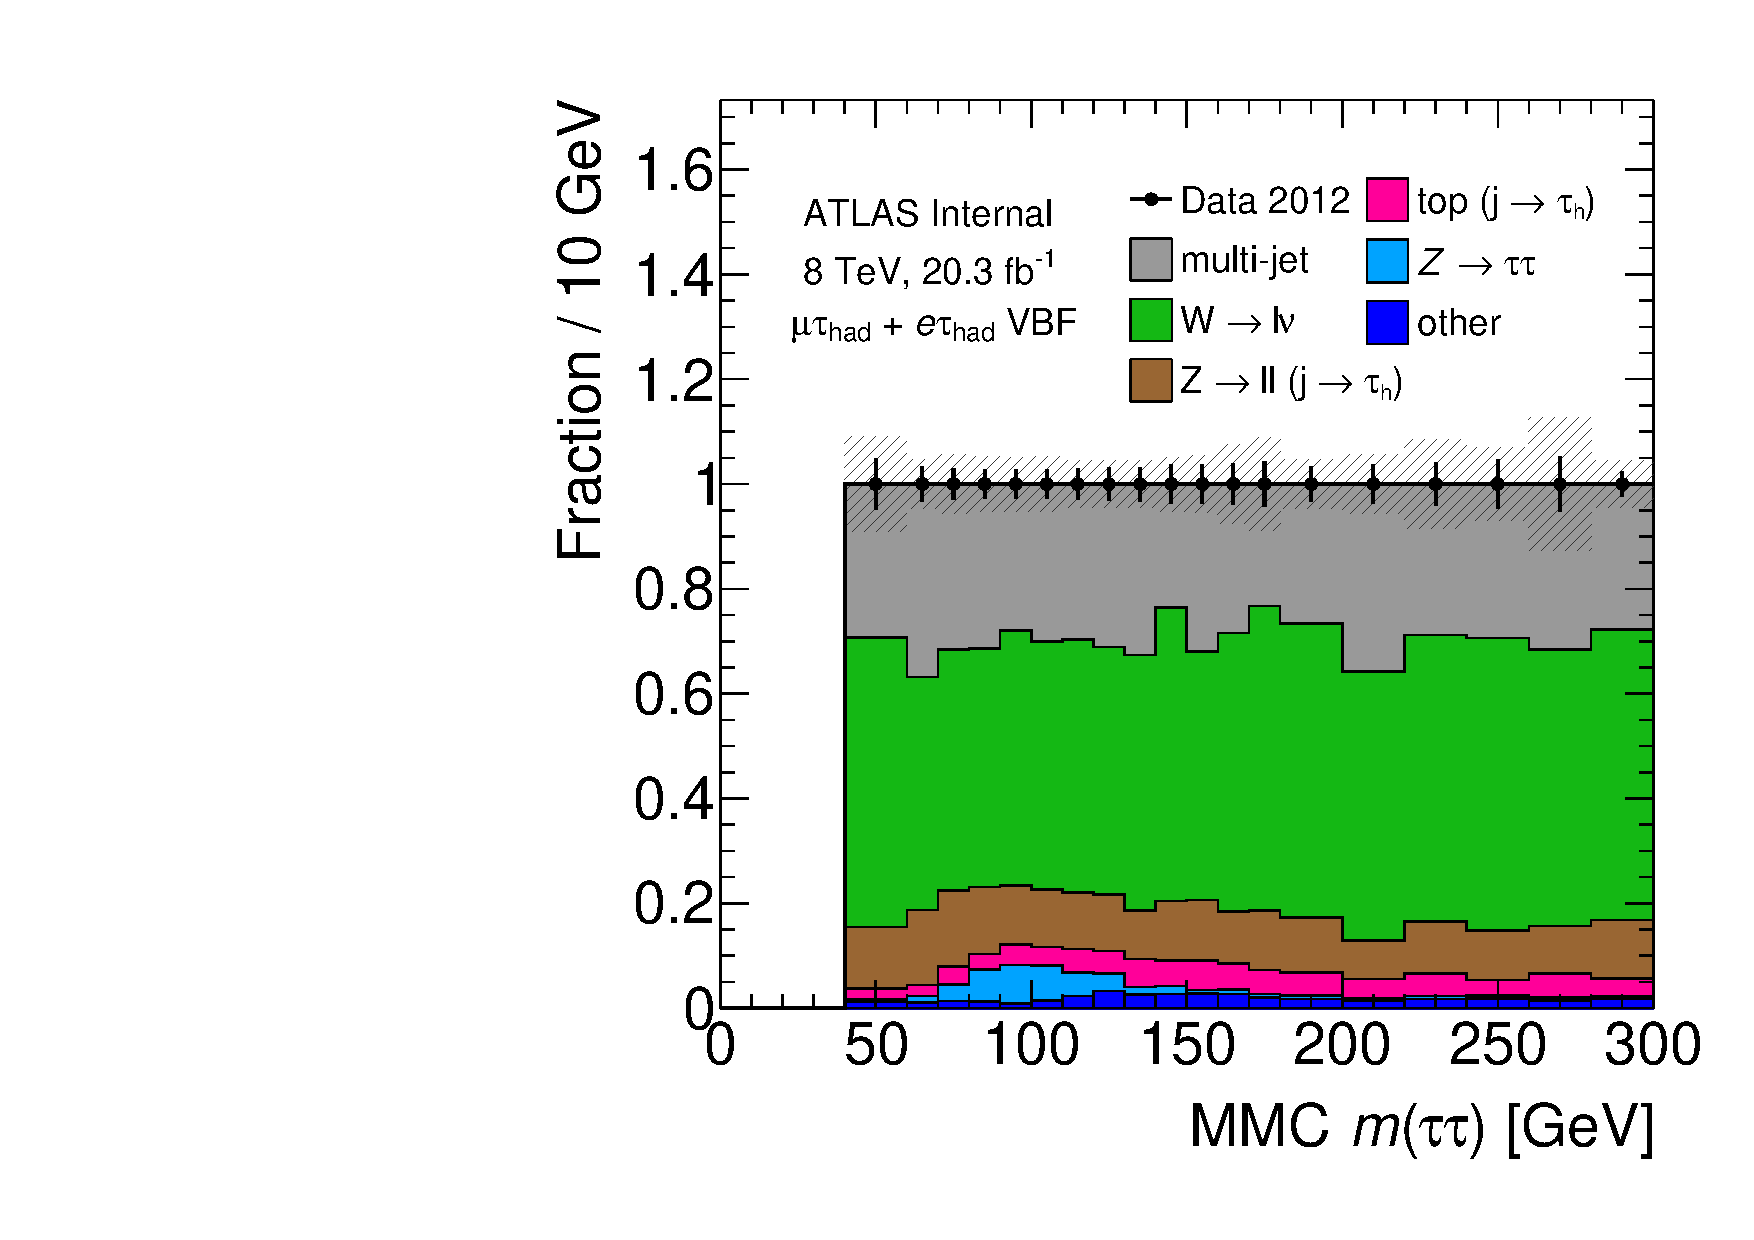
\includegraphics[width=0.32\textwidth]{figures/rx/vbf-mvaSR/mMMC}
  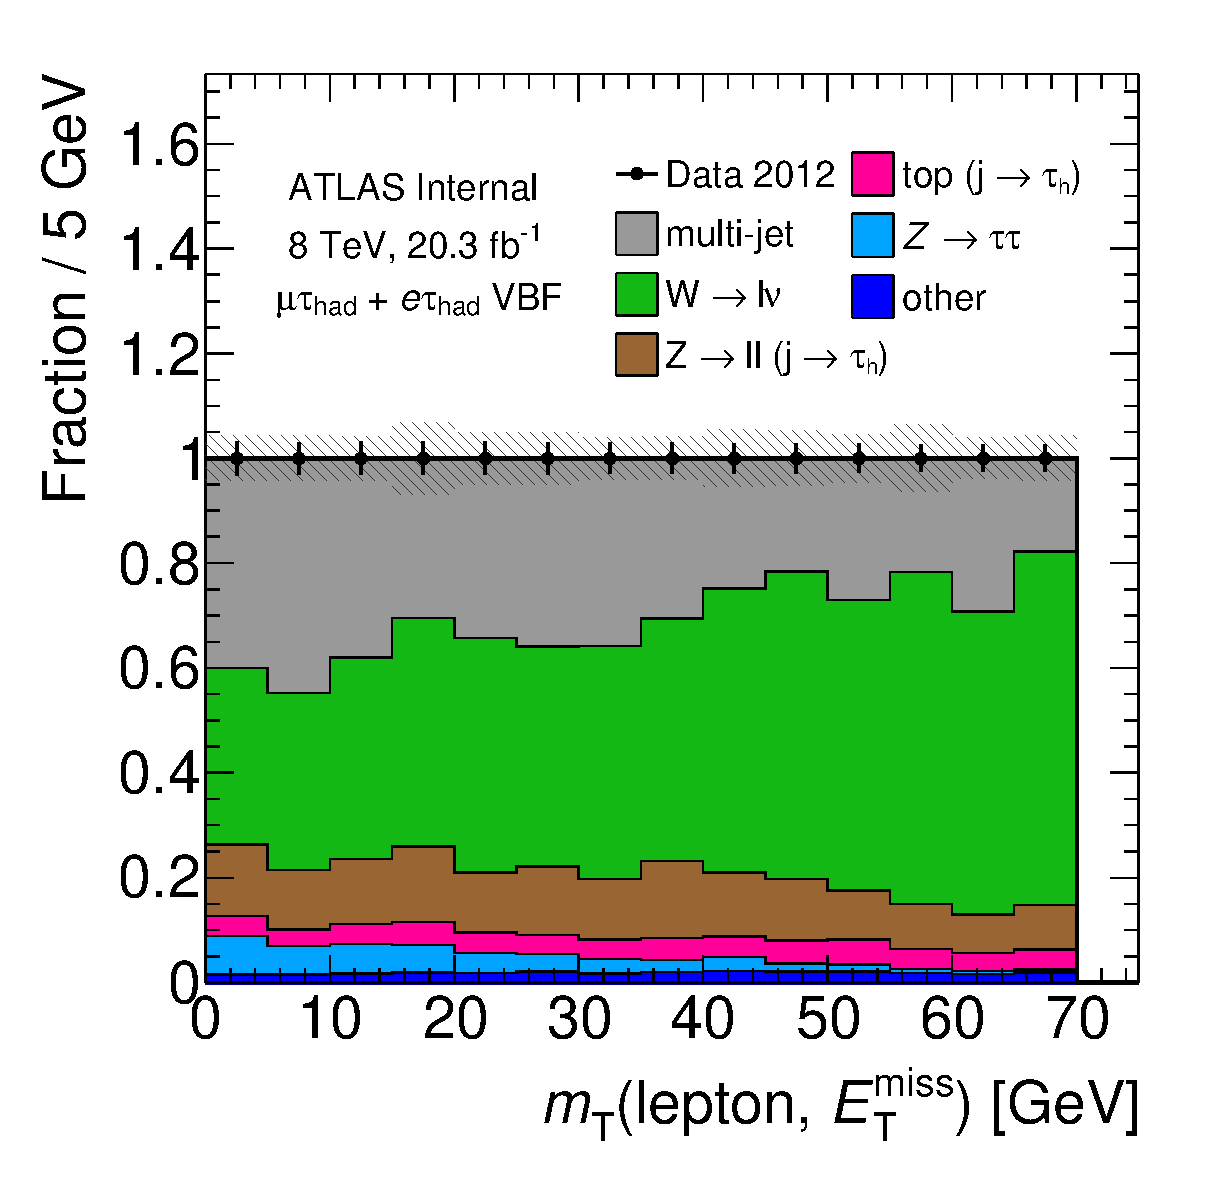
\includegraphics[width=0.32\textwidth]{figures/rx/vbf-mvaSR/mT}
  % --------------
  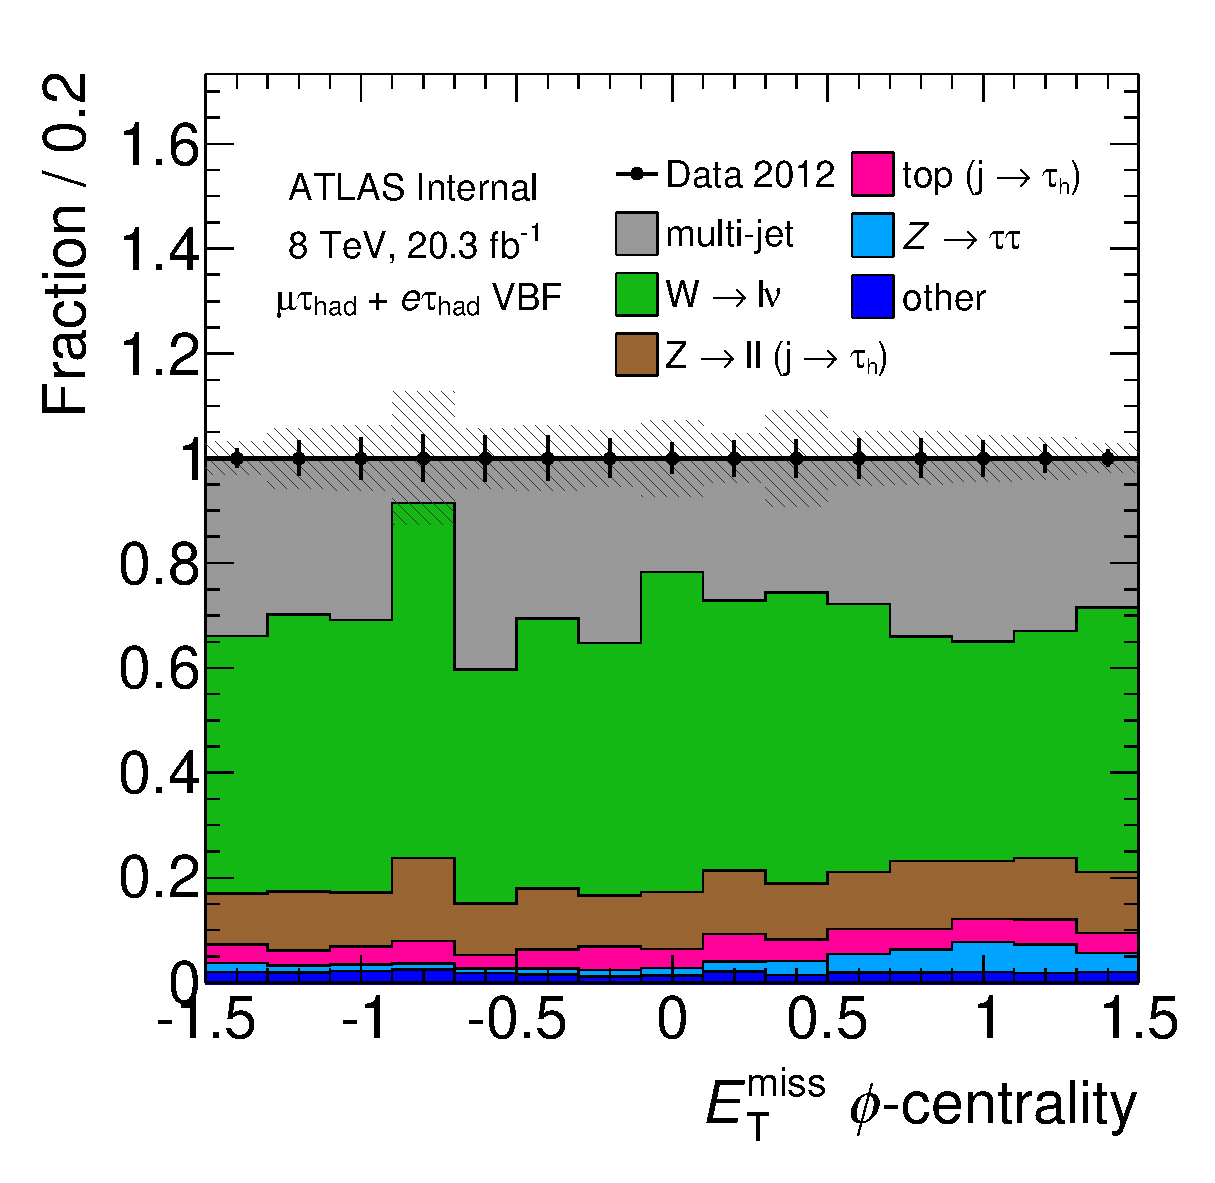
\includegraphics[width=0.32\textwidth]{figures/rx/vbf-mvaSR/met-phi-centrality}
  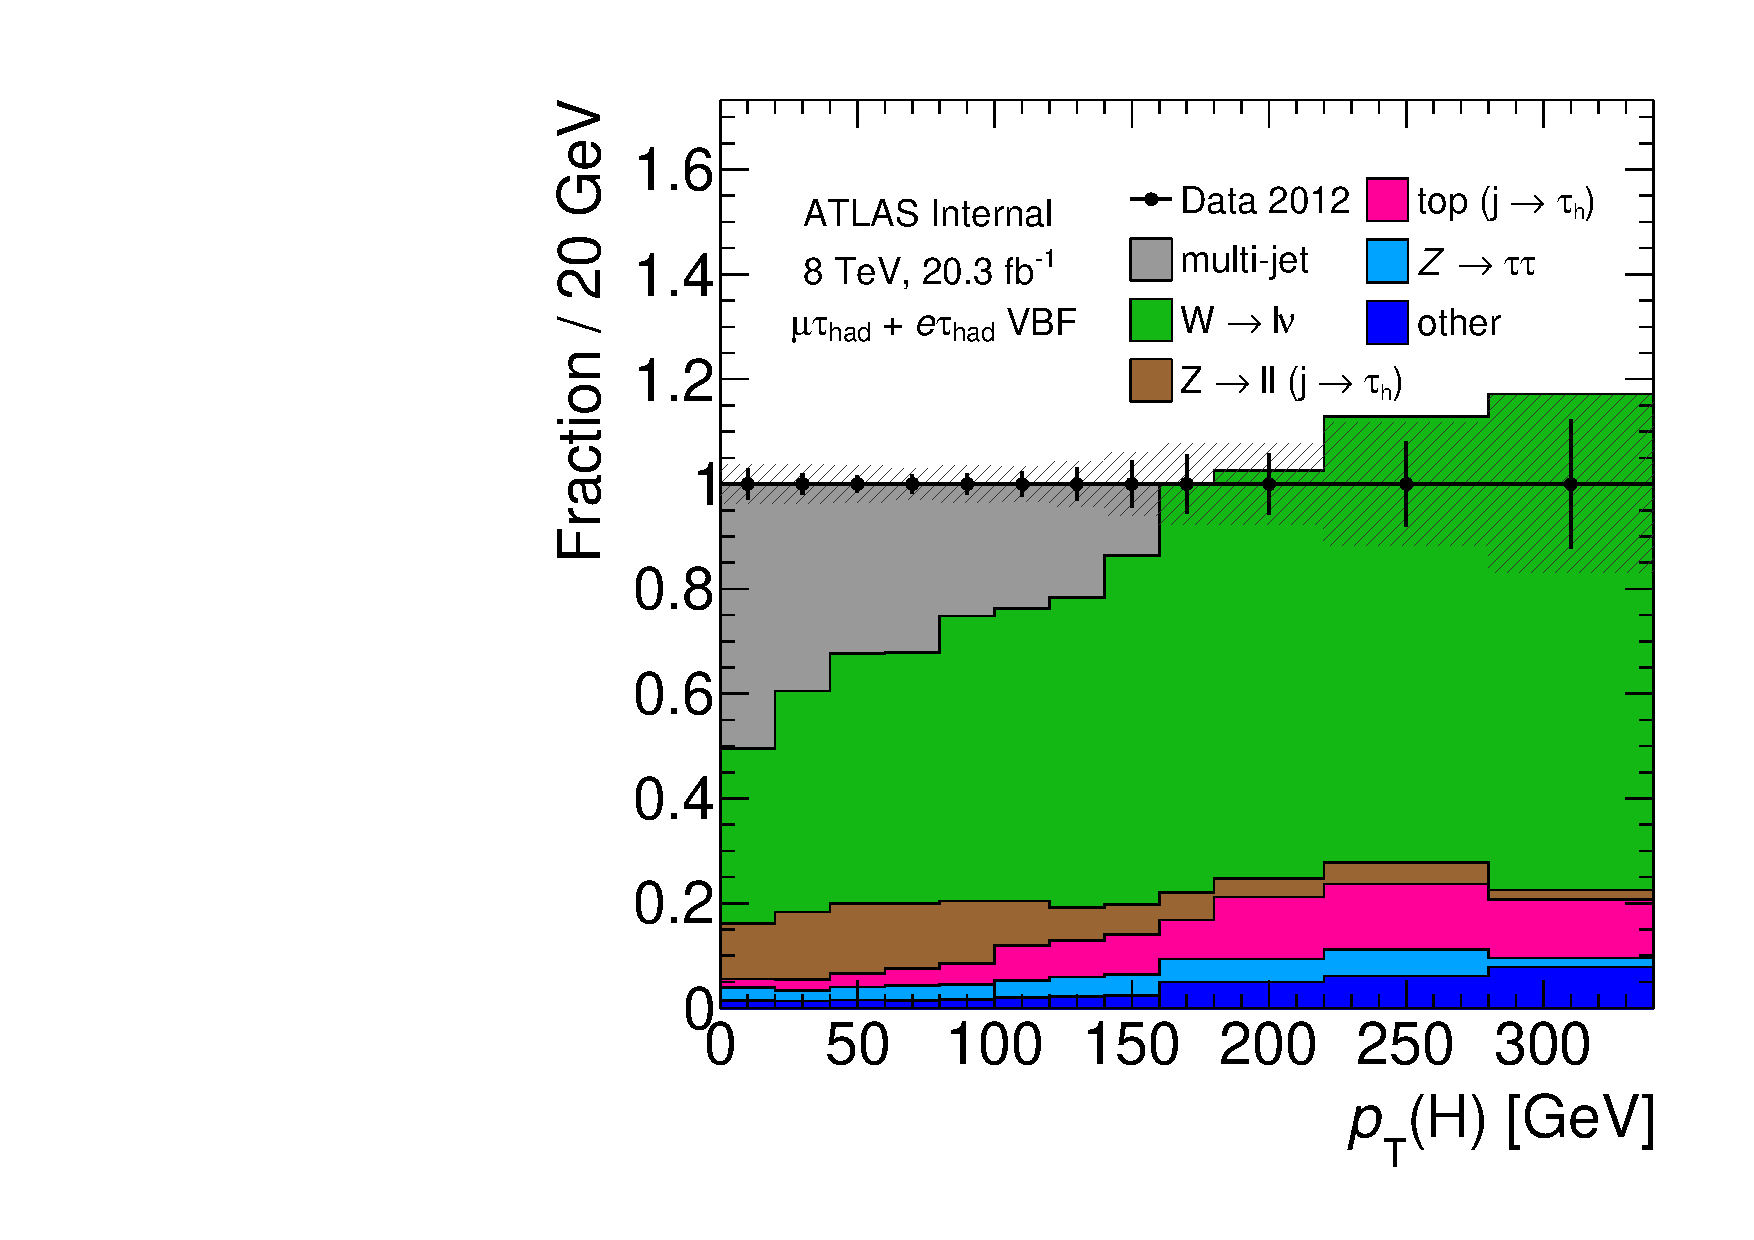
\includegraphics[width=0.32\textwidth]{figures/rx/vbf-mvaSR/H-pt-hi}
  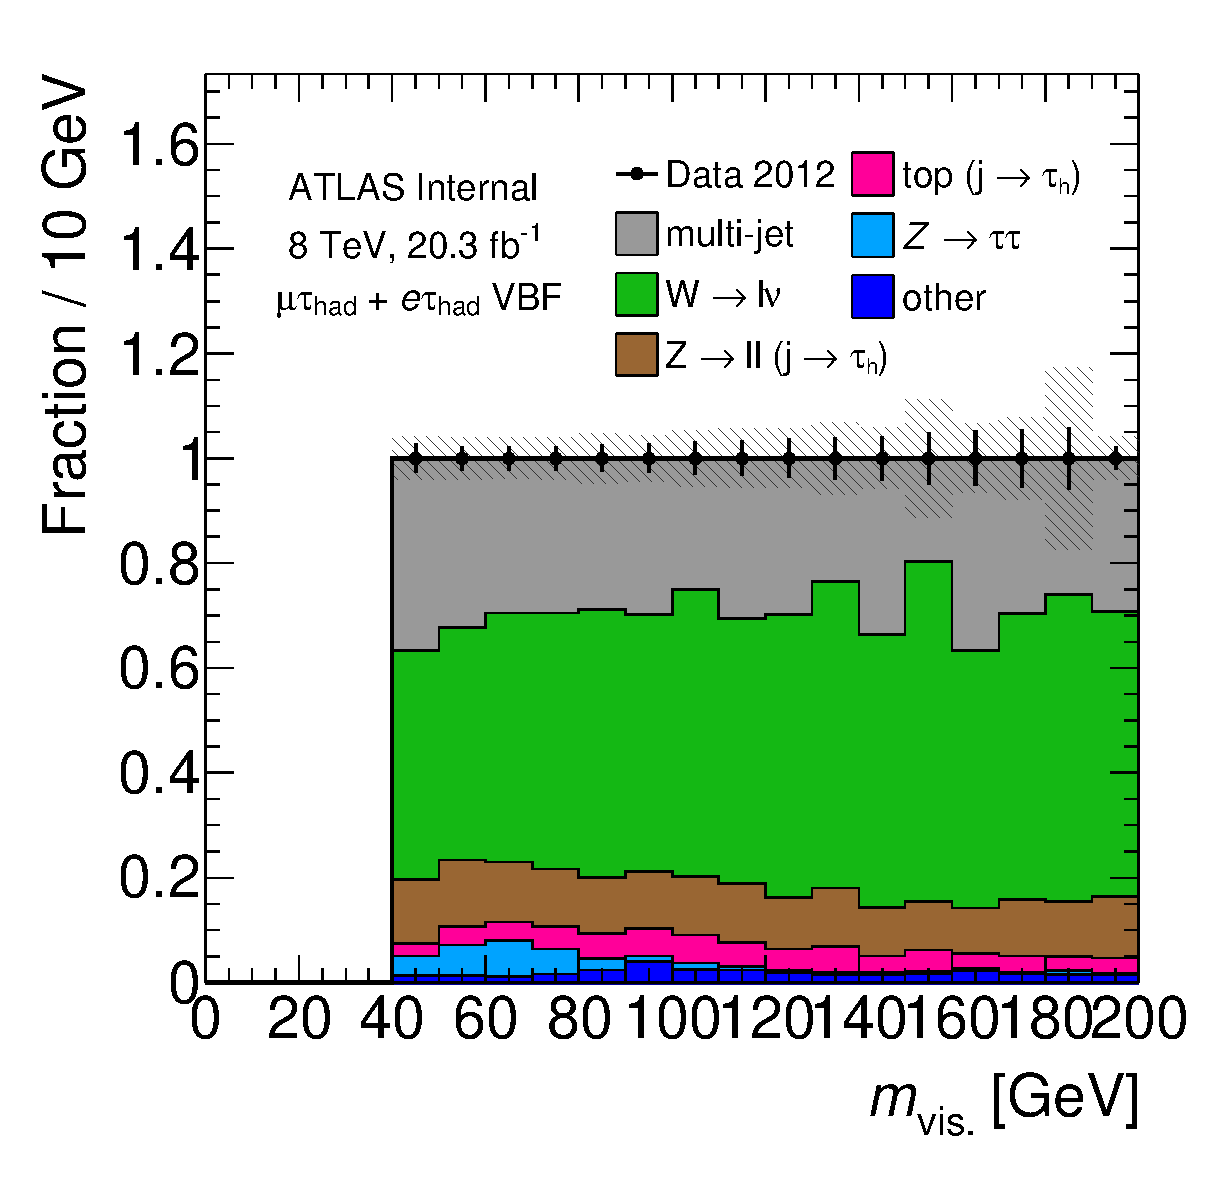
\includegraphics[width=0.32\textwidth]{figures/rx/vbf-mvaSR/mvis}
  \caption{Variables.}
  \label{fig:backgrounds-rx-vbf-taus}
\end{figure}

\clearpage

\begin{figure}[tp]
  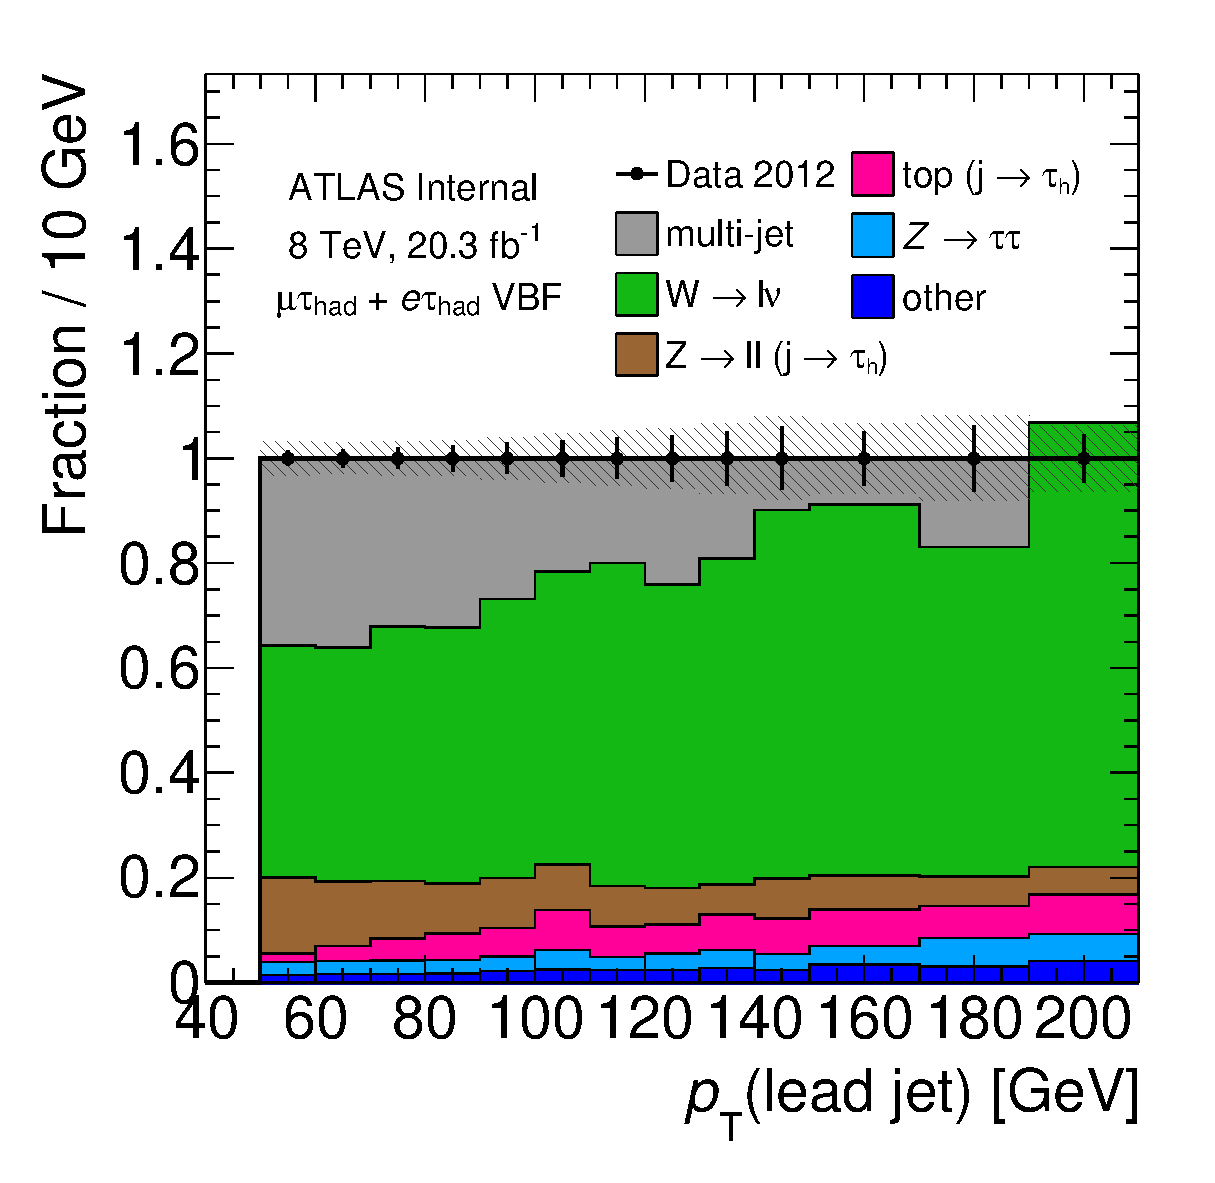
\includegraphics[width=0.32\textwidth]{figures/rx/vbf-mvaSR/jet-1-pt}
  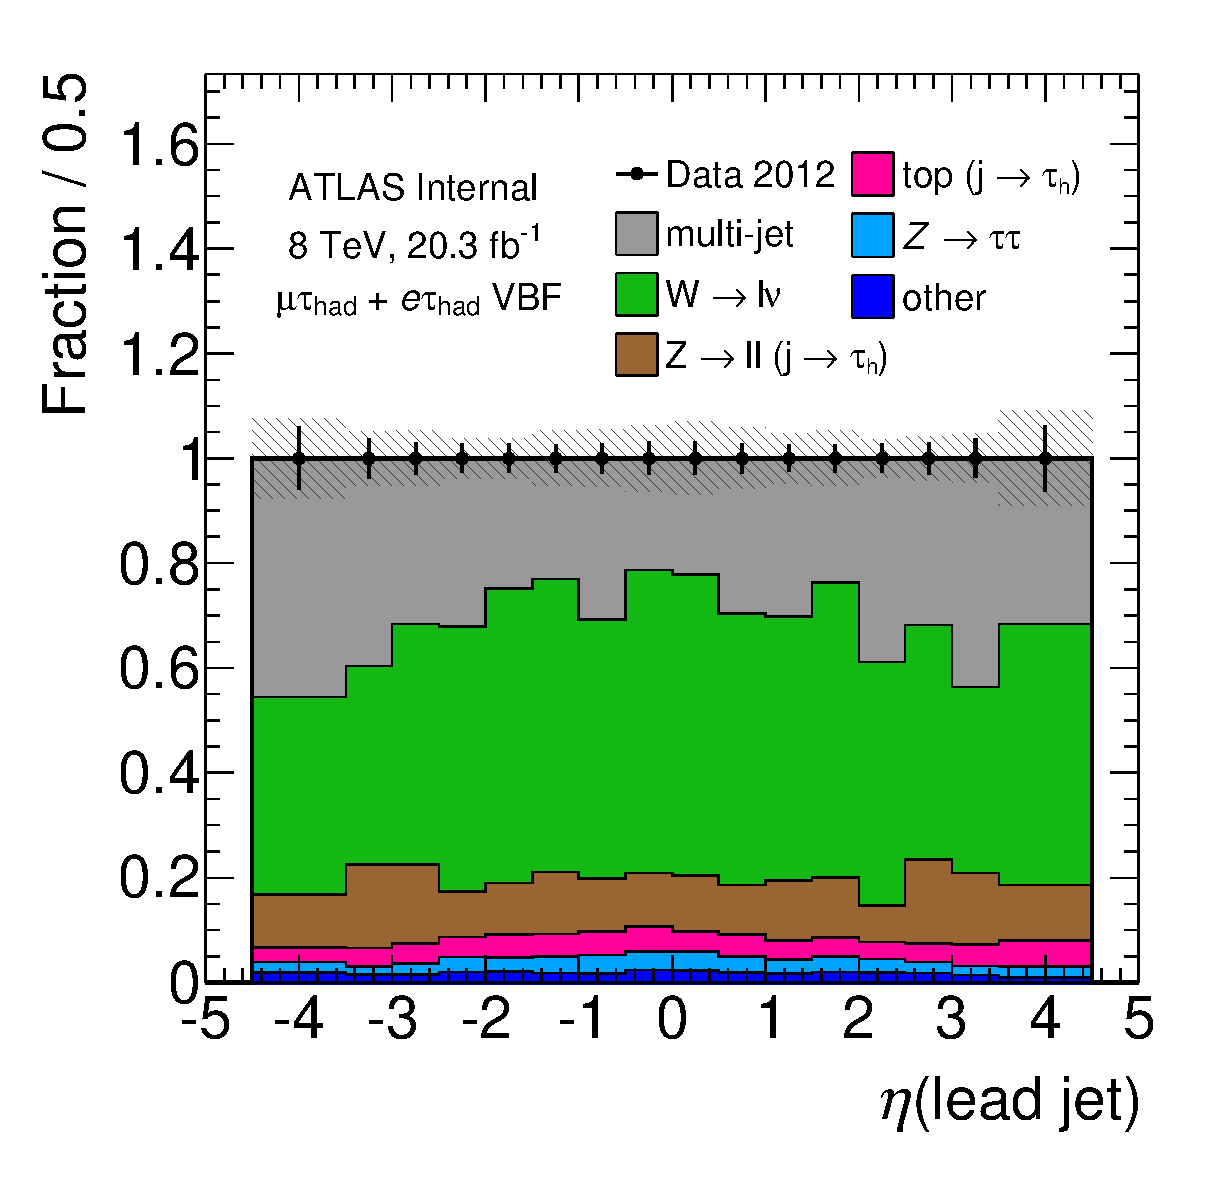
\includegraphics[width=0.32\textwidth]{figures/rx/vbf-mvaSR/jet-1-eta}
  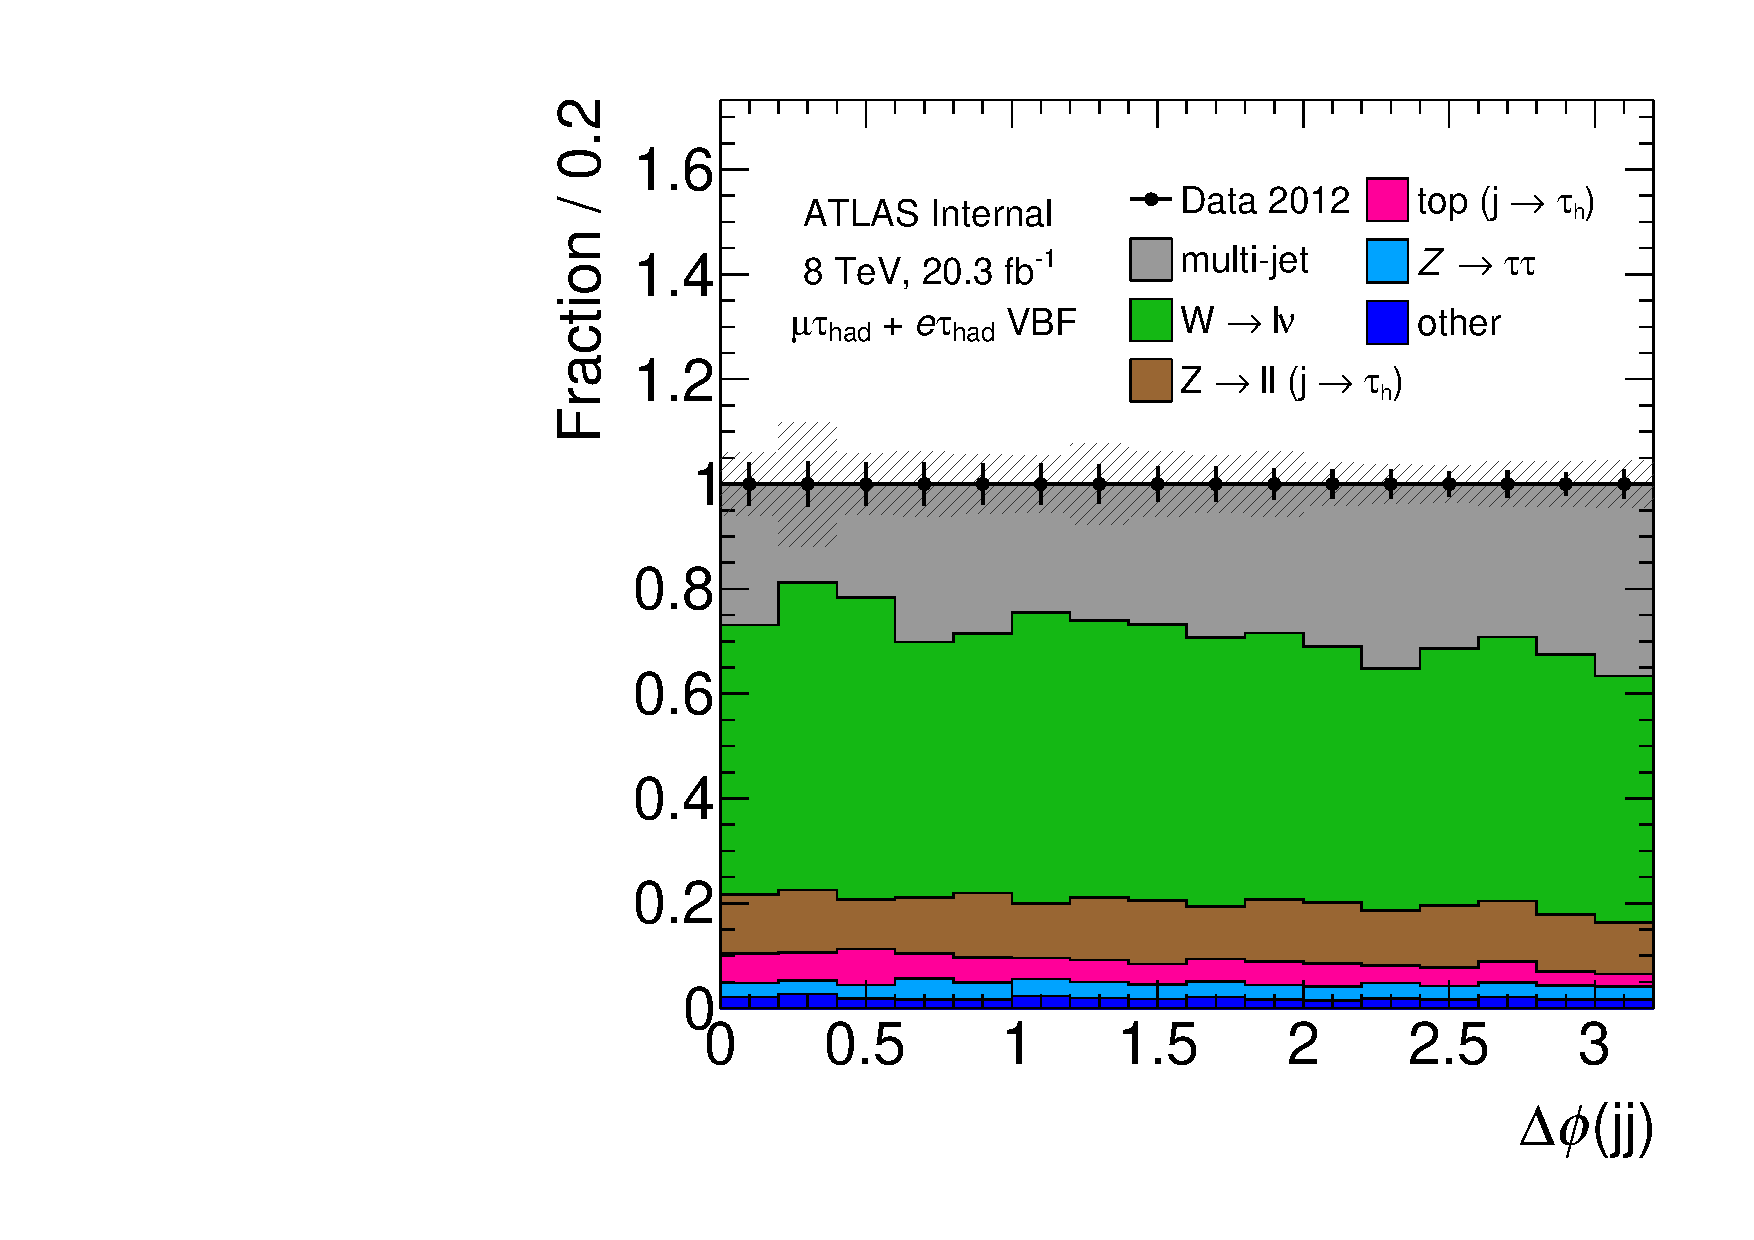
\includegraphics[width=0.32\textwidth]{figures/rx/vbf-mvaSR/jets-dphi}
  % --------------
  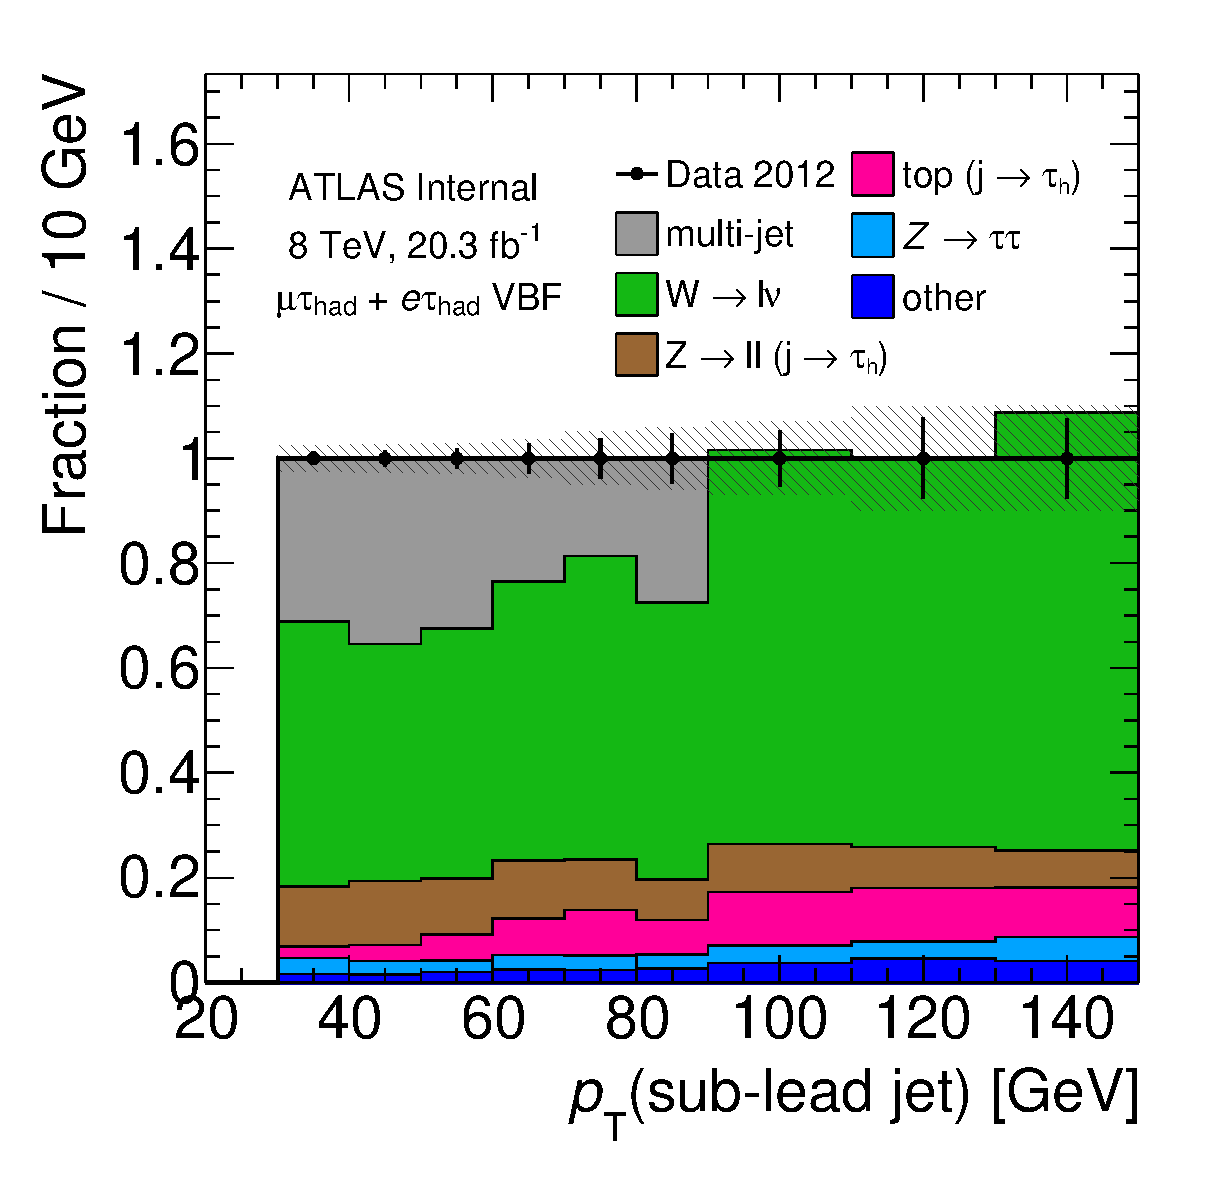
\includegraphics[width=0.32\textwidth]{figures/rx/vbf-mvaSR/jet-2-pt}
  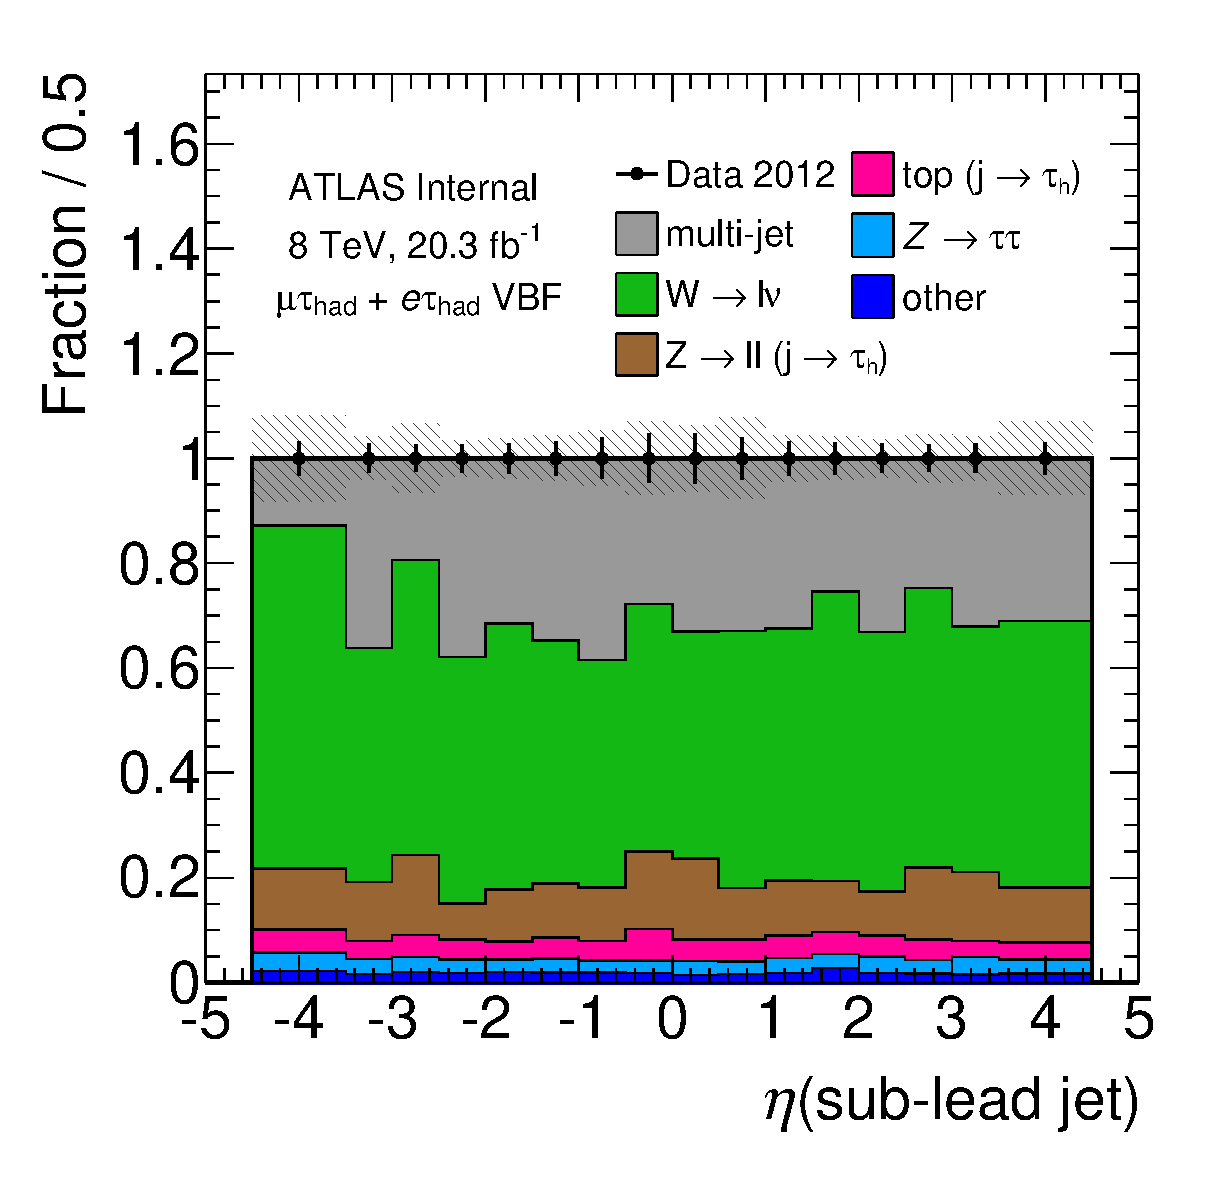
\includegraphics[width=0.32\textwidth]{figures/rx/vbf-mvaSR/jet-2-eta}
  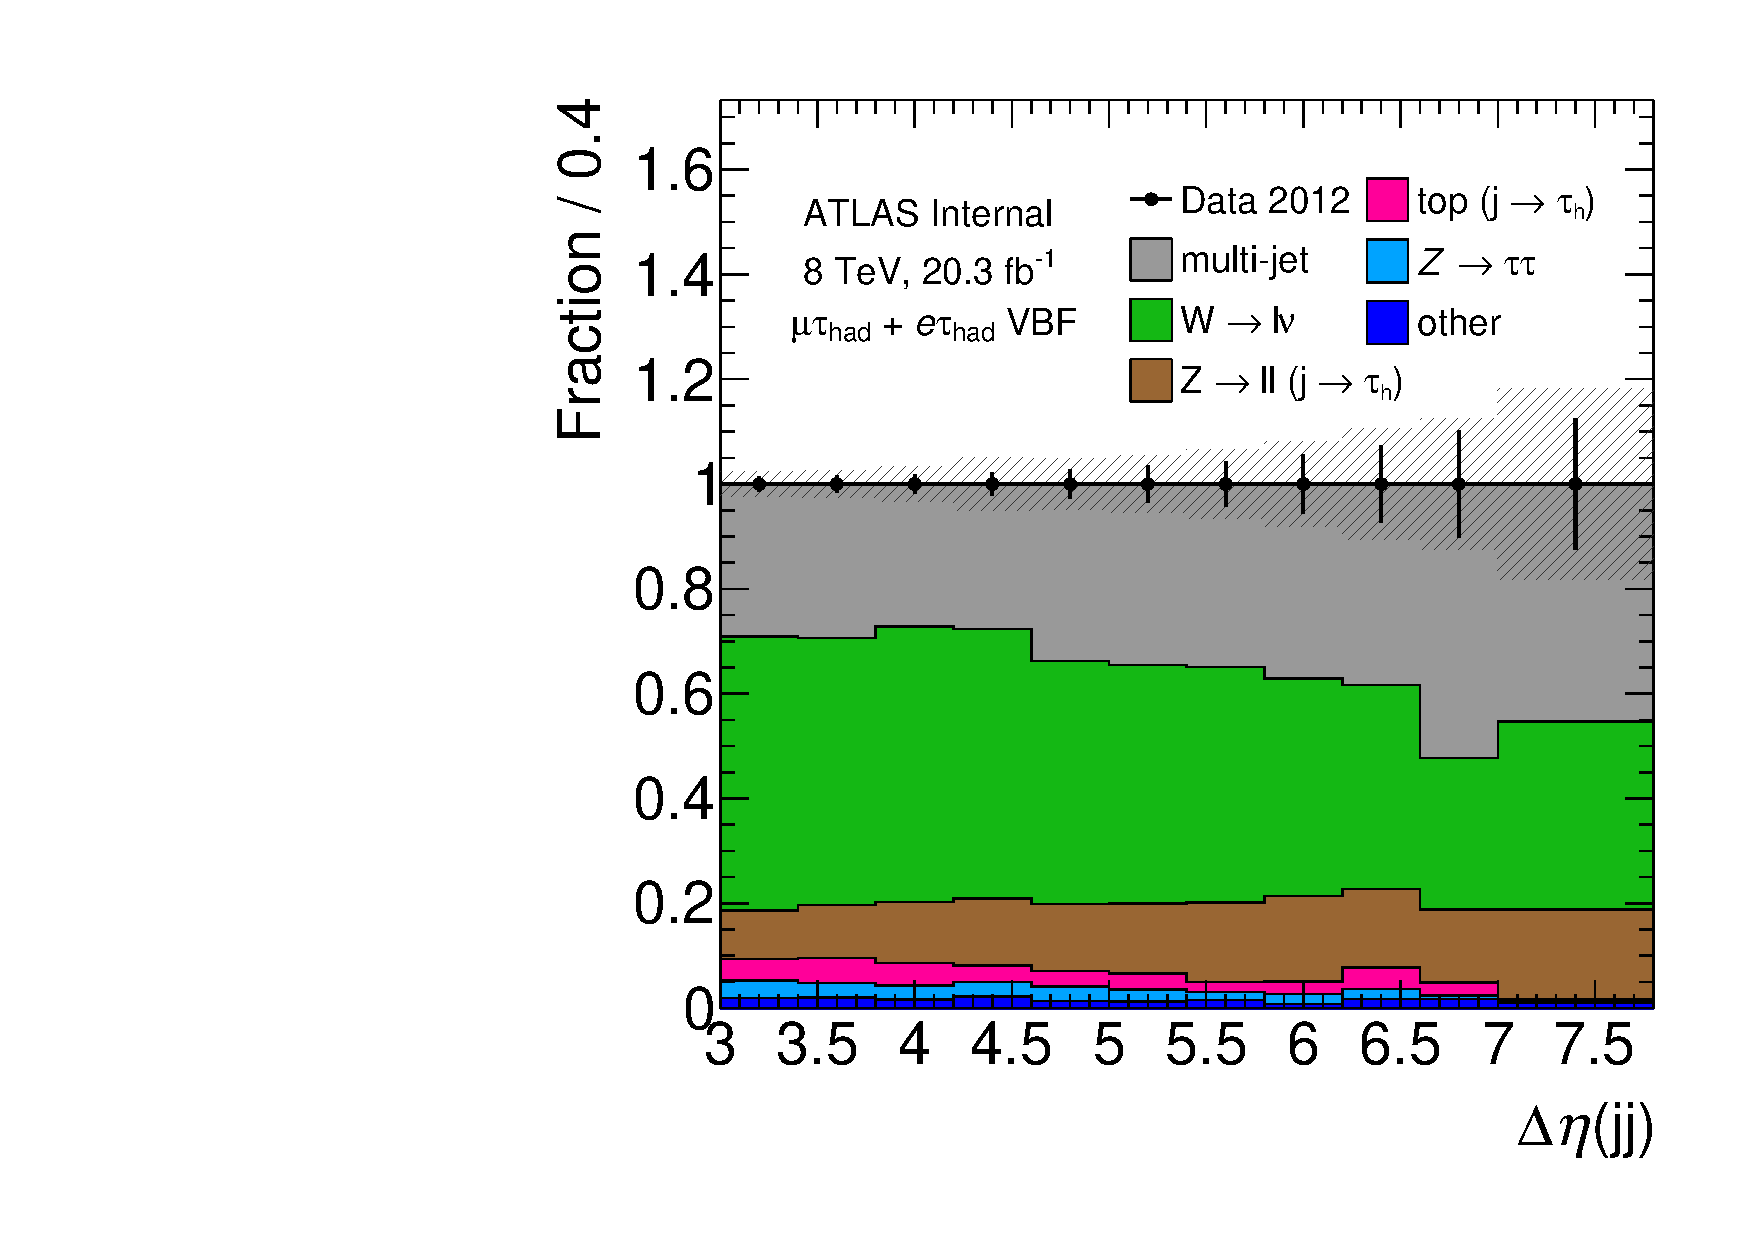
\includegraphics[width=0.32\textwidth]{figures/rx/vbf-mvaSR/jets-deta}
  % --------------
  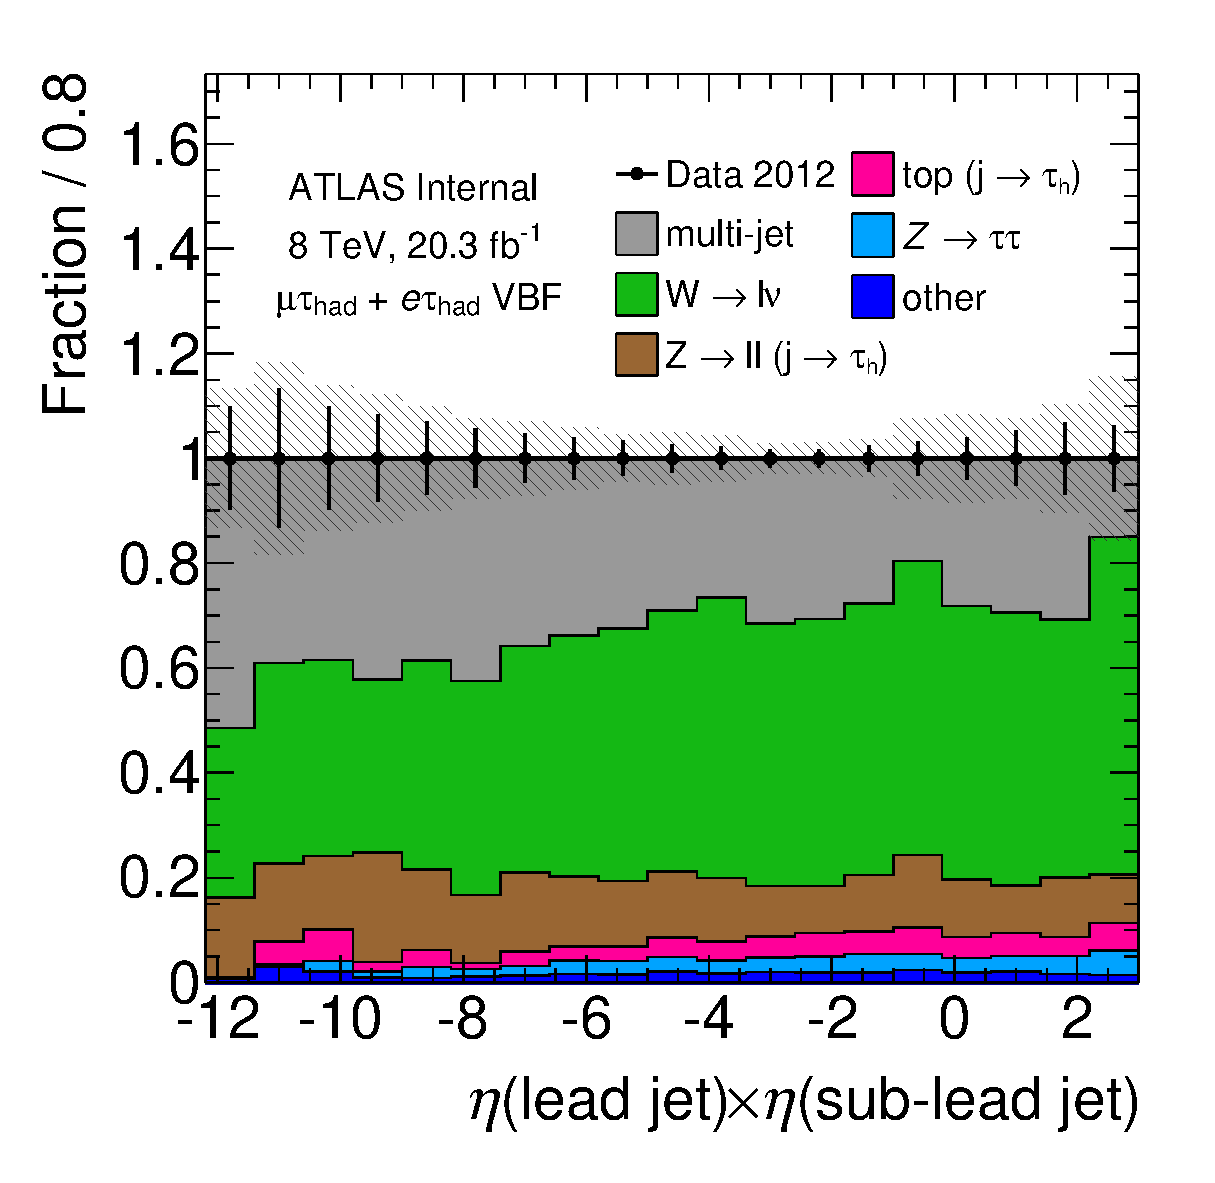
\includegraphics[width=0.32\textwidth]{figures/rx/vbf-mvaSR/jets-etaprod}
  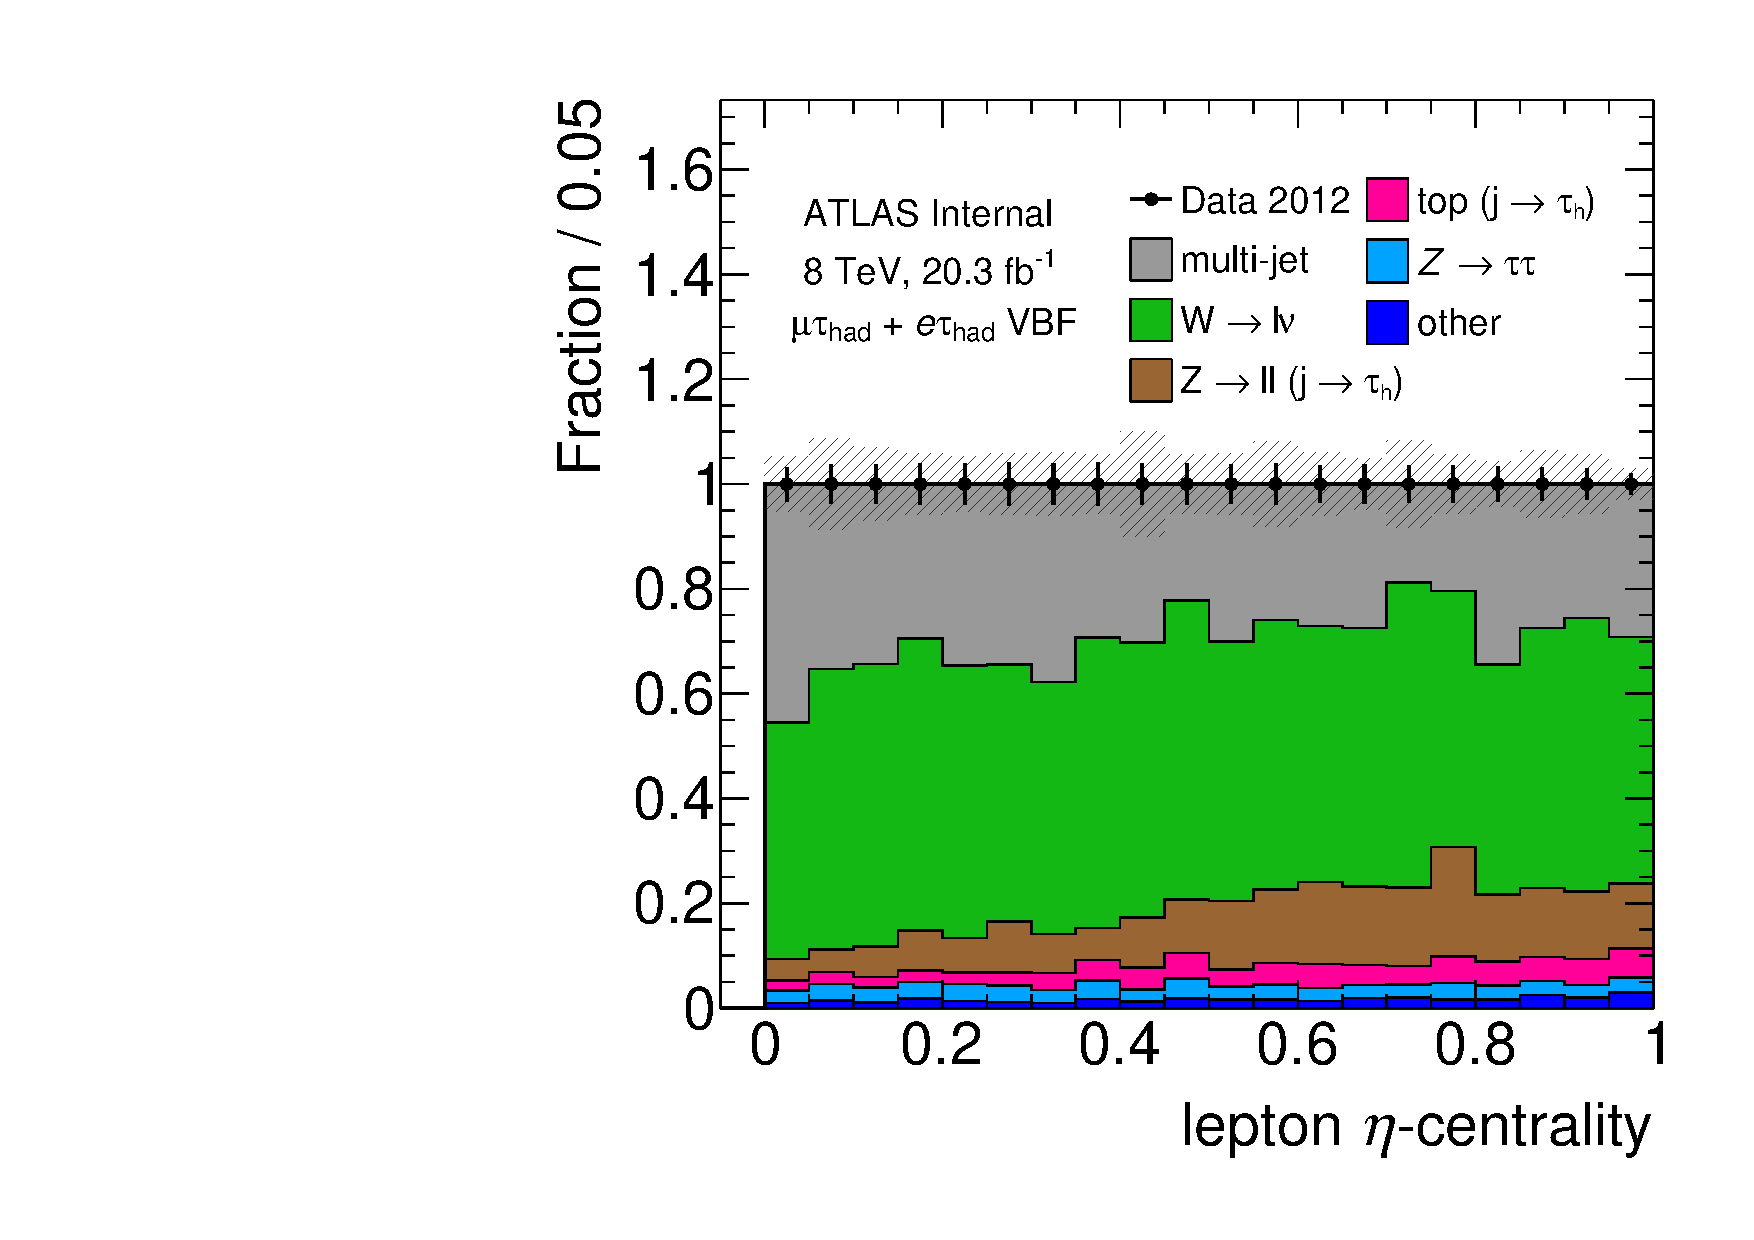
\includegraphics[width=0.32\textwidth]{figures/rx/vbf-mvaSR/lep-eta-centrality}
  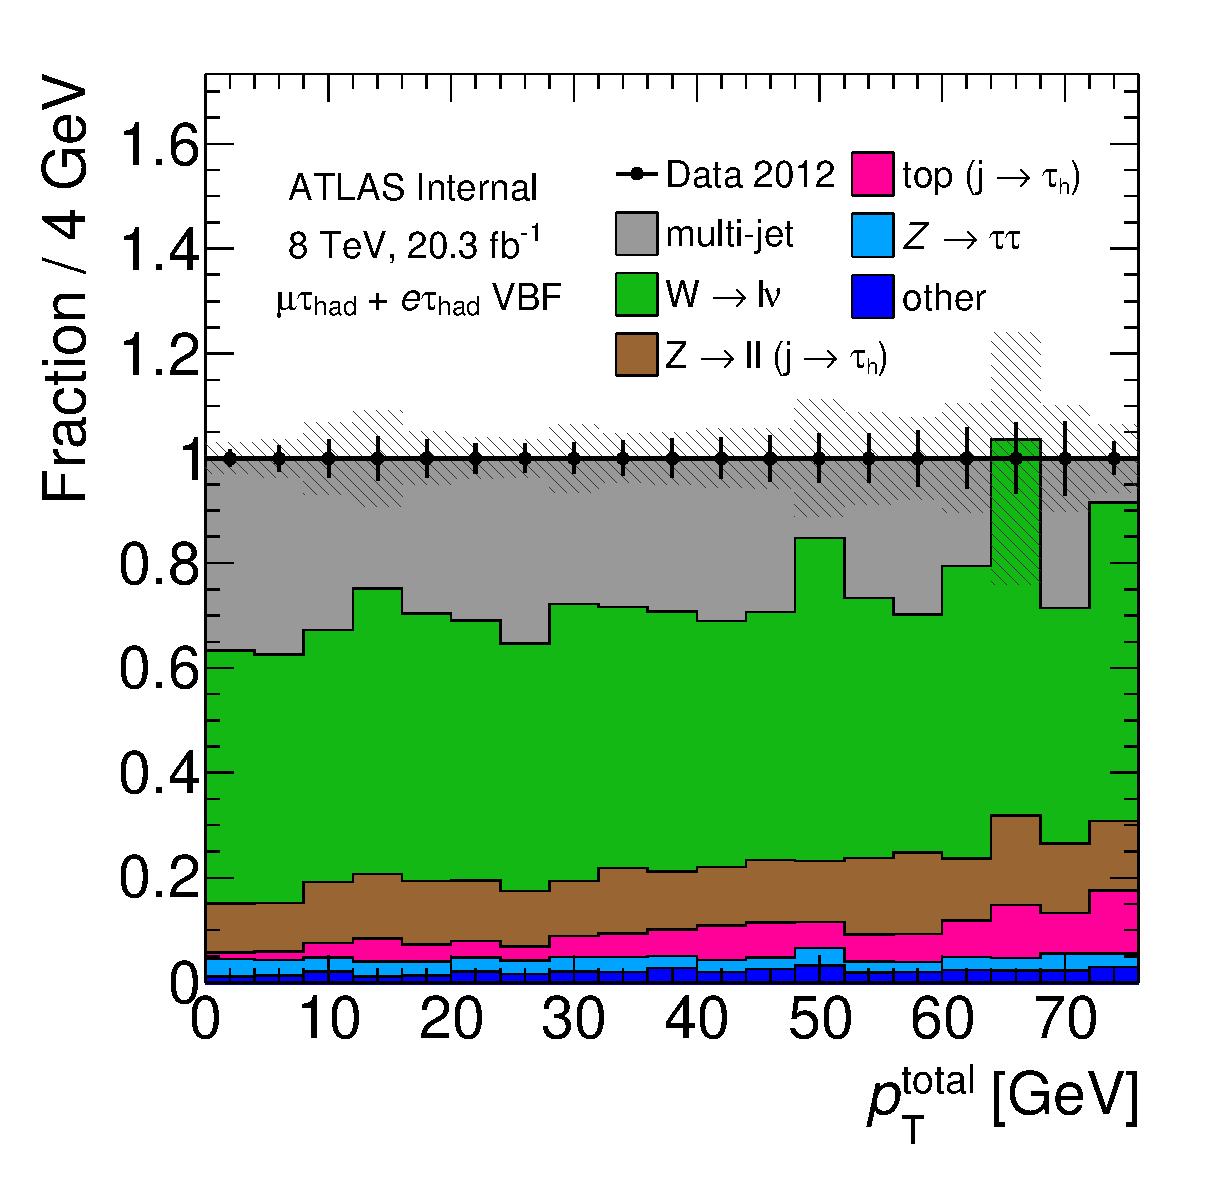
\includegraphics[width=0.32\textwidth]{figures/rx/vbf-mvaSR/system-pt}
  % --------------
  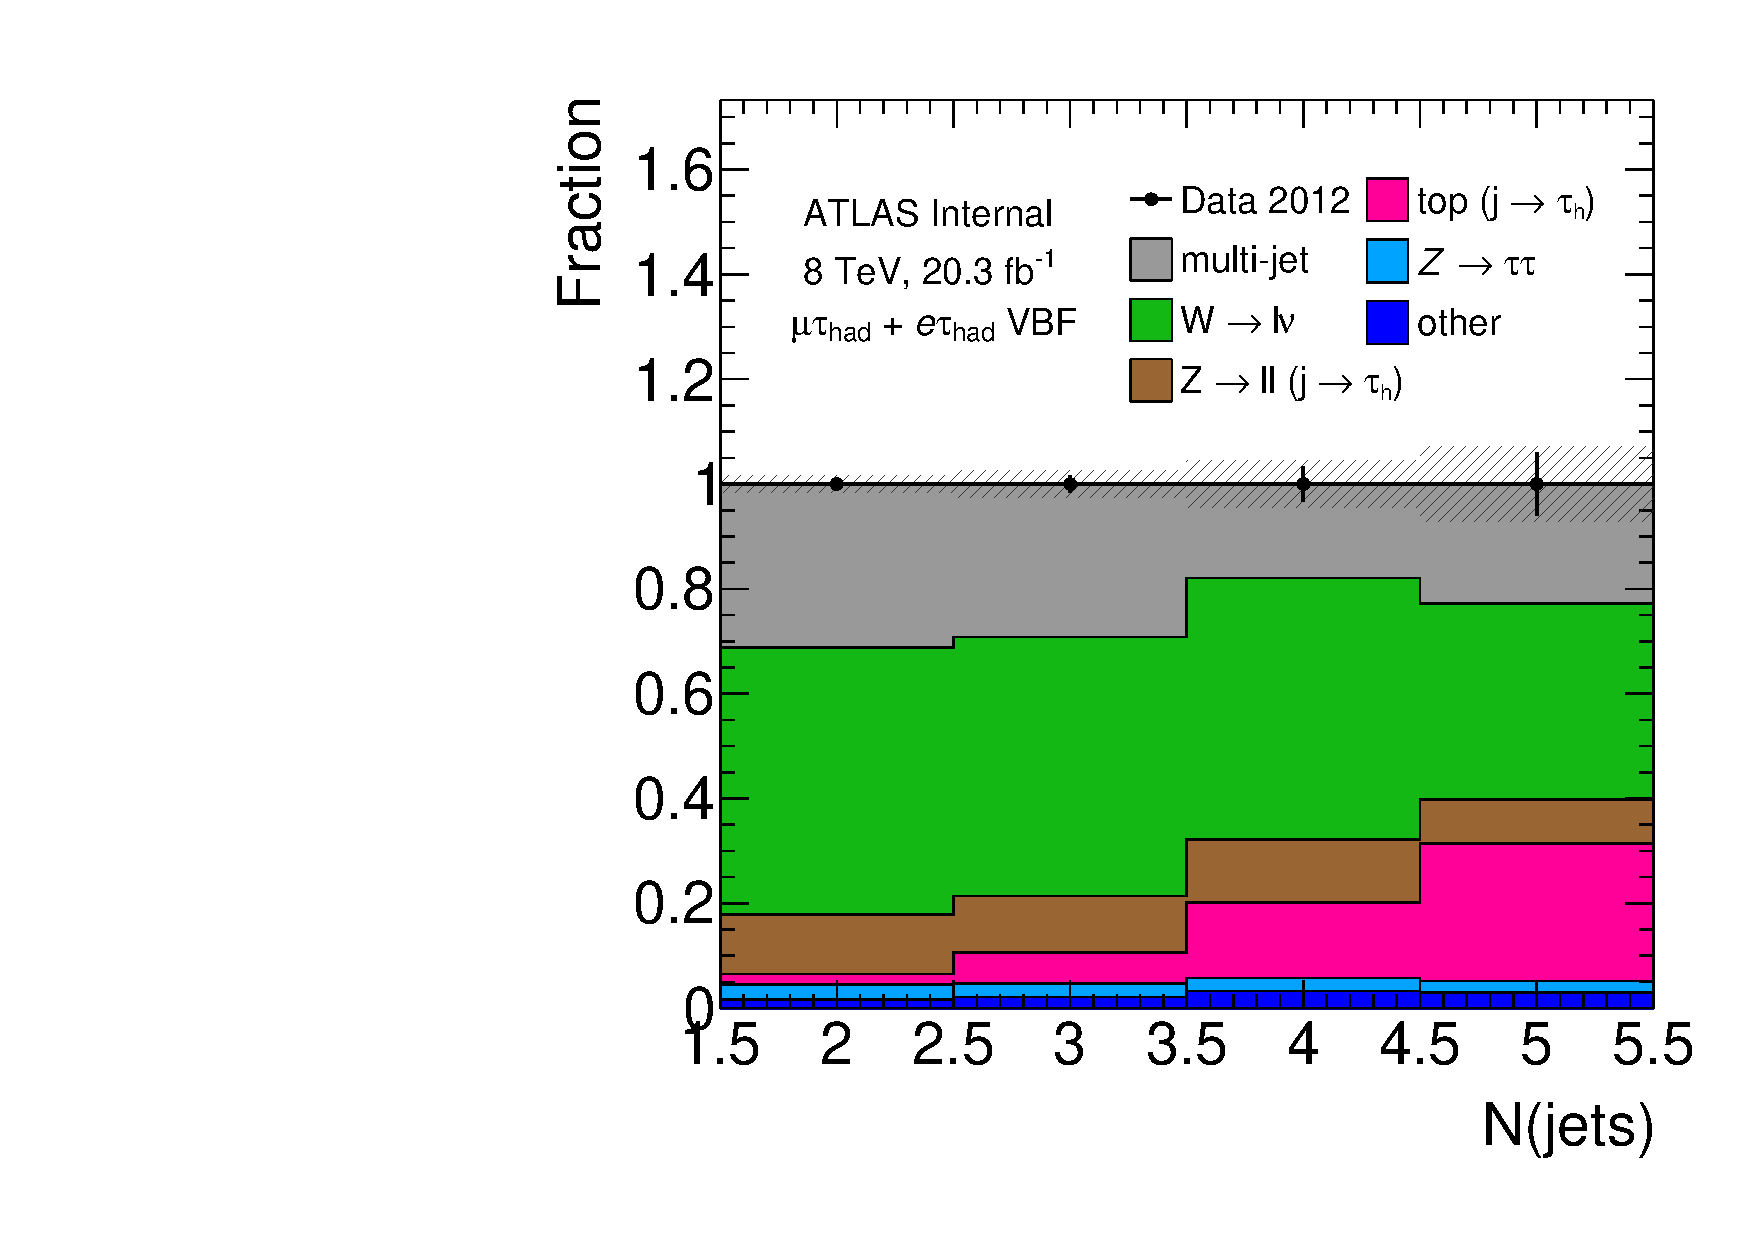
\includegraphics[width=0.32\textwidth]{figures/rx/vbf-mvaSR/n-jets30}
  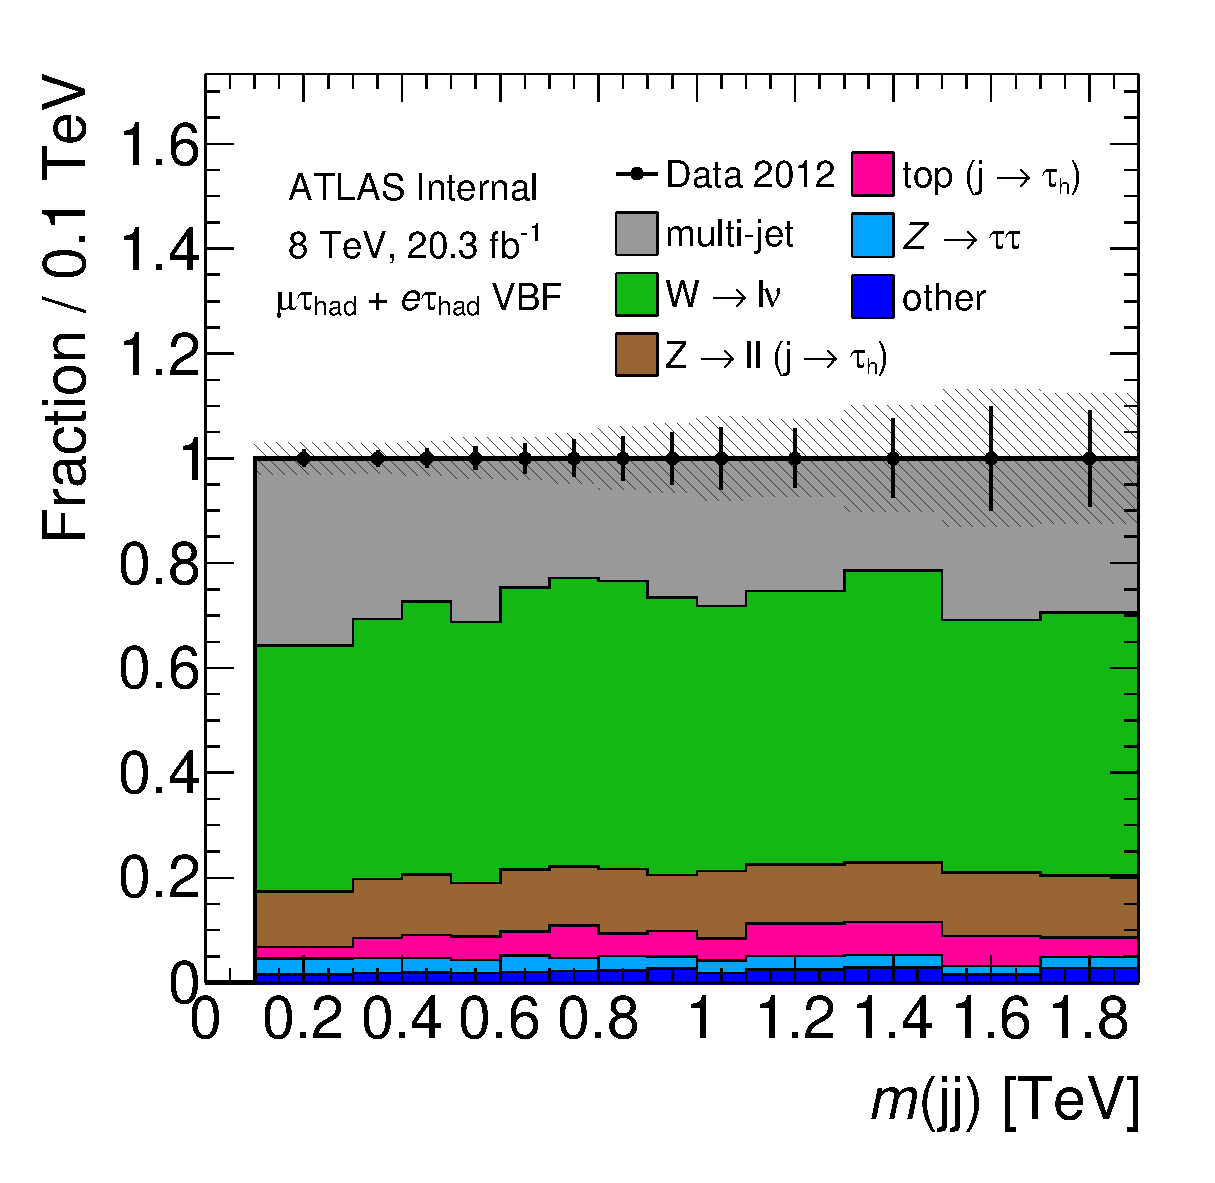
\includegraphics[width=0.32\textwidth]{figures/rx/vbf-mvaSR/dijet-m-veryhigh}
  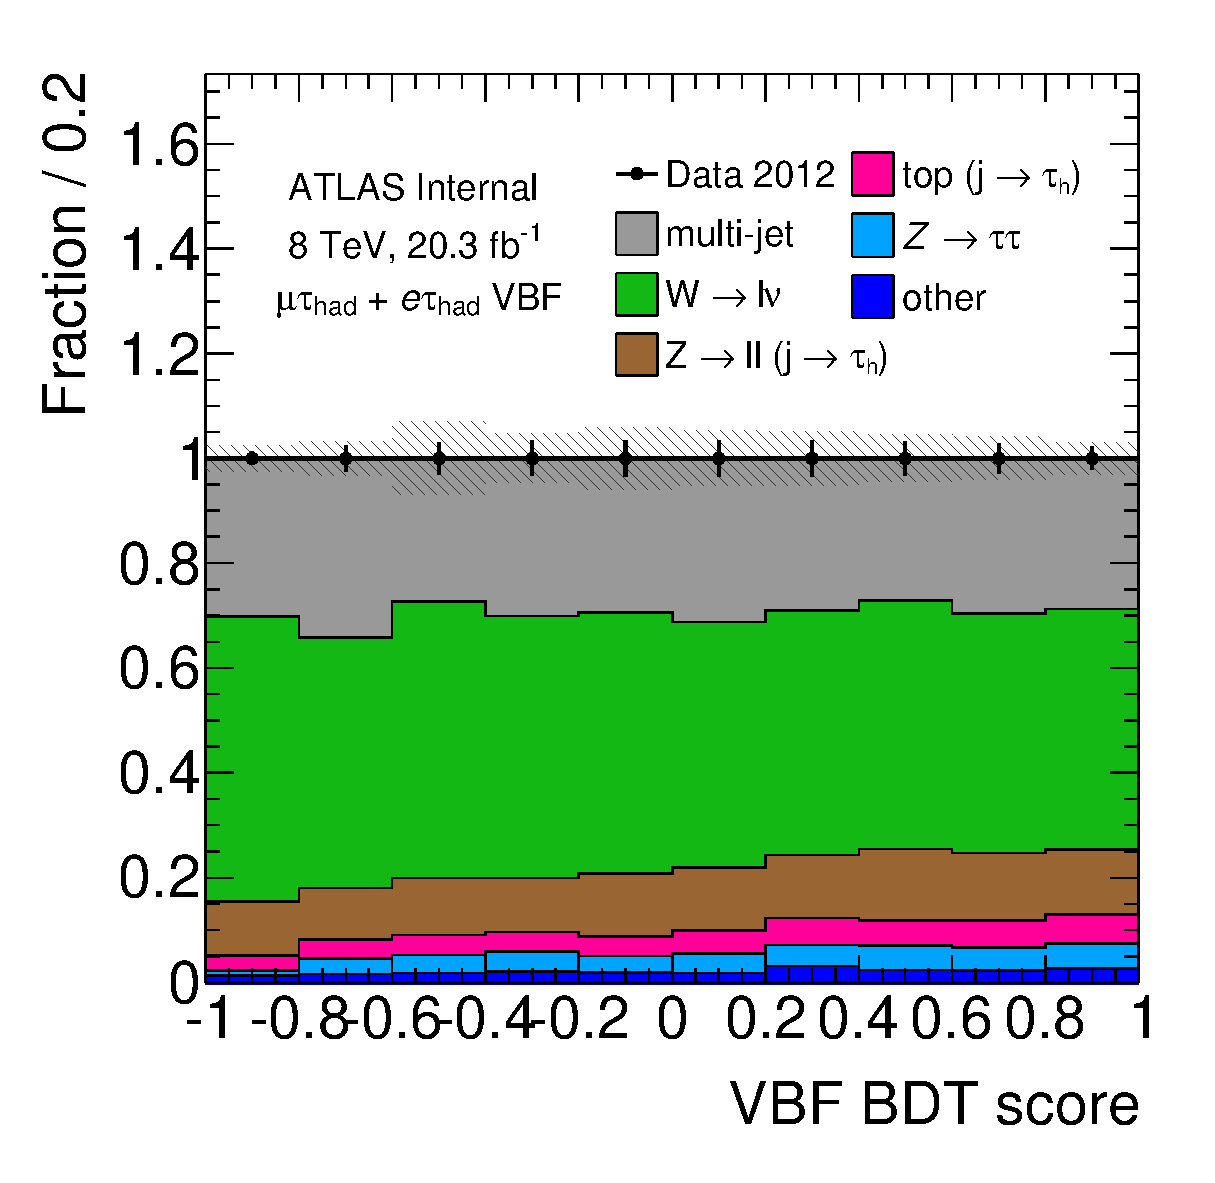
\includegraphics[width=0.32\textwidth]{figures/rx/vbf-mvaSR/BDTEve-VBF}
  \caption{Variables.}
  \label{fig:backgrounds-rx-vbf-jets}
\end{figure}

\clearpage

\begin{figure}[tp]
  \centering
  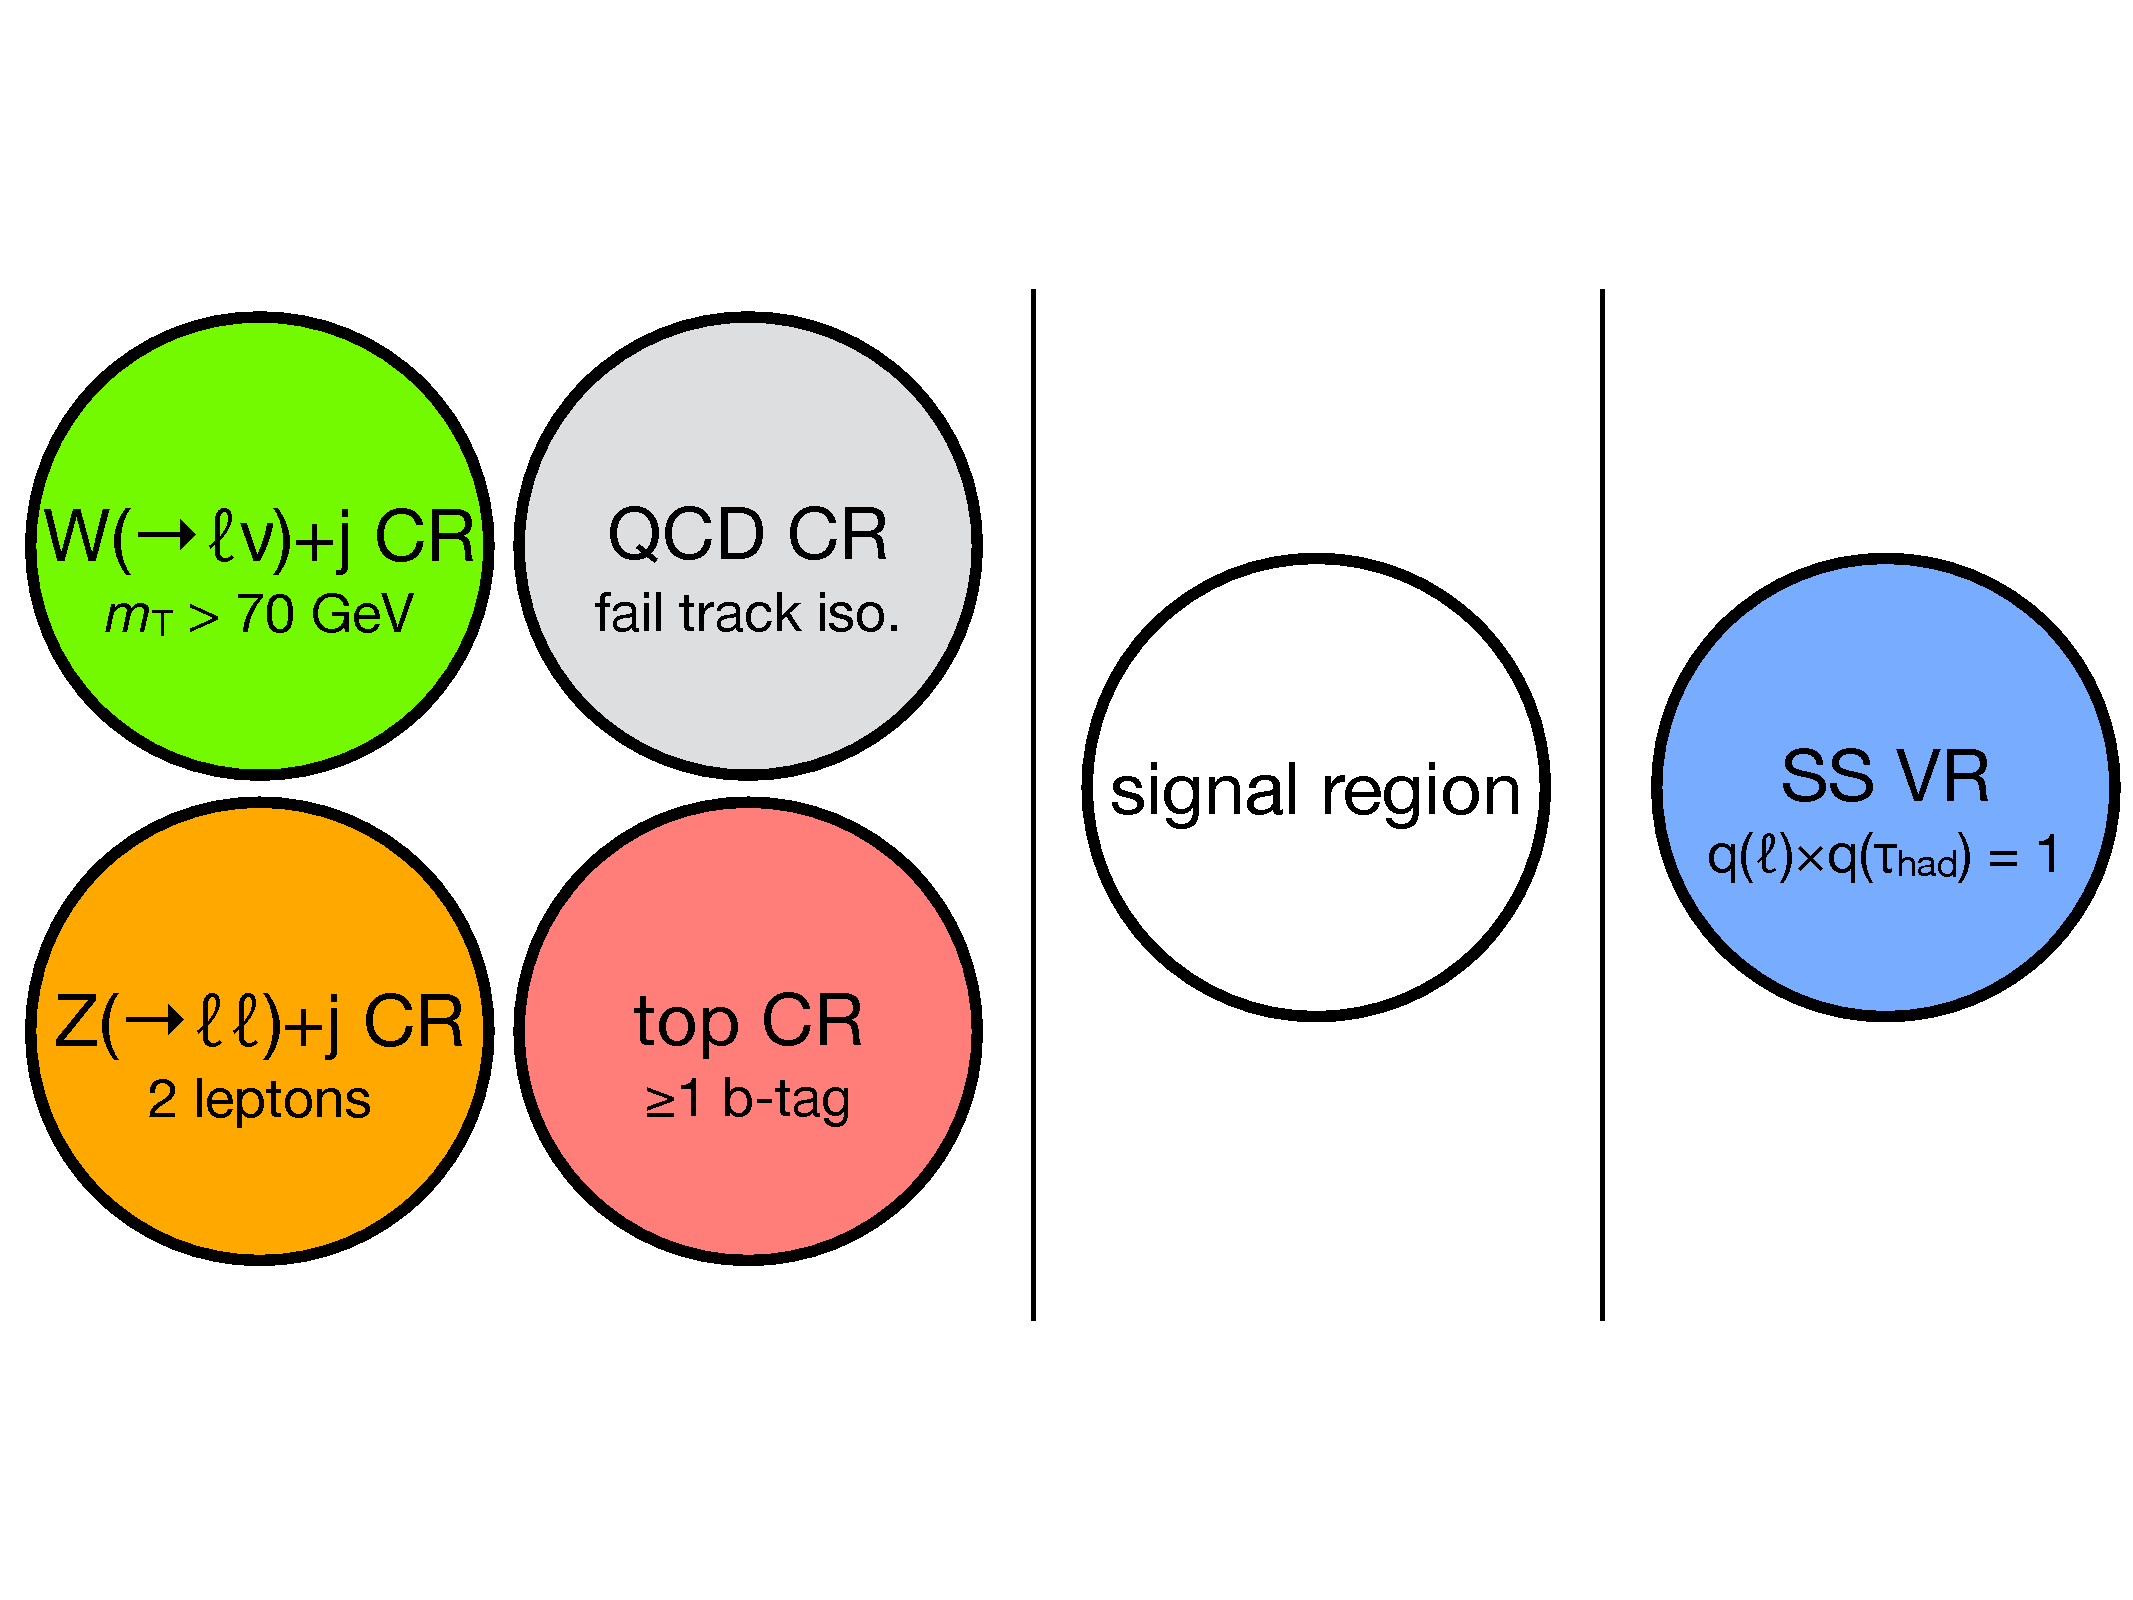
\includegraphics[width=0.90\textwidth]{figures/backgrounds/regions-cartoon}
  \caption{Variables.}
  \label{fig:backgrounds-regions}
\end{figure}

\begin{figure}[tp]
  \centering
  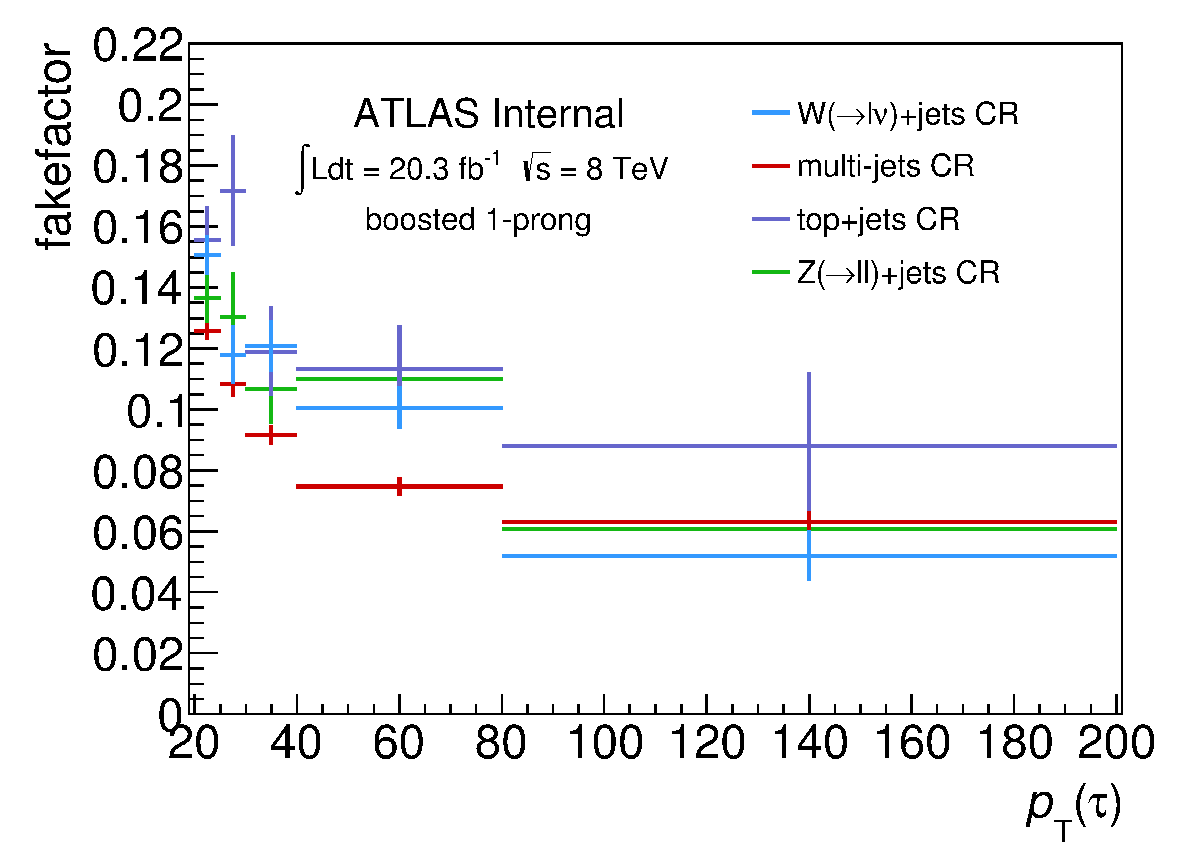
\includegraphics[width=0.48\textwidth]{figures/backgrounds/fakefactor_8TeV_boosted_1p_CRs}
  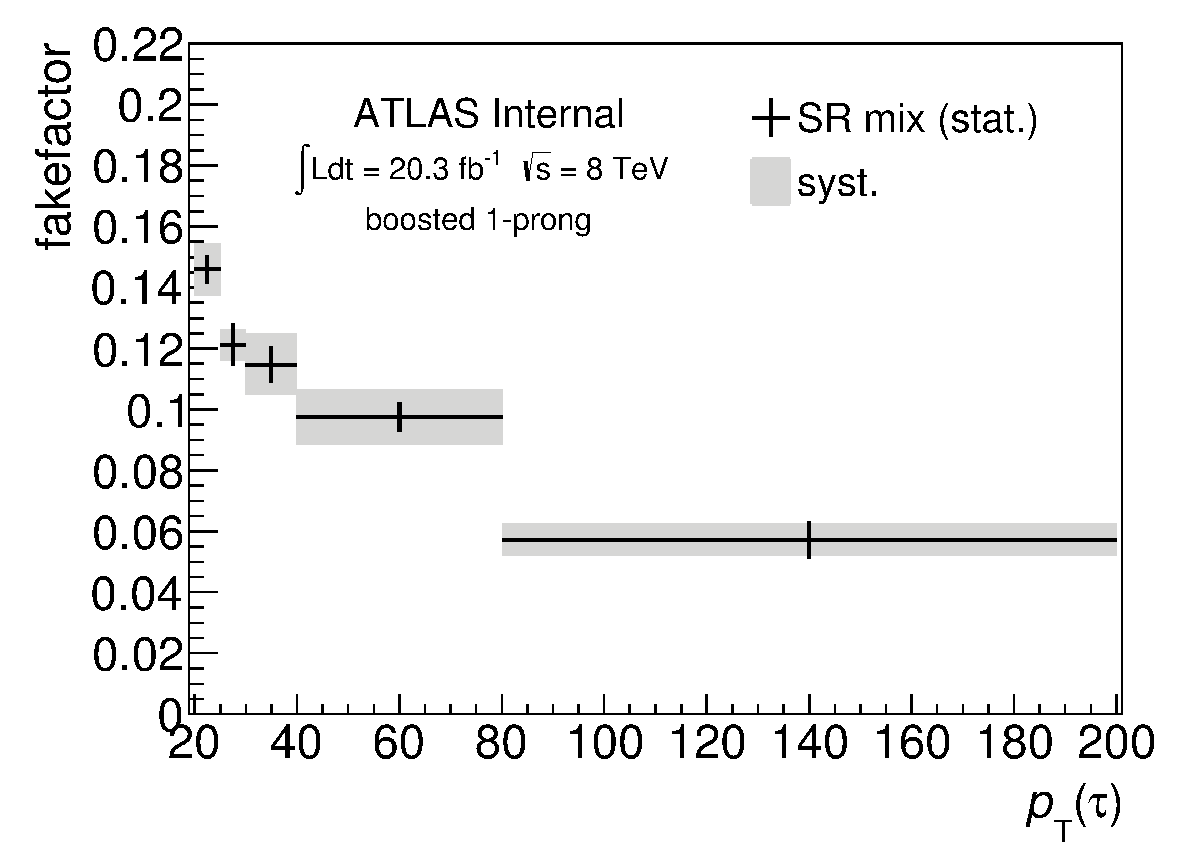
\includegraphics[width=0.48\textwidth]{figures/backgrounds/fakefactor_8TeV_boosted_1p_mix}
  \caption{Variables.}
  \label{fig:backgrounds-fakefactorsboost1p}
\end{figure}

\begin{figure}[tp]
  \centering
  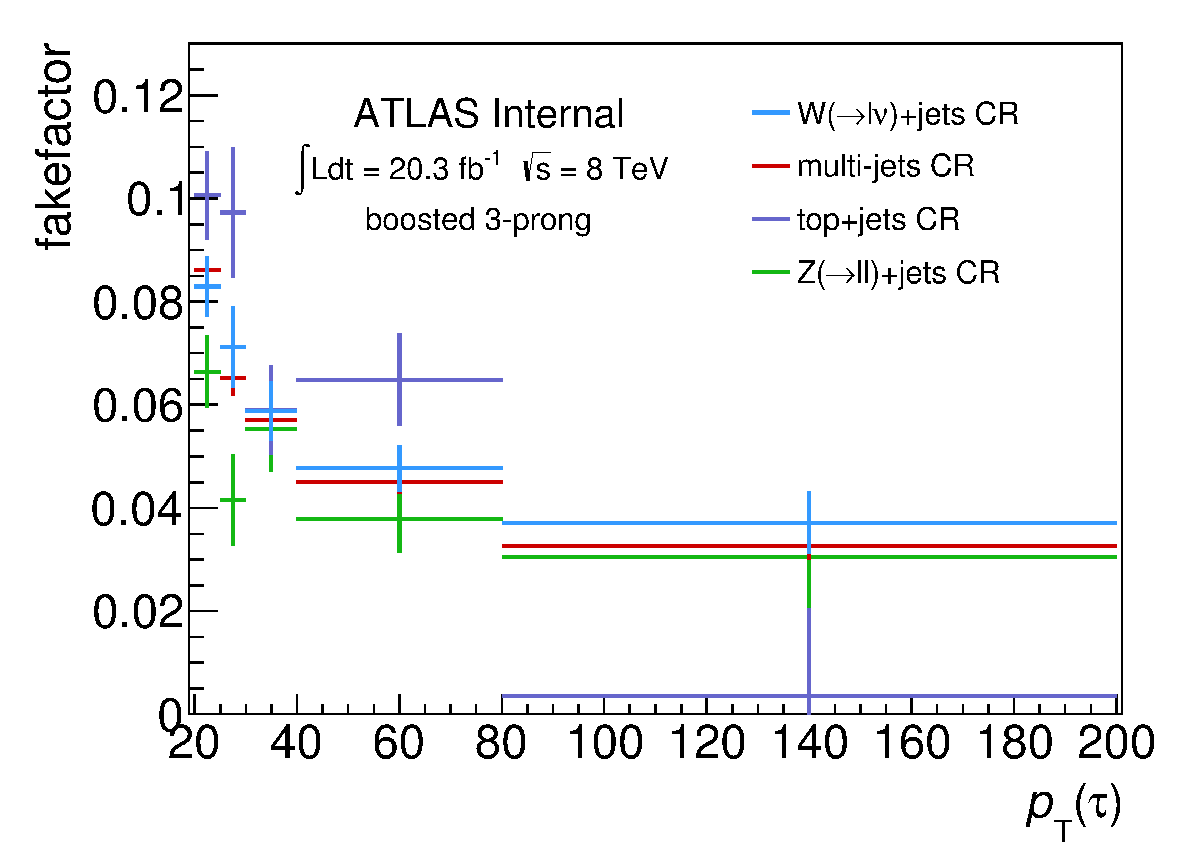
\includegraphics[width=0.48\textwidth]{figures/backgrounds/fakefactor_8TeV_boosted_3p_CRs}
  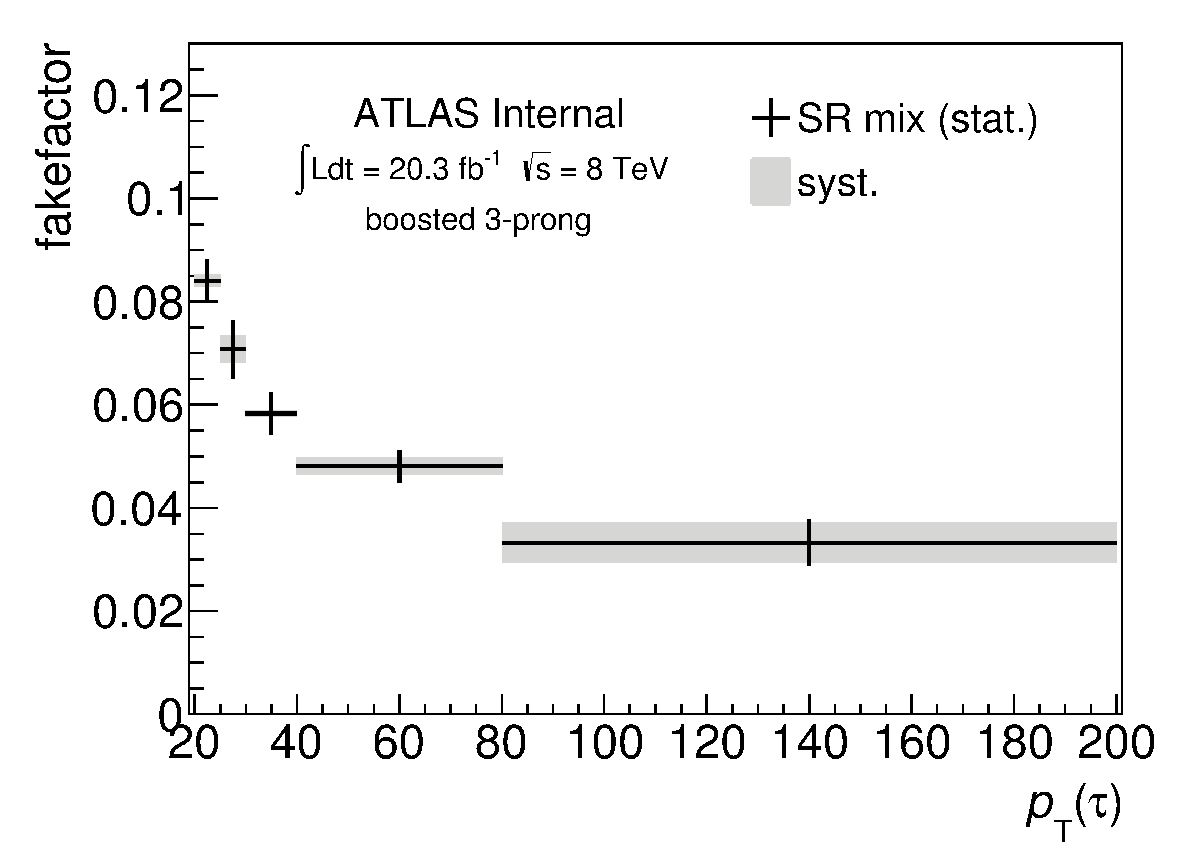
\includegraphics[width=0.48\textwidth]{figures/backgrounds/fakefactor_8TeV_boosted_3p_mix}
  \caption{Variables.}
  \label{fig:backgrounds-fakefactorsboost3p}
\end{figure}

\begin{figure}[tp]
  \centering
  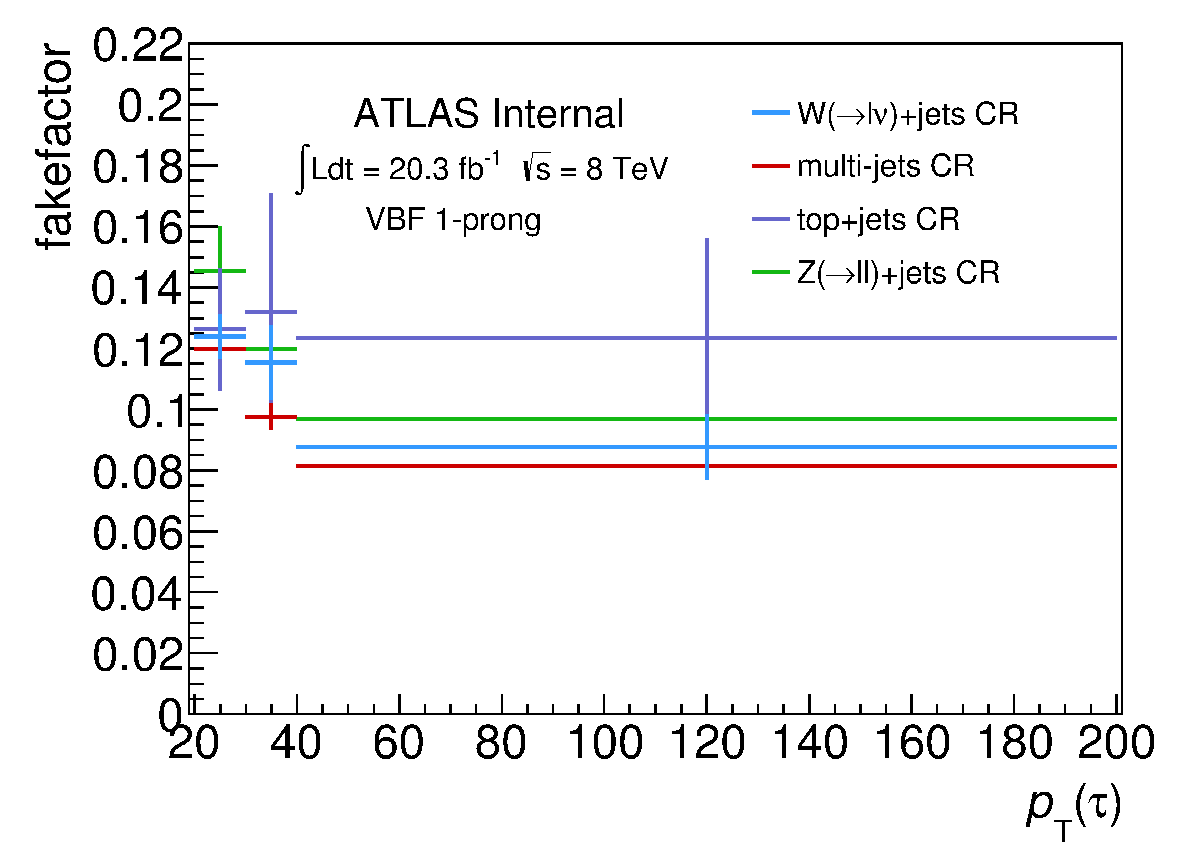
\includegraphics[width=0.48\textwidth]{figures/backgrounds/fakefactor_8TeV_vbf_1p_CRs}
  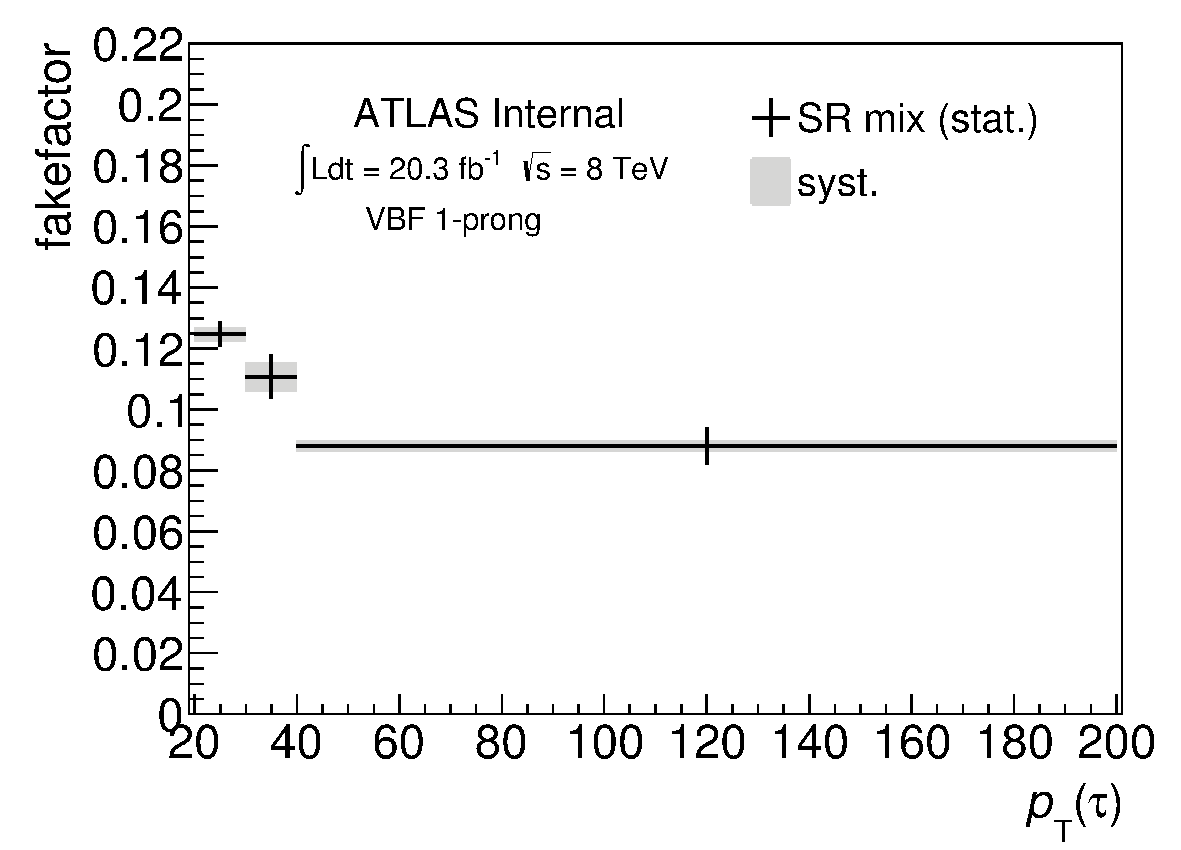
\includegraphics[width=0.48\textwidth]{figures/backgrounds/fakefactor_8TeV_vbf_1p_mix}
  \caption{Variables.}
  \label{fig:backgrounds-fakefactorsVBF1p}
\end{figure}

\begin{figure}[tp]
  \centering
  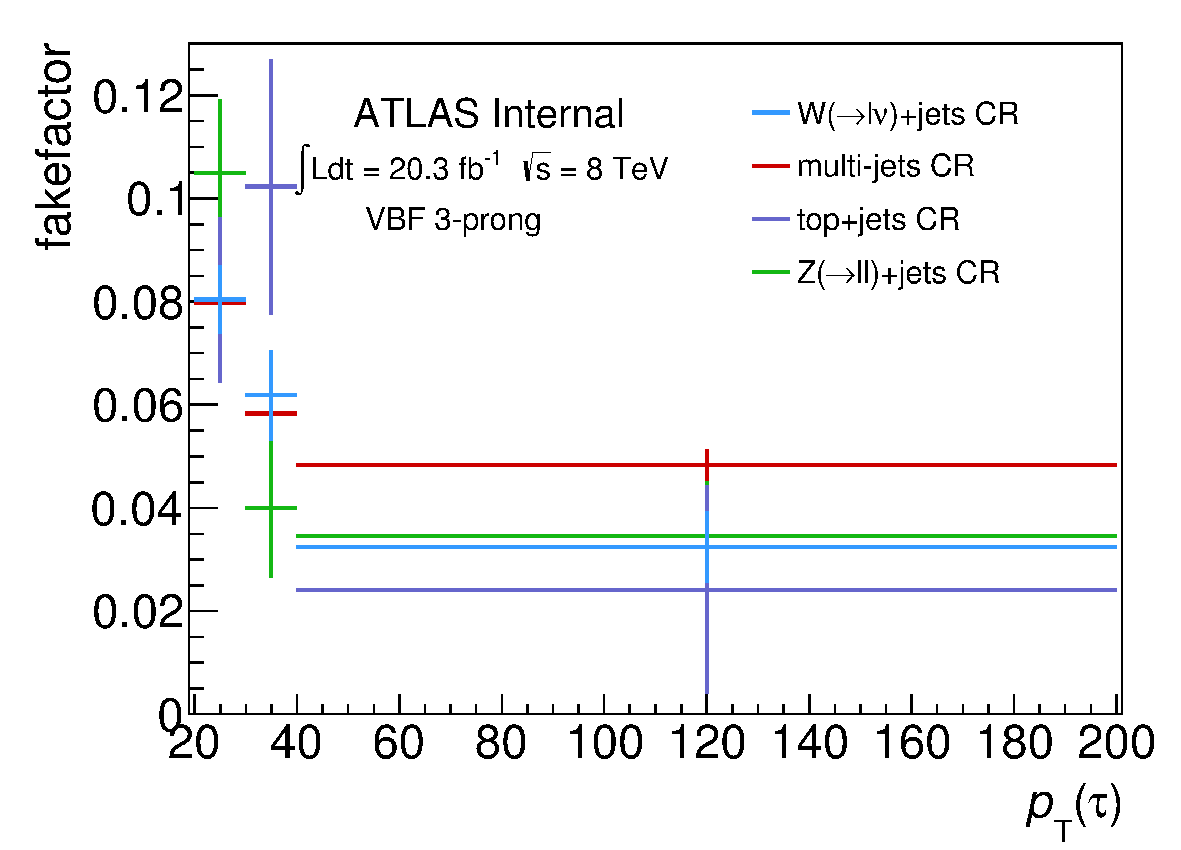
\includegraphics[width=0.48\textwidth]{figures/backgrounds/fakefactor_8TeV_vbf_3p_CRs}
  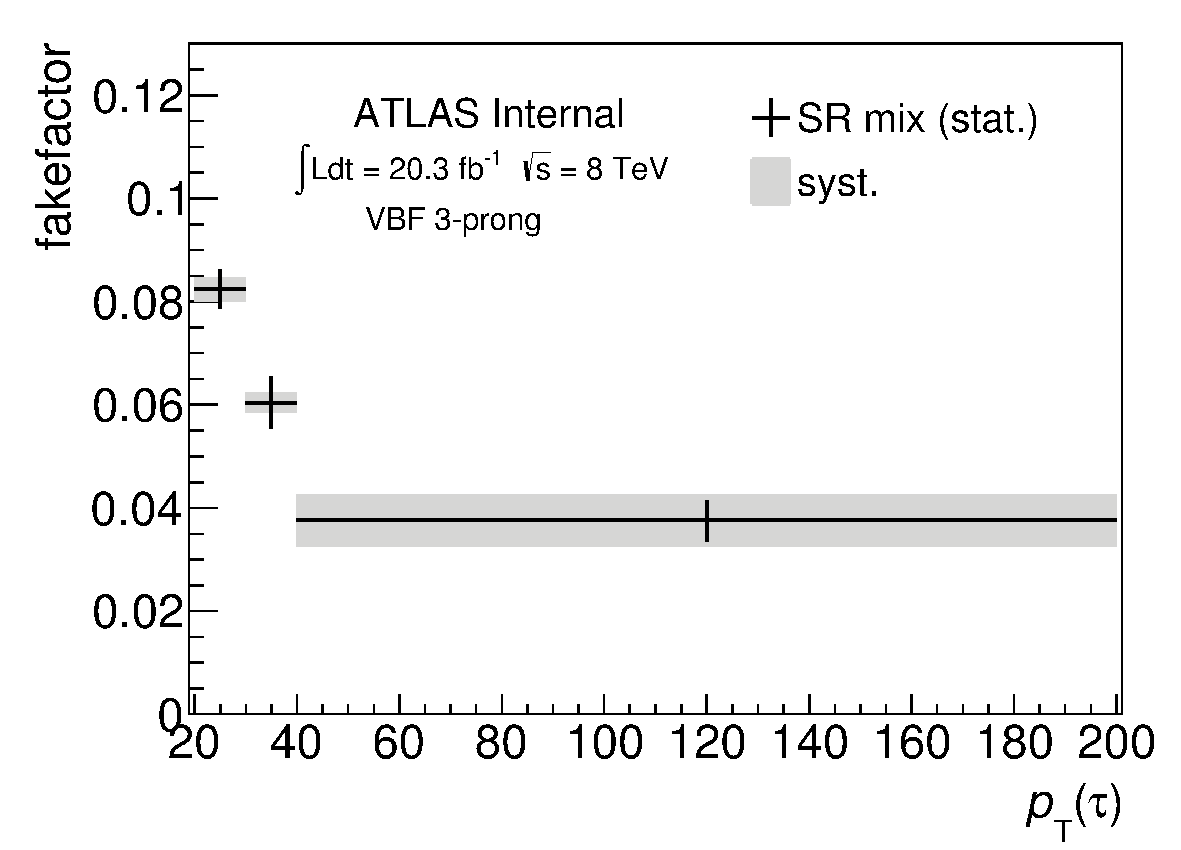
\includegraphics[width=0.48\textwidth]{figures/backgrounds/fakefactor_8TeV_vbf_3p_mix}
  \caption{Variables.}
  \label{fig:backgrounds-fakefactorsVBF3p}
\end{figure}

\clearpage

\begin{figure}[tp]
  \centering
  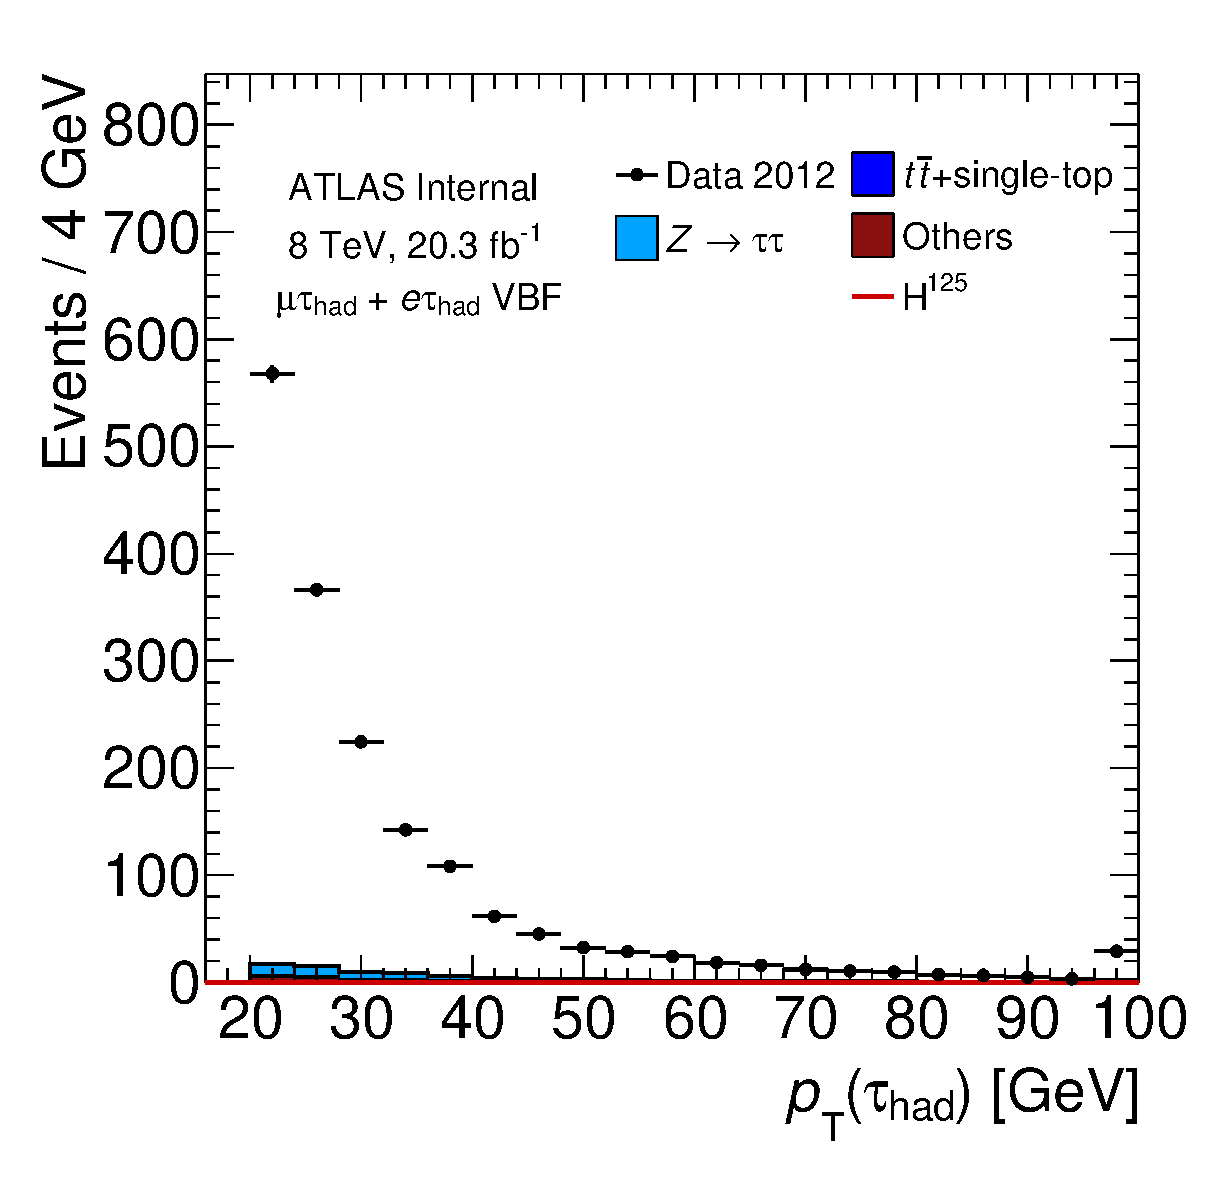
\includegraphics[width=0.32\textwidth]{figures/antitaus/tau-pt}
  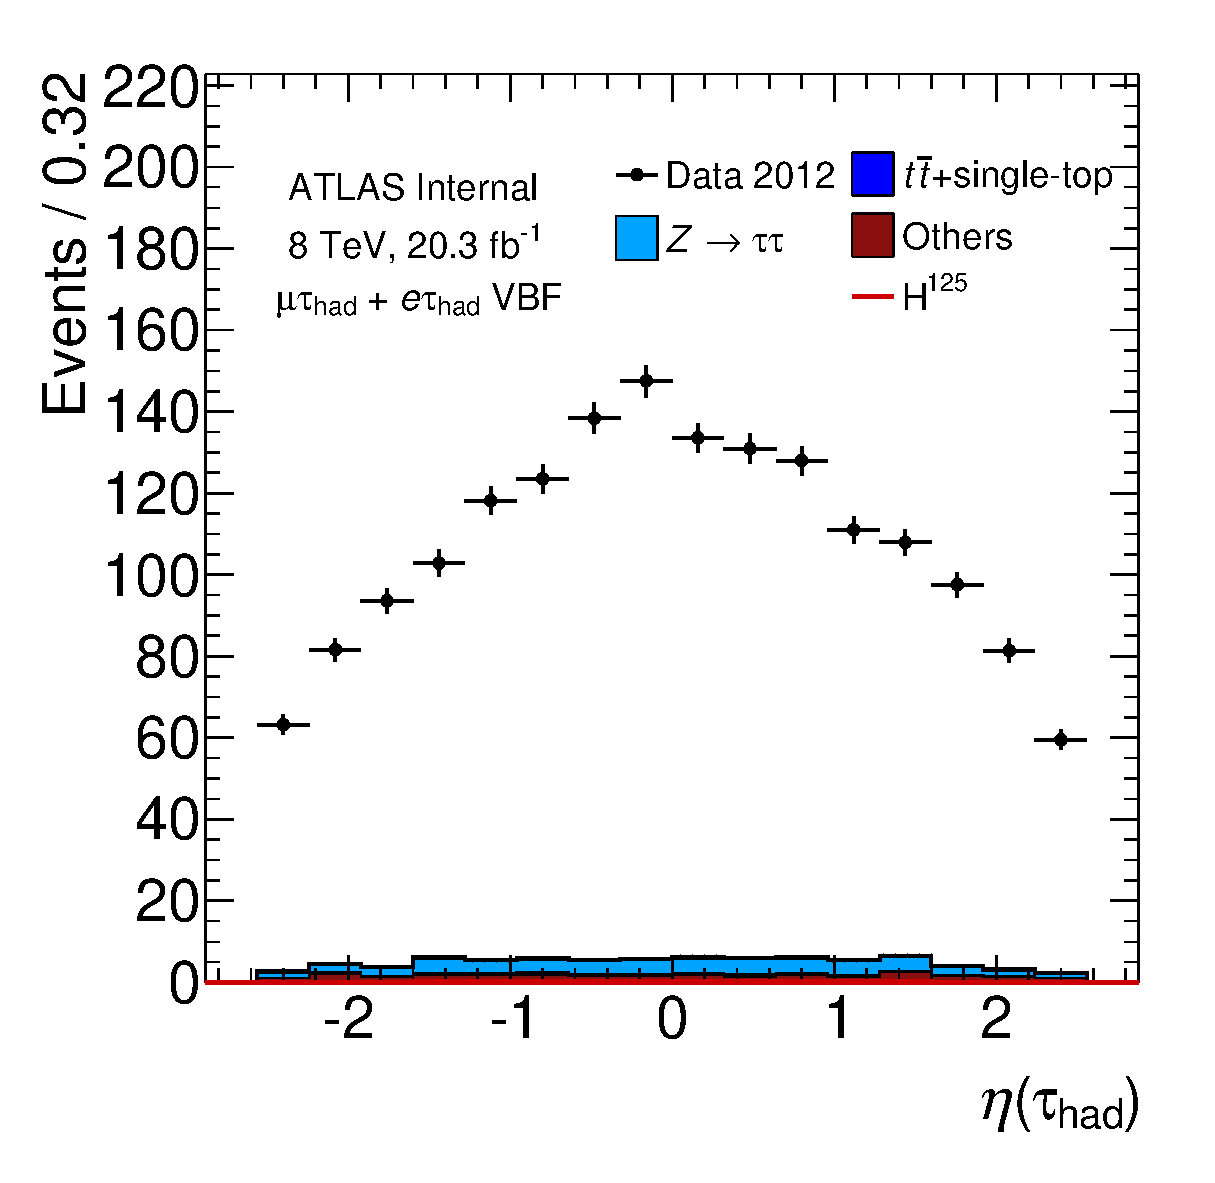
\includegraphics[width=0.32\textwidth]{figures/antitaus/tau-eta}
  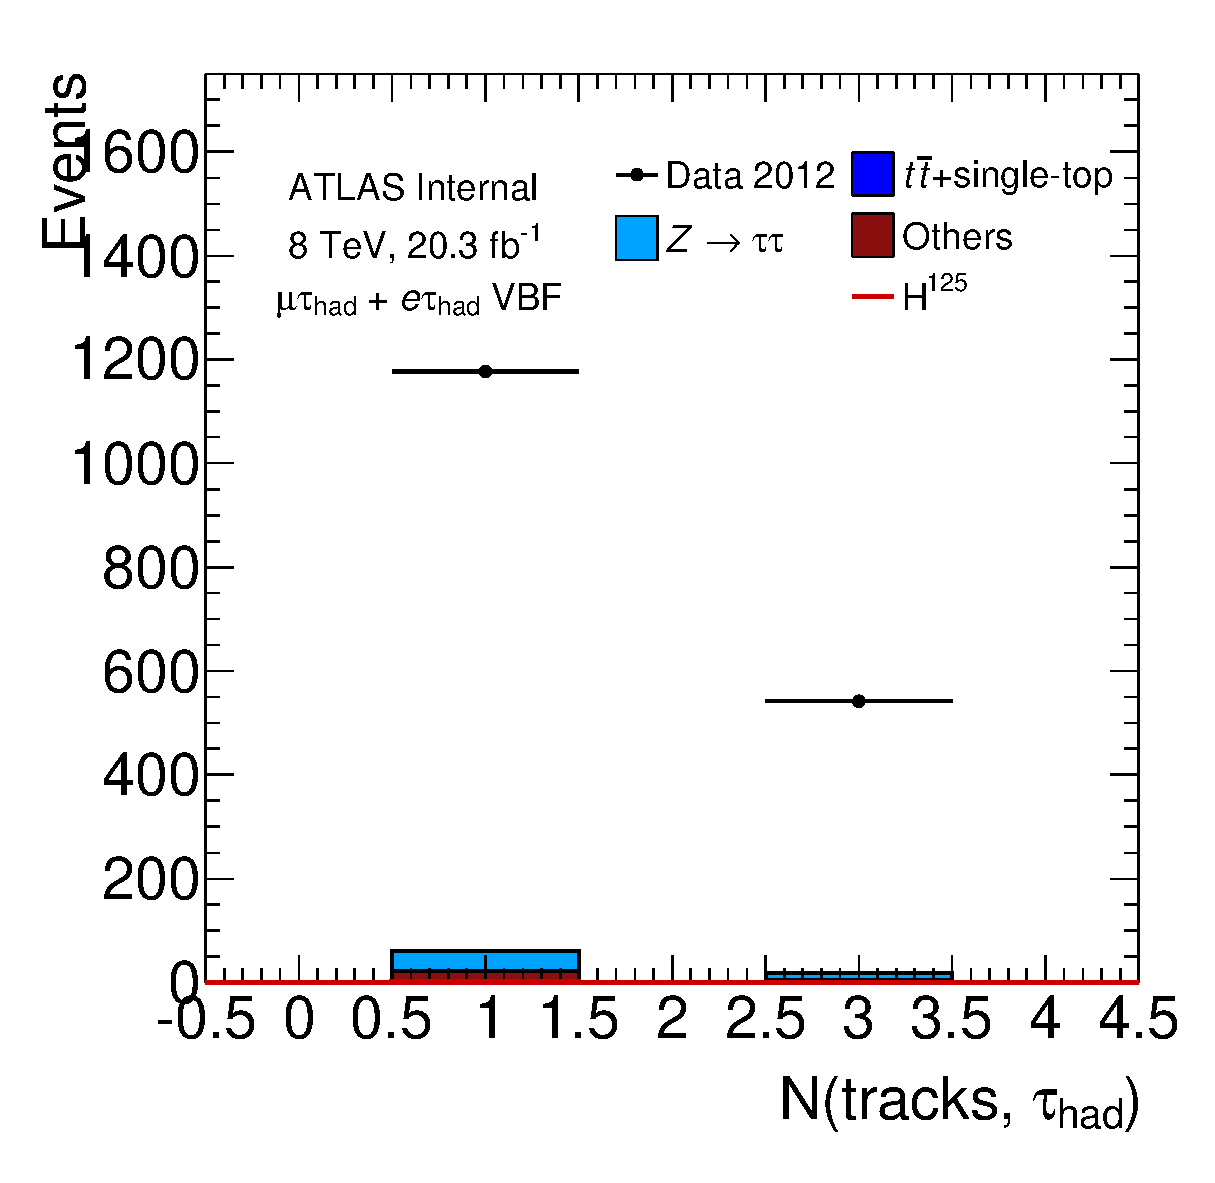
\includegraphics[width=0.32\textwidth]{figures/antitaus/tau-numTrack}
  % --------------
  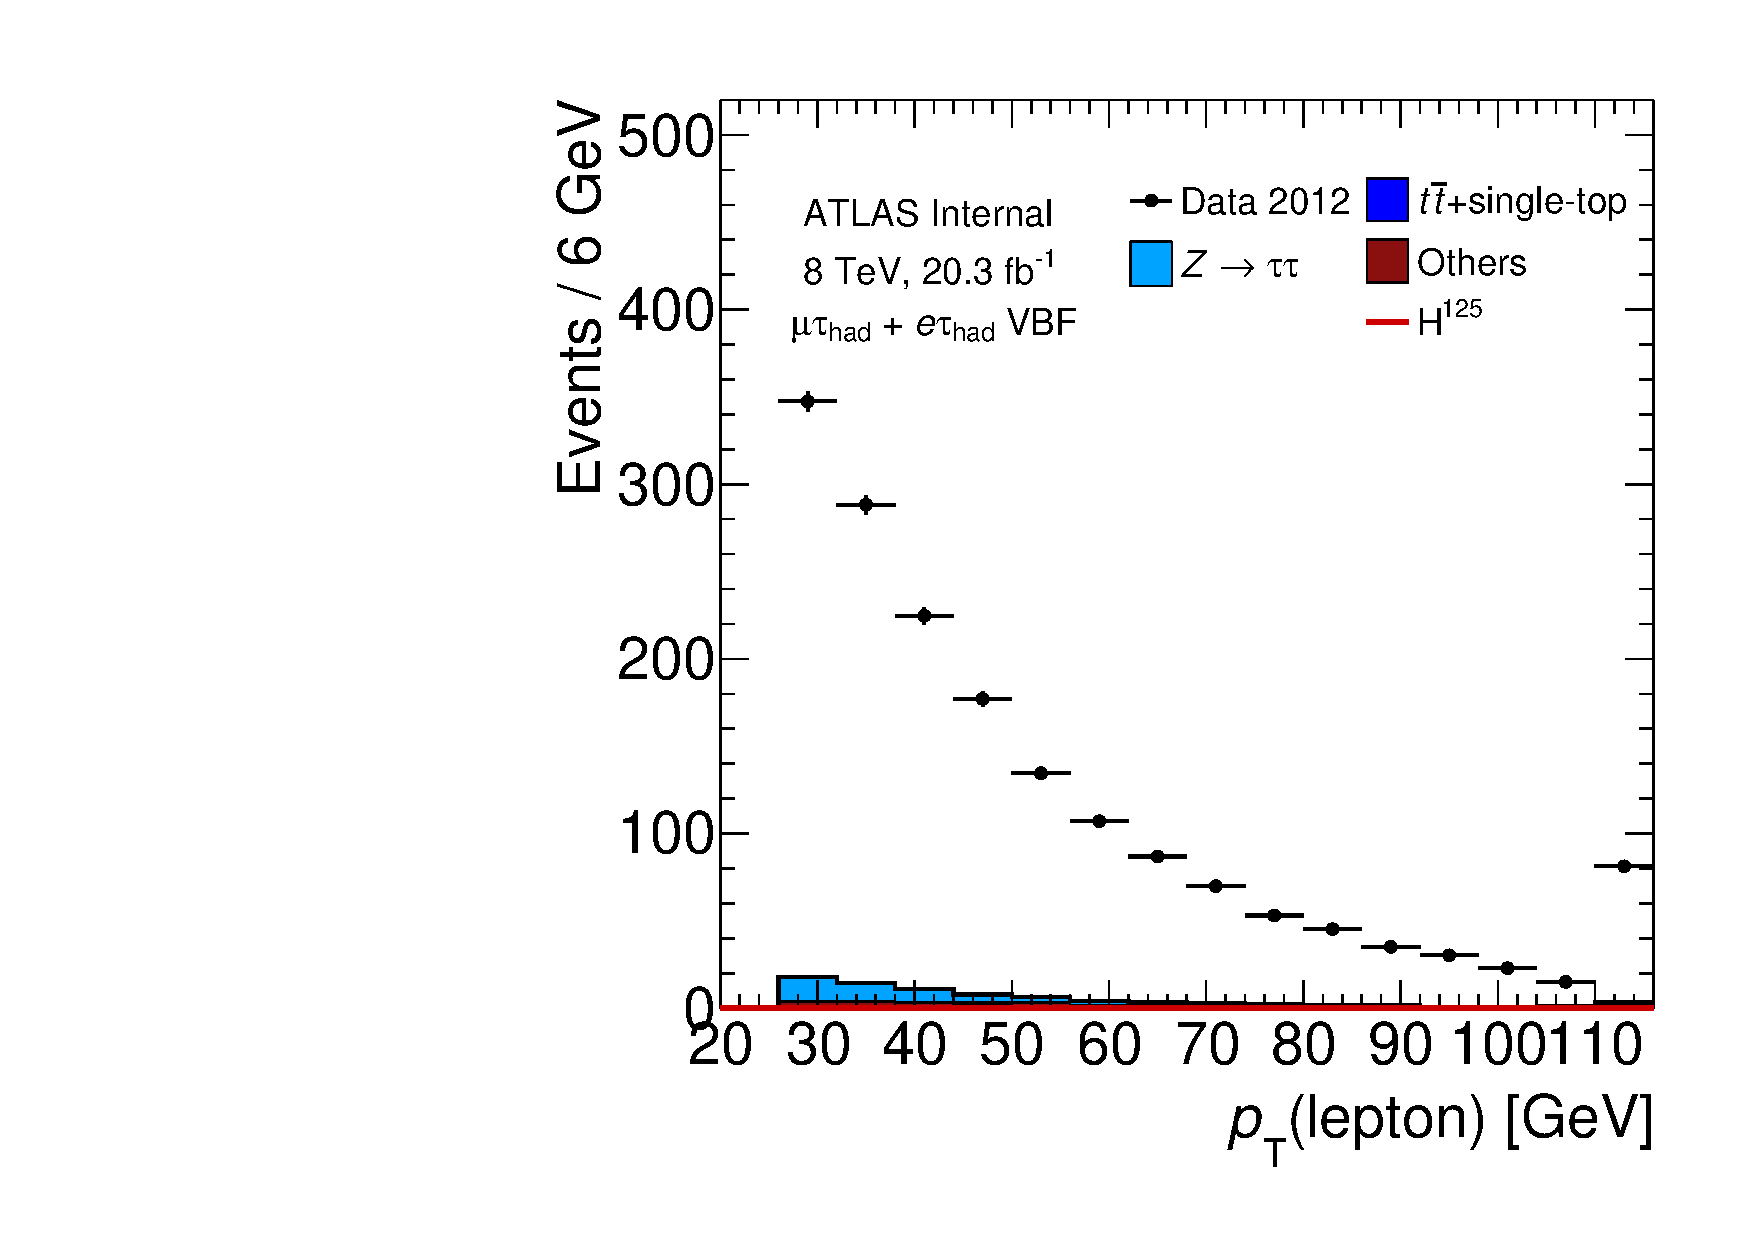
\includegraphics[width=0.32\textwidth]{figures/antitaus/lep-pt-hi}
  \includegraphics[width=0.32\textwidth]{figures/antitaus/lep-eta}
  \includegraphics[width=0.32\textwidth]{figures/antitaus/taulep-dR}
  % --------------
  \includegraphics[width=0.32\textwidth]{figures/antitaus/met-pt-hi}
  \includegraphics[width=0.32\textwidth]{figures/antitaus/mMMC}
  \includegraphics[width=0.32\textwidth]{figures/antitaus/mT}
  % --------------
  \includegraphics[width=0.32\textwidth]{figures/antitaus/met-phi-centrality}
  \includegraphics[width=0.32\textwidth]{figures/antitaus/H-pt-hi}
  \includegraphics[width=0.32\textwidth]{figures/antitaus/mvis}
  \caption{Variables.}
  \label{fig:backgrounds-antitaus-taus}
\end{figure}

\clearpage

\begin{figure}[tp]
  \includegraphics[width=0.32\textwidth]{figures/antitaus/jet-1-pt}
  \includegraphics[width=0.32\textwidth]{figures/antitaus/jet-1-eta}
  \includegraphics[width=0.32\textwidth]{figures/antitaus/jets-dphi}
  % --------------
  \includegraphics[width=0.32\textwidth]{figures/antitaus/jet-2-pt}
  \includegraphics[width=0.32\textwidth]{figures/antitaus/jet-2-eta}
  \includegraphics[width=0.32\textwidth]{figures/antitaus/jets-deta}
  % --------------
  \includegraphics[width=0.32\textwidth]{figures/antitaus/jets-etaprod}
  \includegraphics[width=0.32\textwidth]{figures/antitaus/lep-eta-centrality}
  \includegraphics[width=0.32\textwidth]{figures/antitaus/system-pt}
  % --------------
  \includegraphics[width=0.32\textwidth]{figures/antitaus/n-jets30}
  \includegraphics[width=0.32\textwidth]{figures/antitaus/dijet-m-veryhigh}
  \includegraphics[width=0.32\textwidth]{figures/antitaus/BDTEve-VBF}
  \caption{Variables.}
  \label{fig:backgrounds-antitaus-jets}
\end{figure}

\clearpage

\begin{figure}[tp]
  \includegraphics[width=0.32\textwidth]{figures/tauidcorrelations/tauid_vs_mMMC}
  \includegraphics[width=0.32\textwidth]{figures/tauidcorrelations/tauid_vs_mT}
  \includegraphics[width=0.32\textwidth]{figures/tauidcorrelations/tauid_vs_dR}
  % --------------
  \includegraphics[width=0.32\textwidth]{figures/tauidcorrelations/tauid_vs_metphi}
  \includegraphics[width=0.32\textwidth]{figures/tauidcorrelations/tauid_vs_lepeta}
  \includegraphics[width=0.32\textwidth]{figures/tauidcorrelations/tauid_vs_pttot}
  % --------------
  \includegraphics[width=0.32\textwidth]{figures/tauidcorrelations/tauid_vs_mjj}
  \includegraphics[width=0.32\textwidth]{figures/tauidcorrelations/tauid_vs_detajj}
  \includegraphics[width=0.32\textwidth]{figures/tauidcorrelations/tauid_vs_etaprod}
  % --------------
  \includegraphics[width=0.32\textwidth]{figures/tauidcorrelations/tauid_vs_metet}
  \includegraphics[width=0.32\textwidth]{figures/tauidcorrelations/tauid_vs_Hpt}
  \includegraphics[width=0.32\textwidth]{figures/tauidcorrelations/tauid_vs_bdt}
  \caption{Variables.}
  \label{fig:backgrounds-tauid-correlations}
\end{figure}

\clearpage

\begin{figure}[tp]
  \centering
  \includegraphics[width=0.32\textwidth]{figures/analysis/vbf-SSXCR/tau-pt}
  \includegraphics[width=0.32\textwidth]{figures/analysis/vbf-SSXCR/tau-eta}
  \includegraphics[width=0.32\textwidth]{figures/analysis/vbf-SSXCR/tau-numTrack}
  % --------------
  \includegraphics[width=0.32\textwidth]{figures/analysis/vbf-SSXCR/lep-pt-hi}
  \includegraphics[width=0.32\textwidth]{figures/analysis/vbf-SSXCR/lep-eta}
  \includegraphics[width=0.32\textwidth]{figures/analysis/vbf-SSXCR/taulep-dR}
  % --------------
  \includegraphics[width=0.32\textwidth]{figures/analysis/vbf-SSXCR/met-pt-hi}
  \includegraphics[width=0.32\textwidth]{figures/analysis/vbf-SSXCR/mMMC}
  \includegraphics[width=0.32\textwidth]{figures/analysis/vbf-SSXCR/mT}
  % --------------
  \includegraphics[width=0.32\textwidth]{figures/analysis/vbf-SSXCR/met-phi-centrality}
  \includegraphics[width=0.32\textwidth]{figures/analysis/vbf-SSXCR/H-pt-hi}
  \includegraphics[width=0.32\textwidth]{figures/analysis/vbf-SSXCR/mvis}
  \caption{Variables.}
  \label{fig:backgrounds-SSXCR-taus}
\end{figure}

\clearpage
\begin{figure}[tp]
  \includegraphics[width=0.32\textwidth]{figures/analysis/vbf-SSXCR/jet-1-pt}
  \includegraphics[width=0.32\textwidth]{figures/analysis/vbf-SSXCR/jet-1-eta}
  \includegraphics[width=0.32\textwidth]{figures/analysis/vbf-SSXCR/jets-dphi}
  % --------------
  \includegraphics[width=0.32\textwidth]{figures/analysis/vbf-SSXCR/jet-2-pt}
  \includegraphics[width=0.32\textwidth]{figures/analysis/vbf-SSXCR/jet-2-eta}
  \includegraphics[width=0.32\textwidth]{figures/analysis/vbf-SSXCR/jets-deta}
  % --------------
  \includegraphics[width=0.32\textwidth]{figures/analysis/vbf-SSXCR/jets-etaprod}
  \includegraphics[width=0.32\textwidth]{figures/analysis/vbf-SSXCR/lep-eta-centrality}
  \includegraphics[width=0.32\textwidth]{figures/analysis/vbf-SSXCR/system-pt}
  % --------------
  \includegraphics[width=0.32\textwidth]{figures/analysis/vbf-SSXCR/n-jets30}
  \includegraphics[width=0.32\textwidth]{figures/analysis/vbf-SSXCR/dijet-m-veryhigh}
  \includegraphics[width=0.32\textwidth]{figures/analysis/vbf-SSXCR/BDTEve-VBF}
  \caption{Variables.}
  \label{fig:backgrounds-SSXCR-jets}
\end{figure}

\clearpage
\begin{figure}[tp]
  \centering
  \includegraphics[width=0.32\textwidth]{figures/analysis/vbf-MCXSR/tau-pt}
  \includegraphics[width=0.32\textwidth]{figures/analysis/vbf-MCXSR/tau-eta}
  \includegraphics[width=0.32\textwidth]{figures/analysis/vbf-MCXSR/tau-numTrack}
  % --------------
  \includegraphics[width=0.32\textwidth]{figures/analysis/vbf-MCXSR/lep-pt-hi}
  \includegraphics[width=0.32\textwidth]{figures/analysis/vbf-MCXSR/lep-eta}
  \includegraphics[width=0.32\textwidth]{figures/analysis/vbf-MCXSR/taulep-dR}
  % --------------
  \includegraphics[width=0.32\textwidth]{figures/analysis/vbf-MCXSR/met-pt-hi}
  \includegraphics[width=0.32\textwidth]{figures/analysis/vbf-MCXSR/mMMC}
  \includegraphics[width=0.32\textwidth]{figures/analysis/vbf-MCXSR/mT}
  % --------------
  \includegraphics[width=0.32\textwidth]{figures/analysis/vbf-MCXSR/met-phi-centrality}
  \includegraphics[width=0.32\textwidth]{figures/analysis/vbf-MCXSR/H-pt-hi}
  \includegraphics[width=0.32\textwidth]{figures/analysis/vbf-MCXSR/mvis}
  \caption{Variables.}
  \label{fig:backgrounds-MCXSR-taus}
\end{figure}

\clearpage
\begin{figure}[tp]
  \includegraphics[width=0.32\textwidth]{figures/analysis/vbf-MCXSR/jet-1-pt}
  \includegraphics[width=0.32\textwidth]{figures/analysis/vbf-MCXSR/jet-1-eta}
  \includegraphics[width=0.32\textwidth]{figures/analysis/vbf-MCXSR/jets-dphi}
  % --------------
  \includegraphics[width=0.32\textwidth]{figures/analysis/vbf-MCXSR/jet-2-pt}
  \includegraphics[width=0.32\textwidth]{figures/analysis/vbf-MCXSR/jet-2-eta}
  \includegraphics[width=0.32\textwidth]{figures/analysis/vbf-MCXSR/jets-deta}
  % --------------
  \includegraphics[width=0.32\textwidth]{figures/analysis/vbf-MCXSR/jets-etaprod}
  \includegraphics[width=0.32\textwidth]{figures/analysis/vbf-MCXSR/lep-eta-centrality}
  \includegraphics[width=0.32\textwidth]{figures/analysis/vbf-MCXSR/system-pt}
  % --------------
  \includegraphics[width=0.32\textwidth]{figures/analysis/vbf-MCXSR/n-jets30}
  \includegraphics[width=0.32\textwidth]{figures/analysis/vbf-MCXSR/dijet-m-high}
  \includegraphics[width=0.32\textwidth]{figures/analysis/vbf-MCXSR/BDTEve-VBF}
  \caption{Variables.}
  \label{fig:backgrounds-MCXSR-jets}
\end{figure}

\clearpage
\begin{figure}[tp]
  \includegraphics[width=0.90\textwidth]{figures/uncertainties/uncertainties_lephad_paper14_8TeV_fakes_VBF}
  \caption{Variables.}
  \label{fig:backgrounds-uncertainties-fakes}
\end{figure}

\clearpage
\section{$\Htautau$, VBF}
\label{sec:backgrounds-vbfhtautau}

\begin{figure}[tp]
  \includegraphics[width=0.90\textwidth]{figures/uncertainties/uncertainties_lephad_paper14_8TeV_VBFH125_JES_VBF}
  \caption{Variables.}
  \label{fig:backgrounds-uncertainties-vbfjes}
\end{figure}

\begin{figure}[tp]
  \includegraphics[width=0.90\textwidth]{figures/uncertainties/uncertainties_lephad_paper14_8TeV_VBFH125_other_VBF}
  \caption{Variables.}
  \label{fig:backgrounds-uncertainties-vbfother}
\end{figure}

\section{$\Htautau$, ggF}
\label{sec:backgrounds-ggfhtautau}

